% Options for packages loaded elsewhere
\PassOptionsToPackage{unicode}{hyperref}
\PassOptionsToPackage{hyphens}{url}
\PassOptionsToPackage{dvipsnames,svgnames,x11names}{xcolor}
%
\documentclass[
  12pt,
  a4paper,
  extrafontsizes,
  onecolumn,
  openright,
  table]{memoir}

\usepackage{amsmath,amssymb}
\usepackage{iftex}
\ifPDFTeX
  \usepackage[T1]{fontenc}
  \usepackage[utf8]{inputenc}
  \usepackage{textcomp} % provide euro and other symbols
\else % if luatex or xetex
  \usepackage{unicode-math}
  \defaultfontfeatures{Scale=MatchLowercase}
  \defaultfontfeatures[\rmfamily]{Ligatures=TeX,Scale=1}
\fi
\usepackage{lmodern}
\ifPDFTeX\else  
    % xetex/luatex font selection
  \setmainfont[Extension=.otf,UprightFont=*-regular,BoldFont=*-bold,BoldItalicFont=*-bolditalic,ItalicFont=*-italic]{texgyretermes}
  \setmathfont[]{texgyretermes-math.otf}
\fi
% Use upquote if available, for straight quotes in verbatim environments
\IfFileExists{upquote.sty}{\usepackage{upquote}}{}
\IfFileExists{microtype.sty}{% use microtype if available
  \usepackage[]{microtype}
  \UseMicrotypeSet[protrusion]{basicmath} % disable protrusion for tt fonts
}{}
\makeatletter
\@ifundefined{KOMAClassName}{% if non-KOMA class
  \IfFileExists{parskip.sty}{%
    \usepackage{parskip}
  }{% else
    \setlength{\parindent}{0pt}
    \setlength{\parskip}{6pt plus 2pt minus 1pt}}
}{% if KOMA class
  \KOMAoptions{parskip=half}}
\makeatother
\usepackage{xcolor}
\setlength{\emergencystretch}{3em} % prevent overfull lines
\setcounter{secnumdepth}{5}
% Make \paragraph and \subparagraph free-standing
\ifx\paragraph\undefined\else
  \let\oldparagraph\paragraph
  \renewcommand{\paragraph}[1]{\oldparagraph{#1}\mbox{}}
\fi
\ifx\subparagraph\undefined\else
  \let\oldsubparagraph\subparagraph
  \renewcommand{\subparagraph}[1]{\oldsubparagraph{#1}\mbox{}}
\fi
% pandoc tempate
%%%%%%%%%%%%%%%%%%%%%%%%%%%%%%%%%%%%%%%%%%%%%%%%%%%%%%%%%%

\usepackage{color}
\usepackage{fancyvrb}
\newcommand{\VerbBar}{|}
\newcommand{\VERB}{\Verb[commandchars=\\\{\}]}
\DefineVerbatimEnvironment{Highlighting}{Verbatim}{commandchars=\\\{\}}
% Add ',fontsize=\small' for more characters per line
\usepackage{framed}
\definecolor{shadecolor}{RGB}{241,243,245}
\newenvironment{Shaded}{\begin{snugshade}}{\end{snugshade}}
\newcommand{\AlertTok}[1]{\textcolor[rgb]{0.68,0.00,0.00}{#1}}
\newcommand{\AnnotationTok}[1]{\textcolor[rgb]{0.37,0.37,0.37}{#1}}
\newcommand{\AttributeTok}[1]{\textcolor[rgb]{0.40,0.45,0.13}{#1}}
\newcommand{\BaseNTok}[1]{\textcolor[rgb]{0.68,0.00,0.00}{#1}}
\newcommand{\BuiltInTok}[1]{\textcolor[rgb]{0.00,0.23,0.31}{#1}}
\newcommand{\CharTok}[1]{\textcolor[rgb]{0.13,0.47,0.30}{#1}}
\newcommand{\CommentTok}[1]{\textcolor[rgb]{0.37,0.37,0.37}{#1}}
\newcommand{\CommentVarTok}[1]{\textcolor[rgb]{0.37,0.37,0.37}{\textit{#1}}}
\newcommand{\ConstantTok}[1]{\textcolor[rgb]{0.56,0.35,0.01}{#1}}
\newcommand{\ControlFlowTok}[1]{\textcolor[rgb]{0.00,0.23,0.31}{#1}}
\newcommand{\DataTypeTok}[1]{\textcolor[rgb]{0.68,0.00,0.00}{#1}}
\newcommand{\DecValTok}[1]{\textcolor[rgb]{0.68,0.00,0.00}{#1}}
\newcommand{\DocumentationTok}[1]{\textcolor[rgb]{0.37,0.37,0.37}{\textit{#1}}}
\newcommand{\ErrorTok}[1]{\textcolor[rgb]{0.68,0.00,0.00}{#1}}
\newcommand{\ExtensionTok}[1]{\textcolor[rgb]{0.00,0.23,0.31}{#1}}
\newcommand{\FloatTok}[1]{\textcolor[rgb]{0.68,0.00,0.00}{#1}}
\newcommand{\FunctionTok}[1]{\textcolor[rgb]{0.28,0.35,0.67}{#1}}
\newcommand{\ImportTok}[1]{\textcolor[rgb]{0.00,0.46,0.62}{#1}}
\newcommand{\InformationTok}[1]{\textcolor[rgb]{0.37,0.37,0.37}{#1}}
\newcommand{\KeywordTok}[1]{\textcolor[rgb]{0.00,0.23,0.31}{#1}}
\newcommand{\NormalTok}[1]{\textcolor[rgb]{0.00,0.23,0.31}{#1}}
\newcommand{\OperatorTok}[1]{\textcolor[rgb]{0.37,0.37,0.37}{#1}}
\newcommand{\OtherTok}[1]{\textcolor[rgb]{0.00,0.23,0.31}{#1}}
\newcommand{\PreprocessorTok}[1]{\textcolor[rgb]{0.68,0.00,0.00}{#1}}
\newcommand{\RegionMarkerTok}[1]{\textcolor[rgb]{0.00,0.23,0.31}{#1}}
\newcommand{\SpecialCharTok}[1]{\textcolor[rgb]{0.37,0.37,0.37}{#1}}
\newcommand{\SpecialStringTok}[1]{\textcolor[rgb]{0.13,0.47,0.30}{#1}}
\newcommand{\StringTok}[1]{\textcolor[rgb]{0.13,0.47,0.30}{#1}}
\newcommand{\VariableTok}[1]{\textcolor[rgb]{0.07,0.07,0.07}{#1}}
\newcommand{\VerbatimStringTok}[1]{\textcolor[rgb]{0.13,0.47,0.30}{#1}}
\newcommand{\WarningTok}[1]{\textcolor[rgb]{0.37,0.37,0.37}{\textit{#1}}}

\providecommand{\tightlist}{%
  \setlength{\itemsep}{0pt}\setlength{\parskip}{0pt}}\usepackage{longtable,booktabs,array}
\usepackage{calc} % for calculating minipage widths
% Correct order of tables after \paragraph or \subparagraph
\usepackage{etoolbox}
\makeatletter
\patchcmd\longtable{\par}{\if@noskipsec\mbox{}\fi\par}{}{}
\makeatother
% Allow footnotes in longtable head/foot
\IfFileExists{footnotehyper.sty}{\usepackage{footnotehyper}}{\usepackage{footnote}}
\makesavenoteenv{longtable}
\usepackage{graphicx}
\makeatletter
\def\maxwidth{\ifdim\Gin@nat@width>\linewidth\linewidth\else\Gin@nat@width\fi}
\def\maxheight{\ifdim\Gin@nat@height>\textheight\textheight\else\Gin@nat@height\fi}
\makeatother
% Scale images if necessary, so that they will not overflow the page
% margins by default, and it is still possible to overwrite the defaults
% using explicit options in \includegraphics[width, height, ...]{}
\setkeys{Gin}{width=\maxwidth,height=\maxheight,keepaspectratio}
% Set default figure placement to htbp
\makeatletter
\def\fps@figure{htbp}
\makeatother

% Add LaTeX code into the preamble of the document here
\hyphenation{bio-di-ver-si-ty sap-lings}

% Define colors for text boxes
\definecolor{grey}{HTML}{F5F5F5}

% Define text box environments
\usepackage[tikz]{bclogo}
\newmdenv[
  style=boxstyle,
  backgroundcolor=grey,
  frametitlebackgroundcolor=grey,
]{greybox}

\usepackage[automake]{glossaries-extra}
\makeglossaries
\glsenablehyper

\usepackage{multirow}
\usepackage{booktabs}

\usepackage{booktabs}
\usepackage{longtable}
\usepackage{array}
\usepackage{multirow}
\usepackage{wrapfig}
\usepackage{float}
\usepackage{colortbl}
\usepackage{pdflscape}
\usepackage{tabu}
\usepackage{threeparttable}
\usepackage{threeparttablex}
\usepackage[normalem]{ulem}
\usepackage{makecell}
\usepackage{xcolor}
\usepackage{caption}
\usepackage{siunitx}

  \newcolumntype{d}{S[
    input-open-uncertainty=,
    input-close-uncertainty=,
    parse-numbers = false,
    table-align-text-pre=false,
    table-align-text-post=false
  ]}
  
\makeatletter
\@ifpackageloaded{tcolorbox}{}{\usepackage[skins,breakable]{tcolorbox}}
\@ifpackageloaded{fontawesome5}{}{\usepackage{fontawesome5}}
\definecolor{quarto-callout-color}{HTML}{909090}
\definecolor{quarto-callout-note-color}{HTML}{0758E5}
\definecolor{quarto-callout-important-color}{HTML}{CC1914}
\definecolor{quarto-callout-warning-color}{HTML}{EB9113}
\definecolor{quarto-callout-tip-color}{HTML}{00A047}
\definecolor{quarto-callout-caution-color}{HTML}{FC5300}
\definecolor{quarto-callout-color-frame}{HTML}{acacac}
\definecolor{quarto-callout-note-color-frame}{HTML}{4582ec}
\definecolor{quarto-callout-important-color-frame}{HTML}{d9534f}
\definecolor{quarto-callout-warning-color-frame}{HTML}{f0ad4e}
\definecolor{quarto-callout-tip-color-frame}{HTML}{02b875}
\definecolor{quarto-callout-caution-color-frame}{HTML}{fd7e14}
\makeatother
\makeatletter
\makeatother
\makeatletter
\@ifpackageloaded{bookmark}{}{\usepackage{bookmark}}
\makeatother
\makeatletter
\@ifpackageloaded{caption}{}{\usepackage{caption}}
\AtBeginDocument{%
\ifdefined\contentsname
  \renewcommand*\contentsname{Tabla de contenidos}
\else
  \newcommand\contentsname{Tabla de contenidos}
\fi
\ifdefined\listfigurename
  \renewcommand*\listfigurename{Listado de Figuras}
\else
  \newcommand\listfigurename{Listado de Figuras}
\fi
\ifdefined\listtablename
  \renewcommand*\listtablename{Listado de Tablas}
\else
  \newcommand\listtablename{Listado de Tablas}
\fi
\ifdefined\figurename
  \renewcommand*\figurename{Figura}
\else
  \newcommand\figurename{Figura}
\fi
\ifdefined\tablename
  \renewcommand*\tablename{Tabla}
\else
  \newcommand\tablename{Tabla}
\fi
}
\@ifpackageloaded{float}{}{\usepackage{float}}
\floatstyle{ruled}
\@ifundefined{c@chapter}{\newfloat{codelisting}{h}{lop}}{\newfloat{codelisting}{h}{lop}[chapter]}
\floatname{codelisting}{Listado}
\newcommand*\listoflistings{\listof{codelisting}{Listado de Listados}}
\makeatother
\makeatletter
\@ifpackageloaded{caption}{}{\usepackage{caption}}
\@ifpackageloaded{subcaption}{}{\usepackage{subcaption}}
\makeatother
\makeatletter
\@ifpackageloaded{tcolorbox}{}{\usepackage[skins,breakable]{tcolorbox}}
\makeatother
\makeatletter
\@ifundefined{shadecolor}{\definecolor{shadecolor}{rgb}{.97, .97, .97}}
\makeatother
\makeatletter
\makeatother
\makeatletter
\makeatother


% Additional content
%%%%%%%%%%%%%%%%%%%%%%%%%%%%%%%%%%%%%%%%%%%%%%%%%%%%%%%%%%

\graphicspath{{images/}}


% Chapter Summary environment
%%%%%%%%%%%%%%%%%%%%%%%%%%%%%%%
\usepackage[tikz]{bclogo}
\newenvironment{Summary}
  {\begin{bclogo}[logo=\bctrombone, noborder=true, couleur=lightgray!50]{En
resumen}\parindent0pt}
  {\end{bclogo}}
% Syntax:
%
%```{block, type='Summary'}
% Deliver message here.
% ```


% PDF title page to insert
%%%%%%%%%%%%%%%%%%%%%%%%%%%%%%%


% Fonts
%%%%%%%%%%%%%%%%%%%%%%%%%%%%%%%


% Local toc
%%%%%%%%%%%%%%%%%%%%%%%%%%%%%%%
\usepackage{titletoc}
\newcommand{\toc}[1]{%
  \startcontents[chapters]%
  \printcontents[chapters]{}{1}[#1]{}%
  ~\newline%
}


% Text boxes
%%%%%%%%%%%%%%%%%%%%%%%%%%%%%%%
% Define a style for mdframed boxes
\mdfdefinestyle{boxstyle}{
	skipabove=1.5\topskip,
	skipbelow=.5\topskip,
	rightmargin=0pt,
	leftmargin=0pt,
	innerrightmargin=7pt,
	innerleftmargin=7pt,
	topline=false,
	bottomline=false,
	rightline=false,
	leftline=false,
	frametitlerule=true,
	linecolor=black,
	fontcolor=black,
	frametitlealignment=\noindent
}


% Layout
%%%%%%%%%%%%%%%%%%%%%%%%%%%%%%%

% Based on memoir, style companion
\newcommand{\MemoirChapStyle}{daleif1}
\newcommand{\MemoirPageStyle}{Ruled}

% Space between paragraphs
\usepackage{parskip}
  \abnormalparskip{3pt}

% Adjust margin paragraphs vertical position
\usepackage{marginfix}


% Margins
%%%%%%%%%%%%%%%%%%%%%%%%%%%%%%%

% allow use of '-',+','/' ans '*' to make simple length computation
\usepackage{calc}

% Full-width figures utilities
\newlength\widthw % full width
\newlength{\rf}
\newcommand*{\definesHSpace}{
  \strictpagecheck % slower but efficient detection of odd/even pages
  \checkoddpage
  \ifoddpage
  \setlength{\rf}{0mm}
  \else
  \setlength{\rf}{\marginparsep+\marginparwidth}
  \fi
}

\makeatletter
% 1" margins for the front matter.
\newcommand*{\SmallMargins}{
  \setlrmarginsandblock{1.5in}{1.5in}{*}
  \setmarginnotes{0.1in}{0.1in}{0.1in}
  \setulmarginsandblock{1.5in}{1in}{*}
  \checkandfixthelayout
  \ch@ngetext
  \clearpage
  \setlength{\widthw}{\textwidth+\marginparsep+\marginparwidth}
  \footnotesatfoot
  \chapterstyle{\MemoirChapStyle}  % Chapter and page styles must be recalled
  \pagestyle{\MemoirPageStyle}
}

% 3" outer margin for the main matter
\newcommand{\LargeMargins}{\SmallMargins}
\makeatother

% Figure captions and footnotes in outer margins


%% Bibliography
%%%%%%%%%%%%%%%%%%%%%%%%%%%%%%%

% Repeated citation as author-year-title instead of author-title (modification of footcite:note in verbose-inote.cbx)


% memoiR dalef3 chapter style
% https://ctan.crest.fr/tex-archive/info/latex-samples/MemoirChapStyles/MemoirChapStyles.pdf
%%%%%%%%%%%%%%%%%%%%%%%%%%%%%%%%%%%%%%%%%%%%%%%%%%%%%%%%%%
\usepackage{soul}
\definecolor{nicered}{rgb}{.647,.129,.149}
\makeatletter
\newlength\dlf@normtxtw
\setlength\dlf@normtxtw{\textwidth}
\def\myhelvetfont{\def\sfdefault{mdput}}
\newsavebox{\feline@chapter}
% \so\protect\@chapapp replaces \so\@chapapp or \so will fail with babel
\newcommand\feline@chapter@marker[1][4cm]{%
  \sbox\feline@chapter{%
    \resizebox{!}{#1}{\fboxsep=1pt%
	  \colorbox{nicered}{\color{white}\bfseries\sffamily\thechapter}%
	}}%
  \rotatebox{90}{%
    \resizebox{%
	  \heightof{\usebox{\feline@chapter}}+\depthof{\usebox{\feline@chapter}}}%
	{!}{\scshape\so\protect\@chapapp}}\quad%
  \raisebox{\depthof{\usebox{\feline@chapter}}}{\usebox{\feline@chapter}}%
 }
\newcommand\feline@chm[1][4cm]{%
  \sbox\feline@chapter{\feline@chapter@marker[#1]}%
  \makebox[0pt][l]{% aka \rlap
    \makebox[1cm][r]{\usebox\feline@chapter}%
  }}
\makechapterstyle{daleif1}{
  \renewcommand\chapnamefont{\normalfont\Large\scshape\raggedleft\so}
  \renewcommand\chaptitlefont{\normalfont\huge\bfseries\scshape\color{nicered}}
  \renewcommand\chapternamenum{}
  \renewcommand\printchaptername{}
  \renewcommand\printchapternum{\null\hfill\feline@chm[2.5cm]\par}
  \renewcommand\afterchapternum{\par\vskip\midchapskip}
  \renewcommand\printchaptertitle[1]{\chaptitlefont\raggedleft ##1\par}
}
\makeatother


% scriptsize code
%%%%%%%%%%%%%%%%%%%%%%%%%%%%%%%%%%%%%%%%%%%%%%%%%%%%%%%%%%
\let\oldverbatim\verbatim
\def\verbatim{\oldverbatim\scriptsize}
% Applies to code blocks and R code results
% code chunk options size='scriptsize' applies only to R code and results
% if the code chunk sets a different size, \def\verbatim{...} is prioritary for code results


% Strict localized quotes
%%%%%%%%%%%%%%%%%%%%%%%%%%%%%%%%%%%%%%%%%%%%%%%%%%%%%%%%%%
% Comes before \usepackage{csquotes} in pandoc template
\usepackage[strict,autostyle]{csquotes}

% End of pandoc.tex. Two line feeds are necessary to avoid commenting the next command
\ifLuaTeX
\usepackage[bidi=basic]{babel}
\else
\usepackage[bidi=default]{babel}
\fi
\babelprovide[main,import]{spanish}
% get rid of language-specific shorthands (see #6817):
\let\LanguageShortHands\languageshorthands
\def\languageshorthands#1{}
\ifLuaTeX
  \usepackage{selnolig}  % disable illegal ligatures
\fi
\usepackage[backend=biber,style=authoryear,isbn=false,backref=true,giveninits=true,uniquename=init,maxcitenames=2,maxbibnames=150,sorting=nyt,sortcites=false]{biblatex}
\addbibresource{references.bib}
\usepackage{csquotes}
\IfFileExists{bookmark.sty}{\usepackage{bookmark}}{\usepackage{hyperref}}
\IfFileExists{xurl.sty}{\usepackage{xurl}}{} % add URL line breaks if available
\urlstyle{same} % disable monospaced font for URLs
\hypersetup{
  pdftitle={Utilización de técnicas multivariantes para el estudio del aprendizaje de la mejora de la accesibilidad en el subtitulado de vídeos},
  pdfauthor={Javier Pérez Arteaga},
  pdflang={es},
  colorlinks=true,
  linkcolor={blue},
  filecolor={Maroon},
  citecolor={Blue},
  urlcolor={blue},
  pdfcreator={LaTeX via pandoc}}

% Title, author, date from YAML to LaTeX
%%%%%%%%%%%%%%%%%%%%%%%%%%%%%%%%%%%%%%%%%%%%%%%%%%%%%%%%%%

\title{Utilización de técnicas multivariantes para el estudio del
aprendizaje de la mejora de la accesibilidad en el subtitulado de
vídeos}

\author{Javier Pérez Arteaga}

\date{jun 2023}


% Main title page with filigrane
%%%%%%%%%%%%%%%%%%%%%%%%%%%%%%%%%%%%%%%%%%%%%%%%%%%%%%%%%%

% Text blocks
\usepackage[absolute,overlay]{textpos}
  \setlength{\TPHorizModule}{1mm}
  \setlength{\TPVertModule}{1mm}

\newcommand{\MainTitlePage}[2]{
  \pagestyle{empty}
    \begin{center}
		
\includegraphics[width=10cm]{images/logo.png}
		\LARGE
		\mbox{Universidad Nacional de Educación a Distancia}
		\LARGE
		\mbox{Escuela Técnica Superior de Informática}

		\LARGE
		\mbox{Máster en Ingeniería y Ciencia de Datos}

		\vspace{2cm}
		
		\LARGE
		\textbf{Trabajo Fin de Máster}
		
		\LARGE
		\textbf{\thetitle}

		
		\vspace{2cm}		
		
	\end{center}  
	
	\begin{flushright}
		\LARGE
		\begin{tabular}{ r l }
			Autor: & \theauthor \\
			Directores: & Emilio Letón Molina \\
			& Jorge Pérez Martín \\
			Fecha de realización: & \thedate
		\end{tabular}
		
	\end{flushright}

  \SmallMargins % Margins
  \newpage
  \textblockorigin{\trimedge}{\trimtop} % verso
  \begin{textblock*}{\textwidth}(\paperwidth-\spinemargin-\textwidth, \uppermargin)
    #1
  \end{textblock*}
  \begin{textblock*}{\textwidth}[0,1](\paperwidth-\spinemargin-\textwidth, \uppermargin+\textheight+\footskip)
    \centering
          
\includegraphics[width=\paperwidth/4]{logo}\\ \bigskip
        #2
  \end{textblock*}
 
}

% Clear page and open an even one (\clearpage opens an odd one)
\newcommand{\evenpage}{
  \clearpage
  \strictpagecheck % slower but efficient detection of odd/even pages
  \checkoddpage
  \ifoddpage
    \thispagestyle{empty}
    ~\\ % Print a character or the page will not exist
    \newpage
  \else
    % do nothing
  \fi

  
}
\begin{document}
\frontmatter

% Title page
%%%%%%%%%%%%%%%%%%%%%%%%%%%%%%%%%%%%%%%%%%%%%%%%%%%%%%%%%%


\MainTitlePage{This document is reproducible thanks to:

\begin{itemize}
  \item \LaTeX and its class memoir (\url{http://www.ctan.org/pkg/memoir}).
  \item R (\url{http://www.r-project.org/}) and RStudio (\url{http://www.rstudio.com/})
  \item bookdown (\url{http://bookdown.org/}) and memoiR (\url{https://ericmarcon.github.io/memoiR/})
\end{itemize}}{Name of the owner of the logo

\url{http://www.company.com}

An explanatory sentence. Leave an empty line for line breaks.}


\phantomsection % Necesario con hyperref
\selectlanguage{spanish} % Selección de idioma del resumen.
\makeatletter
\begin{center} %
\chapter*{Resumen} % Opción con * para que no aparezca en TOC ni numerada
\addcontentsline{toc}{chapter}{Resumen} % Añade al TOC.
\end{center}   
\makeatother
TODO: Incluir un resumen del trabajo.

\phantomsection % Necesario con hyperref
\chapter*{Agradecimientos} % Opción con * para que no aparezca en TOC ni numerada
\addcontentsline{toc}{chapter}{Agradecimientos} % Añade al TOC.

\hyphenpenalty=1000

Lorem ipsum dolor sit amet, consectetur adipiscing elit. Sed malesuada nulla augue, ac facilisis risus pretium a. Ut bibendum risus id ex fermentum, at accumsan erat vulputate. In hac habitasse platea dictumst. Sed lobortis est a enim bibendum, ac pulvinar nulla aliquam. Pellentesque habitant morbi tristique senectus et netus et malesuada fames ac turpis egestas. Pellentesque efficitur justo id suscipit pretium. Proin iaculis sit amet nibh vel euismod. Aenean tincidunt faucibus ex, non vehicula ipsum tristique in. Fusce vel tincidunt lectus, vel rutrum nisi. Suspendisse malesuada lectus ac enim vehicula rhoncus. Nullam convallis justo in bibendum eleifend.

Phasellus vitae magna nec mi sagittis luctus vitae eu augue. Donec scelerisque laoreet arcu, eget tempor mi ultricies vel. Pellentesque habitant morbi tristique senectus et netus et malesuada fames ac turpis egestas. Vestibulum at blandit ex. Vestibulum eu sagittis mauris. In hac habitasse platea dictumst. Duis eget ante vel lacus sollicitudin convallis quis eu velit. Sed auctor sem non nisi hendrerit, vel tincidunt tortor bibendum.



\renewcommand{\listtablename}{Índice de tablas} % Cambiar el título del índice de tablas
\addto\captionsspanish{
\def\listtablename{\'Indice de tablas}%
\def\tablename{Tabla}}
\ifdefined\Shaded\renewenvironment{Shaded}{\begin{tcolorbox}[boxrule=0pt, frame hidden, breakable, borderline west={3pt}{0pt}{shadecolor}, sharp corners, interior hidden, enhanced]}{\end{tcolorbox}}\fi

% Contents
%%%%%%%%%%%%%%%%%%%%%%%%%%%%%%%%%%%%%%%%%%%%%%%%%%%%%%%%%%

% fix the typesetting of the part number
\renewcommand\partnumberlinebox[2]{#2\ ---\ }


\LargeMargins
{
\hypersetup{linkcolor=}
\setcounter{tocdepth}{2}
\tableofcontents
}

% Tables (of tables, of figures)
%%%%%%%%%%%%%%%%%%%%%%%%%%%%%%%%%%%%%%%%%%%%%%%%%%%%%%%%%%

\cleardoublepage
\LargeMargins
\listoftables

\cleardoublepage
\LargeMargins
\listoffigures

\cleardoublepage
\selectlanguage{spanish}

\newglossaryentry{escala de likert}
{
    name=escala de Likert,
    description={Es una escala de evaluación ordinal utilizada en cuestionarios. Suele constar de 5 a 7 niveles desde "Totalmente en desacuerdo" hasta "Totalmente de acuerdo."}
}

\newglossaryentry{accesibilidad}
{
    name=accesibilidad,
    description={Condición que deben cumplir los entornos, productos y servicios para que sean comprensibles, utilizables y practicables por todos los ciudadanos, incluidas las personas con discapacidad.}
}


\newglossaryentry{mooc}
{
    name=MOOC,
    description={Curso en Línea Masivo y Abierto}
}


\newglossaryentry{sha}
{
    name=SHA,
    description={Secure Hash Algorithm.
    Es un algoritmo criptográfico cuyo propósito es generar un resumen único (hash) de mensaje
    que garantiza la integridad de los datos.
    }
}


\newglossaryentry{crc}
{
    name=CRC,
    description={Comprobación de Redundancia Cíclica.
    Es un algoritmo de detección de errores utilizado para garantizar la integridad de la información.
    }
}


\newglossaryentry{subtitulado cerrado}
{
    name=subtitulado cerrado,
    description={Subtitulado que incluye descripciones de sonidos y otros elementos relevantes en un contenido audiovisual.
    El subtitulado cerrado es útil para personas con discapacidad auditiva o para aquellos que deseen ver
    el contenido en lugares donde no se puede reproducir el sonido, como entornos ruidosos o silenciosos.
    }
}


\newglossaryentry{triple ciego}
{
    name=triple ciego,
    description={Diseño de experimento en el que tanto los participantes,
    como los investigadores encargados de administrar el tratamiento y
    los evaluadores de los resultados, desconocen quién está recibiendo cada nivel de tratamiento.}
}


\newglossaryentry{odds}
{
    name=odds,
    description={
        Es la proporción entre dos probabilidades complementarias. Matemáticamente:
    $$
        odds = \frac{P(evento)}{1- P(evento)}
    $$
    El $odds$ puede tomar valores en el rango cero a infinito.
    Si el valor del $odds$ es 1, significa que la probabilidad del evento y su complementario son iguales.
    Si el $odds$ es mayor que 1, indica que la probabilidad del evento es mayor que la probabilidad de su complementario.
    Por el contrario, si el $odds$ es menor que 1, significa que la probabilidad del evento es menor que
    la probabilidad de su complementario.}
}

\newglossaryentry{odds ratio}
{
    name=odds ratio,
    description={
        Es una medida de asociación entre dos variables dicotómicas.
        Matemáticamente se define como la razón de dos \gls{odds}:
        $$
        \begin{aligned}
        odds_{Y=1} &= \frac{P(X=1|Y=1)}{1-P(X=1|Y=1)}\\
        odds_{Y=0} &= \frac{P(X=1|Y=0)}{1-P(X=1|Y=0)}\\
        OR = OR_Y = OR_X &=\frac{\frac{P(X=1|Y=1)}{1-P(X=1|Y=1)}}{\frac{P(X=1|Y=0)}{1-P(X=1|Y=0)}}
        \end{aligned}
        $$
        Si el OR es igual a 1, indica que no hay asociación entre las variables.
        Si el OR es mayor que 1, indica una mayor probabilidad del $odds_{Y=1}$.
        Si el OR es mayor que 1, indica una mayor probabilidad del $odds_{Y=0}$.
    }
}


\newglossaryentry{OR}
{
    name=OR,
    description={odds ratio},
    see={odds ratio}
}


\newglossaryentry{GLM}
{
    name=GLM,
    description={
        Modelo Lineal Generalizado.
        Es una extensión del Modelo Lineal General que permite variables de respuesta que siguen distribuciones
        de probabilidad no normales.
    }
}


\newglossaryentry{R}
{
    name=R,
    description={Lenguaje de programación especializado en análisis estadístico y la generación de gráficos.}
}



\newglossaryentry{diseño completamente aleatorizado}
{
    name=diseño completamente aleatorizado,
    description={
        Diseño experimental en el cual los sujetos de estudio o las unidades experimentales se asignan de manera aleatoria
        a diferentes tratamientos o grupos de tratamiento.
        En este tipo de diseño, cada unidad experimental tiene la misma probabilidad de ser asignada a cualquier
        tratamiento en particular. Se utiliza cuando no hay restricciones o consideraciones específicas sobre como
        se deben asignar las unidades experimentales a los tratamientos.
        Se asume que las unidades experimentales son homogéneas y que no hay factores de confusión o
        variables ocultas que puedan influir en los resultados del experimento.
        Este diseño es útil cuando el objetivo principal del estudio es comparar los efectos de diferentes
        tratamientos. Al asignar las unidades de forma aleatoria, se busca reducir el sesgo y controlar
        los factores de confusión desconocidos, ya que se espera que las diferencias observadas entre los grupos
        sean principalmente el resultado de los tratamientos aplicados. El diseño completamente aleatorizado
        es considerado uno de los diseños experimentales más simples y robustos.
        Sin embargo, puede requerir un tamaño de muestra más grande para detectar diferencias significativas
        entre los grupos de tratamiento debido a la aleatorización pura y la posible variabilidad
        inherente en los datos.
        }
}


\newglossaryentry{diseño cruzado}
{
    name=diseño cruzado,
    description={
        Diseño experimental en el cual los sujetos reciben diferentes tratamientos en varios momentos o periodos.
        Se realiza una asignación aleatoria para determinar el orden en el cual los tratamientos son recibidos.
        El diseño más simple de este tipo involucra dos grupos de sujetos,
        uno de los cuales recibe cada uno de dos tratamientos, $A$ y $B$, en el orden $AB$,
        mientras que el otro los recibe en orden inverso, $BA$.
        Dado que la comparación de tratamientos se realiza "dentro del sujeto" en lugar de "entre sujetos", es probable
        que se necesiten menos sujetos para lograr un poder estadístico determinado.
        El análisis de estos diseños no es necesariamente sencillo debido a la posibilidad de efectos de secuencia y periodo.
        Para minimizar este problema, a menudo se deja un tiempo de lavado entre tratamientos.
    }
}


\newglossaryentry{efecto secuencia}
{
    name=efecto secuencia,
    description={
        En un \gls{diseño cruzado} es el efecto que se produce cuando el orden de las intervenciones afecta el resultado final.
    }
}


\newglossaryentry{efecto periodo}
{
    name=efecto periodo,
    description={
        En un diseño experimental es el efecto que se produce cuando la aplicación de un tratamiento en un periodo
        es afectado por la aplicación de otro tratamiento en un periodo anterior.
    }
}

\newglossaryentry{ANOVA}
{
    name=ANOVA,
    description={
        El Análisis de la Varianza es un método estadístico para comparar las medias de dos o más grupos
        comparando la varianza de los datos entre grupos e intra grupos.
    }
}


\newglossaryentry{MANOVA}
{
    name=MANOVA,
    description={
        El Análisis de Varianza Multivariado una extensión de \gls{ANOVA}
        que se utiliza cuando se tienen múltiples variables respuesta.
    }
}



\newglossaryentry{error de tipo I}
{
    name=error de tipo I,
    description={
        El error de tipo I o falso positivo es el error que se comete cuando se rechaza la hipótesis nula
        siendo esta verdadera en la población.
    }
}


\newglossaryentry{error de tipo II}
{
    name=error de tipo II,
    description={
        El error de tipo II o falso negativo es el error que se comete cuando no se rechaza la hipótesis nula
        siendo esta falsa en la población.
    }
}


\newglossaryentry{MLE}
{
    name=MLE,
    description={
        La Estimación de Máxima Verosimilitud es un método estadístico de estimación paramétrica
        basado en la maximización de la función de verosimilitud de los datos observados.
        La verosimilitud es la probabilidad de observar los datos en función de los parámetros del modelo.
        El objetivo del MLE es encontrar los valores de los parámetros que maximizan
        la probabilidad de obtener los datos observados.
        En otras palabras, se busca encontrar los valores de los parámetros que hacen que los datos observados
        sean más probables bajo el modelo propuesto.
        En muchos casos, es más conveniente maximizar el logaritmo de la función de verosimilitud,
        ya que simplifica los cálculos y no afecta la ubicación de los máximos por ser la función logarítmica
        monótona creciente.        
        }
}


\newglossaryentry{Regresión Logística}
{
    name=Regresión Logística,
    description={
        Modelo estadístico en el que la variable respuesta es binaria o dicotómica. Es un tipo particular de \gls{GLM}.}
}


\newglossaryentry{Regresión Ordinal}
{
    name=Regresión Ordinal,
    description={
        Modelo estadístico en el que la variable respuesta es ordinal. Es una extensión de la \gls{Regresión Logística}.}
}


\newglossaryentry{función logit}
{
    name=función logit,
    description={
        Función matemática utilizada en el contexto de la \gls{Regresión Logística} para transformar
        la probabilidad de un evento en un valor continuo que abarca todo el intervalo real.
        La función logit se define como el logaritmo natural del $odds$ de un evento:        
        $$
        logit(evento) = log (\frac{P(evento)}{1-P(evento)})
        $$
    }
}


\newglossaryentry{función logística}
{
    name=función logística,
    description={
        También conocida como función sigmoide, es la función inversa de la \gls{función logit}.
        Es una función matemática que transforma una variable continua en un rango de valores entre 0 y 1.
        Se utiliza comúnmente en la \gls{Regresión Logística} para convertir los resultados de una combinación lineal
        de variables predictoras en probabilidades:
        $$
        P(x) = \frac{1}{1 + e^{-x}}
        $$
    }
}



\newglossaryentry{LRT}
{
    name=LRT,
    description={
        El Test de Razón de Verosimilitudes en español, es una prueba estadística utilizada
        para comparar dos modelos estadísticos y determinar cuál de ellos proporciona un mejor ajuste
        a los datos observados.
        La idea detrás del LRT es comparar la verosimilitud del modelo completo con la verosimilitud
        del modelo reducido, que es un modelo en el que algunos de los parámetros se han igualado a cero.
        Si la diferencia entre estas verosimilitudes es estadísticamente significativa,
        se concluye que el modelo completo proporciona un mejor ajuste a los datos que el modelo reducido.
    }
}


\newglossaryentry{GLMM}
{
    name=GLMM,
    description={
        Modelo Lineal Generalizado Mixto. Modelo estadístico también conocido como Modelo Multinivel o Modelo Jerárquico.
        Es una extensión de los modelos \gls{GLM} utilizado para analizar datos estructurados en diferentes niveles o niveles jerárquicos.
        Este tipo de modelo es útil cuando los datos tienen una estructura anidada, como estudiantes dentro de escuelas,
        pacientes dentro de hospitales o empleados dentro de empresas.
        En un modelo multinivel, se reconoce que los datos están agrupados en diferentes niveles
        y que las observaciones dentro de cada nivel son dependientes debido a la influencia del nivel
        al que pertenecen. Por ejemplo, las puntuaciones de los estudiantes dentro de una escuela pueden no ser independientes
        debido a la influencia del entorno escolar.
        El modelo multinivel permite modelar tanto las variaciones entre los diferentes niveles
        (variaciones entre escuelas, hospitales, empresas, etc.)
        como las variaciones dentro de cada nivel (variaciones individuales dentro de cada escuela, hospital, empresa, etc.).
        Esto se logra mediante la inclusión de términos aleatorios en el modelo que capturan
        las variaciones entre los niveles. La ventaja de utilizar un modelo multinivel es que tiene en cuenta la estructura jerárquica de los datos y permite estimar los efectos tanto a nivel individual como a nivel de grupo. La estimación de un modelo multinivel generalmente se realiza mediante métodos de Máxima Verosimilitud Restringida (REML) o mediante el enfoque de Estimación de Máxima Verosimilitud (MLE).
    }
}


\newglossaryentry{ICC}
{
    name=ICC,
    description={
        La Correlación Intraclase es una medida estadística utilizada para cuantificar la proporción de varianza total
        de una variable que se debe a la variación entre grupos. Se utiliza en el contexto de modelos \gls{GLMM}
        cuando las observaciones están agrupadas en diferentes unidades,
        y mide la parte de la varianza explicada por los
        efectos aleatorios.
    }
}

\newglossaryentry{MCMC}
{
    name=MCMC,
    description={
        Los Métodos de Montecarlo basados en cadenas de Markov es un método estadístico utilizado para simular
        muestras de una distribución de probabilidad.
        El método de MCMC se basa en la construcción de una cadena de Markov,
        que es una secuencia de valores generados a partir de una distribución de probabilidad condicional dada
        la observación anterior en la cadena.
        Estos valores se generan iterativamente, de manera que la distribución de probabilidad de los valores
        de la cadena converge a la distribución de interés.        
        La principal ventaja de MCMC es que permite aproximar
        y obtener muestras representativas de la distribución de probabilidad de interés,
        incluso cuando dicha distribución no se puede obtener de manera analítica o es
        computacionalmente costosa de calcular.
    }
}


\newglossaryentry{shrinkage}
{
    name=shrinkage,
    description={
        En el contexto de \gls{GLMM}, el término "shrinkage" (o "encogimiento" en español)
        se refiere a un proceso mediante el cual los efectos estimados a nivel individual se ajustan hacia el valor promedio del grupo al que pertenecen.}
}

\printglossaries

\mainmatter
\bookmarksetup{startatroot}

\hypertarget{sec-intro}{%
\chapter{Introducción}\label{sec-intro}}

\hypertarget{motivaciuxf3n}{%
\section{Motivación}\label{motivaciuxf3n}}

Algunas personas tienen problemas de \gls{accesibilidad} a contenidos
multimedia. Añadir subtítulos a los vídeos facilita que muchas de ellas
superen estas dificultades ya que permiten la percepción visual de
información que originalmente era acústica. Por ello, los subtítulos
ayudan a las personas sordas o con discapacidad auditiva a acceder al
contenido audiovisual y constituyen uno de los componentes fundamentales
de la accesibilidad audiovisual \autocite[ver][]{jperez1}. En las
\emph{Pautas de Accesibilidad para el Contenido Web, WCAG2.1}
\autocite[ver][]{WCAG21} se incluyen pautas y criterios que deben
seguirse en el subtitulado. La norma UNE 153010
\autocite[ver][]{aenor2012} sobre \emph{Subtitulado para personas sordas
y personas con discapacidad auditiva} \enquote{especifica requisitos y
recomendaciones sobre la presentación del subtitulado para personas
sordas y personas con discapacidad auditiva como medio de apoyo a la
comunicación para facilitar la accesibilidad de los contenidos
audiovisuales de la Sociedad de la Información.}

Las plataformas de compartición de vídeos como Youtube o las de creación
de cursos \gls{mooc} como Coursera o EDX permiten en la actualidad la
generación de subtítulos automáticos. Además, existen comunidades que se
dedican a subtitular todo tipo de material multimedia. No obstante,
frecuentemente los subtítulos producidos de esta manera no tienen en
cuenta la necesidades de accesibilidad específicas de personas con
problemas de audición. Estas personas normalmente van a necesitar un
\gls{subtitulado cerrado} (\emph{closed caption}). Este subtitulado
consta de información interpretativa e incluye descripción textual de
efectos sonoros junto con otros elementos como la perfecta
sincronización con el hablante, el número de caracteres por línea, la
exactitud del diálogo, la ubicación, el tamaño o el contraste del
subtítulo. Así, \textcite{parton2016} realizó un estudio para determinar
si los subtítulos automáticos generados por YouTube cumplen las
necesidades de los estudiantes universitarios sordos. En el estudio se
contabilizaron un total de 525 errores en 68 minutos de video (una tasa
de 7.7 errores por minuto). La accesibilidad multimedia es, por lo
tanto, una actividad importante y compleja que requiere dedicación y
conocimiento específico y va más allá de verificar si el vídeo tiene o
no subtítulos.

\hypertarget{sec-objetivos}{%
\section{Objetivos}\label{sec-objetivos}}

El objetivo de este trabajo es responder a la siguiente pregunta de
investigación:

\begin{tcolorbox}[enhanced jigsaw, colback=white, toptitle=1mm, opacityback=0, title=\textcolor{quarto-callout-note-color}{\faInfo}\hspace{0.5em}{Pregunta de investigación}, coltitle=black, bottomrule=.15mm, bottomtitle=1mm, colbacktitle=quarto-callout-note-color!10!white, toprule=.15mm, titlerule=0mm, left=2mm, breakable, colframe=quarto-callout-note-color-frame, rightrule=.15mm, arc=.35mm, opacitybacktitle=0.6, leftrule=.75mm]

¿Son los estudiantes de un curso de creación de materiales accesibles
capaces de encontrar diferencias en la calidad del subtitulado de un
vídeo?

\end{tcolorbox}

Los datos utilizados proceden de una actividad voluntaria sobre
evaluación del subtitulado que se propuso a los estudiantes de la Sexta
Edición de 2022 del \textbf{curso MOOC Materiales Digitales Accesibles}
perteneciente al Canal Fundación ONCE en UNED Abierta. Este curso es una
iniciativa del Real Patronato sobre Discapacidad en colaboración con la
Fundación ONCE y la UNED. El curso está dirigido por los profesores
Emilio Letón Molina y Alejandro Rodríguez Ascaso. El Canal Fundación
ONCE se creó en 2016 y hasta marzo de 2023 casi de 23.000 estudiantes se
han inscrito en alguno de sus cursos. En ellos se ofrece formación en
conocimientos y habilidades necesarios para diseñar productos, entornos,
sistemas y servicios desde una perspectiva de diseño universal:

\begin{itemize}
\tightlist
\item
  Reconocer las necesidades relacionadas con la accesibilidad.
\item
  Dar respuesta a estas necesidades, cada actor en la medida de sus
  posibilidades.
\item
  Integrar soluciones de accesibilidad universales y específicas
  utilizando la tecnología apropiada.
\end{itemize}

La Fundación ONCE, el Real Patronato sobre Discapacidad y la UNED
colaboran para producir recursos educativos abiertos, gratuitos, de
calidad y accesibles para todas las personas. Los cursos del Canal se
ofrecen a través de UNED Abierta, portal de formación en formato
\gls{mooc} sobre una instancia personalizada de la plataforma OpenEdX.
En la actualidad la oferta es de nueve cursos. En el año 2022 se
matricularon 3.764 alumnos y aprobaron el 19,34\% de los matriculados.

El curso de Materiales Digitales Accesibles se lleva realizando desde
2017, se han matriculado en alguna de sus siete ediciones (hasta mayo de
2023) más de 8.000 alumnos y tiene un porcentaje medio de aprobados
sobre matriculados del 14,6\%. En la Sexta Edición se matricularon 1.261
alumnos y aprobaron 165 (13,08\%).

\textcite{jperez2} realizaron una experiencia similar a la planteada en
este trabajo y llegaron a la conclusión de que evaluadores novatos
pueden identificar problemas de accesibilidad en vídeos. Por lo tanto,
la evaluación social propuesta por \textcite{kawanaka2008} se podría
aplicar a los contenidos de vídeo en la Web. Sin embargo, también
constataron que los evaluadores novatos pueden pasar por alto problemas
sutiles de accesibilidad que requieren un conocimiento experto como, por
ejemplo, la evaluación del contraste, ya que requieren herramientas
adecuadas. Por ello, en este trabajo también se responderá a los
siguientes objetivos específicos:

\begin{tcolorbox}[enhanced jigsaw, colback=white, toptitle=1mm, opacityback=0, title=\textcolor{quarto-callout-tip-color}{\faLightbulb}\hspace{0.5em}{Objetivos específicos}, coltitle=black, bottomrule=.15mm, bottomtitle=1mm, colbacktitle=quarto-callout-tip-color!10!white, toprule=.15mm, titlerule=0mm, left=2mm, breakable, colframe=quarto-callout-tip-color-frame, rightrule=.15mm, arc=.35mm, opacitybacktitle=0.6, leftrule=.75mm]

¿Qué aspectos de la calidad del subtitulado son más fácilmente
reconocibles por los estudiantes y en cuáles existe mayor dificultad?

\end{tcolorbox}

\hypertarget{descripciuxf3n-de-la-experiencia}{%
\section{Descripción de la
experiencia}\label{descripciuxf3n-de-la-experiencia}}

La actividad de subtitulado fue voluntaria y sin influencia en la
calificación final del alumno. Se realizó en el módulo
\enquote{Accesibilidad del material multimedia}. En este mismo módulo, y
antes de la actividad de subtitulado, los alumnos hubieron completado
las secciones \enquote{Accesibilidad de la información sonora} y
\enquote{Accesibilidad de la información visual}, con lo cual
adquirieron un conocimiento previo sobre creación de vídeos y subtítulos
accesibles. Se estima que los estudiantes hubieron empleado unas tres
horas de formación en accesibilidad multimedia (una de ellas
específicamente en subtitulado) antes de realizar la actividad.

De acuerdo al \textbf{compromiso ético} del Canal los datos de los
estudiantes se han suministrado anonimizados usando un identificador
generado con \gls{sha}-512. Además, se han eliminado del estudio los
datos de estudiantes que, a pesar de haber realizado la actividad de
subtitulado, no dieron su consentimiento para que sus datos fueran
utilizados en estudios científicos.

La actividad consistió en ver dos vídeos idénticos de 43 segundos que
solo se diferencian en la calidad del subtitulado. Los subtítulos del
vídeo bien subtitulado se realizaron por un experto de FIAPAS
(Confederación Española de Familias de Personas Sordas) siguiendo la
norma UNE 153010 \autocite[ver][]{aenor2012}. El otro vídeo tenía un
subtitulado similar pero se introdujeron pequeñas deficiencias, algunas
de ellas inapreciables para alguien que carezca de conocimientos sobre
accesibilidad. El orden de los vídeos fue aleatorio, de tal forma que
una cohorte de alumnos vio primero el vídeo bien subtitulado y luego el
mal subtitulado y la otra lo hizo al revés. Después de ver cada uno de
los vídeos, los alumnos respondieron a una \gls{escala de likert} de 5
niveles y 18 ítems. Los 18 ítems de Likert responden a los criterios de
la norma UNE 153010 \autocite[ver][]{aenor2012}.

Los términos \textbf{escala de Likert} e ítem de Likert se prestan a
menudo a confusión ya que se utilizan con distintos significados. En
este trabajo se seguirá la convención más habitual
\autocite[ver][]{uebersax2006} de denominar ítem de Likert a cada una de
las preguntas de que consta un cuestionario o test, siendo la escala de
Likert el conjunto de todos los ítems del cuestionario. Cada ítem se
contestó marcando una opción de entre un conjunto ordenado de respuestas
o niveles propuesto e idéntico para todos los ítems. Por ello, se debe
evitar denominar escala a los niveles de un ítem.

El diseño del experimento fue \textbf{\gls{triple ciego}}. Es decir, a
los alumnos no se les informó de si estaban viendo el vídeo con mejor o
con peor calidad de subtitulado. Los directores del MOOC tampoco
conocieron esta información, como tampoco se conocía en el momento de
analizar los datos, ya que los vídeos tienen identificaciones ofuscadas
con \gls{crc}-32b y no contienen ninguna indicación del tipo de
subtitulado del vídeo\footnote{En la respuesta a cada ítem, el alumno
  pudo añadir comentarios. Éstos fueron eliminados en la fase de
  análisis para que no filtren información referente al tipo de
  subtitulado que el alumno creyó estar contestando y solo se utilizaron
  en la fase de discusión ver Capítulo~\ref{sec-discusion}().}. El
\enquote{ciego fue liberado} en la fase de elaboración de la discusión
de este trabajo (ver Capítulo~\ref{sec-discusion}).

\hypertarget{organizaciuxf3n-del-trabajo}{%
\section{Organización del trabajo}\label{organizaciuxf3n-del-trabajo}}

En el capítulo \textbf{Marco teórico y estado del arte} (ver
Capítulo~\ref{sec-arte}) se enmarca la actividad de subtitulado en el
contexto del modelado estadístico, describiendo sus principales
características y proponiendo y justificando las técnicas y modelos que
se van a utilizar. En este capítulo también se explica la forma en que
se deben interpretar y evaluar los modelos.

El capítulo \textbf{Materiales y métodos} (ver
Capítulo~\ref{sec-metodo}) describe los ficheros de datos suministrados,
la actividad de preprocesado realizada sobre los mismos y las variables
que se utilizarán en el modelado estadístico.

El capítulo \textbf{Modelado estadístico} (ver
Capítulo~\ref{sec-modelado}) comienza con un Análisis Exploratorio de
los datos, tras el que se describe cómo se han aplicado las técnicas de
modelado presentadas en el Marco Teórico al diseño del experimento de la
actividad de subtitulado.

En el capítulo de \textbf{Resultados} (ver
Capítulo~\ref{sec-resultados}) se presentan los resultados de los
modelos seleccionados en el capítulo anterior.

En el capítulo \textbf{Discusión} (ver Capítulo~\ref{sec-discusion}) se
utilizan los resultados del capítulo anterior para responder a la
pregunta de investigación y a los objetivos específicos.

Finalmente el capítulo \textbf{Conclusión y trabajo futuro} (ver
Capítulo~\ref{sec-conclusion}) se destina a recapitular los hallazgos
encontrados aventurando posibles explicaciones a los mismos y propone
líneas de investigación futuras en base a los resultados obtenidos.

\hypertarget{convenciones-usadas}{%
\section{Convenciones usadas}\label{convenciones-usadas}}

En este trabajo se ha evitado en la medida de lo posible el uso de
anglicismos traduciendo al español los términos ingleses cuando su uso
sea habitual en la publicación científica en español. No obstante,
algunos términos se han mantenido en inglés por no tener una traducción
fácil o habitual. Es el caso, por ejemplo, de \emph{odds} y de
\emph{odds ratio}. Se ha considerado que la utilización de los términos
en español, \emph{cuota} y \emph{razón de momios} respectivamente,
dificultan la comprensión y se ha preferido el inglés en estos casos y
otros similares.

Los nombres de los modelos estadísticos se han escrito con la inicial de
cada palabra en mayúscula. En los acrónimos generalmente se ha mantenido
su correspondencia en inglés. Por ejemplo, Modelo Lineal Generalizado
(GLM, Generalized Linear Model).

Para los nombres de las variables utilizadas en el modelado estadístico
se ha preferido el inglés. Por ejemplo, \emph{Treat} para referirse a
los subtitulados y \emph{Response} para las respuestas a los ítems de
las escalas de Likert. La justificación de esta decisión es evitar la
mezcla de idiomas en los resúmenes de los modelos o en los ejemplos de
código.

Este trabajo es reproducible. Para su elaboración se ha utilizado la
herramienta de publicación científica Quarto y el lenguaje de
programación \gls{R}. Todas las figuras mostradas han sido generadas con
R.

\bookmarksetup{startatroot}

\hypertarget{sec-arte}{%
\chapter{Marco teórico y estado del arte}\label{sec-arte}}

\hypertarget{caracteruxedsticas-del-diseuxf1o-del-experimento}{%
\section{Características del diseño del
experimento}\label{caracteruxedsticas-del-diseuxf1o-del-experimento}}

Como se dijo en la Introducción (ver Capítulo~\ref{sec-intro}) en este
trabajo se estudiarán las diferencias existentes entre dos niveles de
subtitulado (uno correcto y otro con errores) a través de las respuestas
de los alumnos a los ítems de las escalas de Likert de cada uno de los
vídeos. Para ello se propondrán modelos estadísticos adecuados al diseño
del experimento.

El diseño del experimento de la actividad de subtitulado fue
completamente aleatorizado y \textbf{cruzado \emph{AB/BA}}. En estos
diseños se desea conocer el efecto de un factor con dos niveles sobre
una variable respuesta. Para ello se asigna aleatoriamente a los
participantes a dos grupos y se mide la variable respuesta en dos
periodos en cada grupo. En el primer periodo a uno de los grupos se le
asigna un nivel de factor y al otro grupo el otro nivel de factor. En el
segundo periodo se intercambian los niveles de factor asignados a cada
grupo (ver Figura~\ref{fig-ab-ba}). Este diseño se diferencia del diseño
paralelo \(AA/BB\) en el que el nivel de factor asignado a cada grupo se
mantiene entre periodos (ver Figura~\ref{fig-aa-bb}). El
\gls{diseño cruzado} y paralelo se pueden combinar si los participantes
se clasifican en cuatro grupos (\(AA/AB/BA/BB\)). Por último, se pueden
hacer diseños con más periodos o/y con más factores o niveles de factor.
Los diseños cruzados son habituales en estudios clínicos en
investigación médica \autocite[ver][]{lim2021} y farmacológica para la
evaluación de medicamentos genéricos.

\begin{figure}

{\centering 

\begin{figure}[H]

{\centering 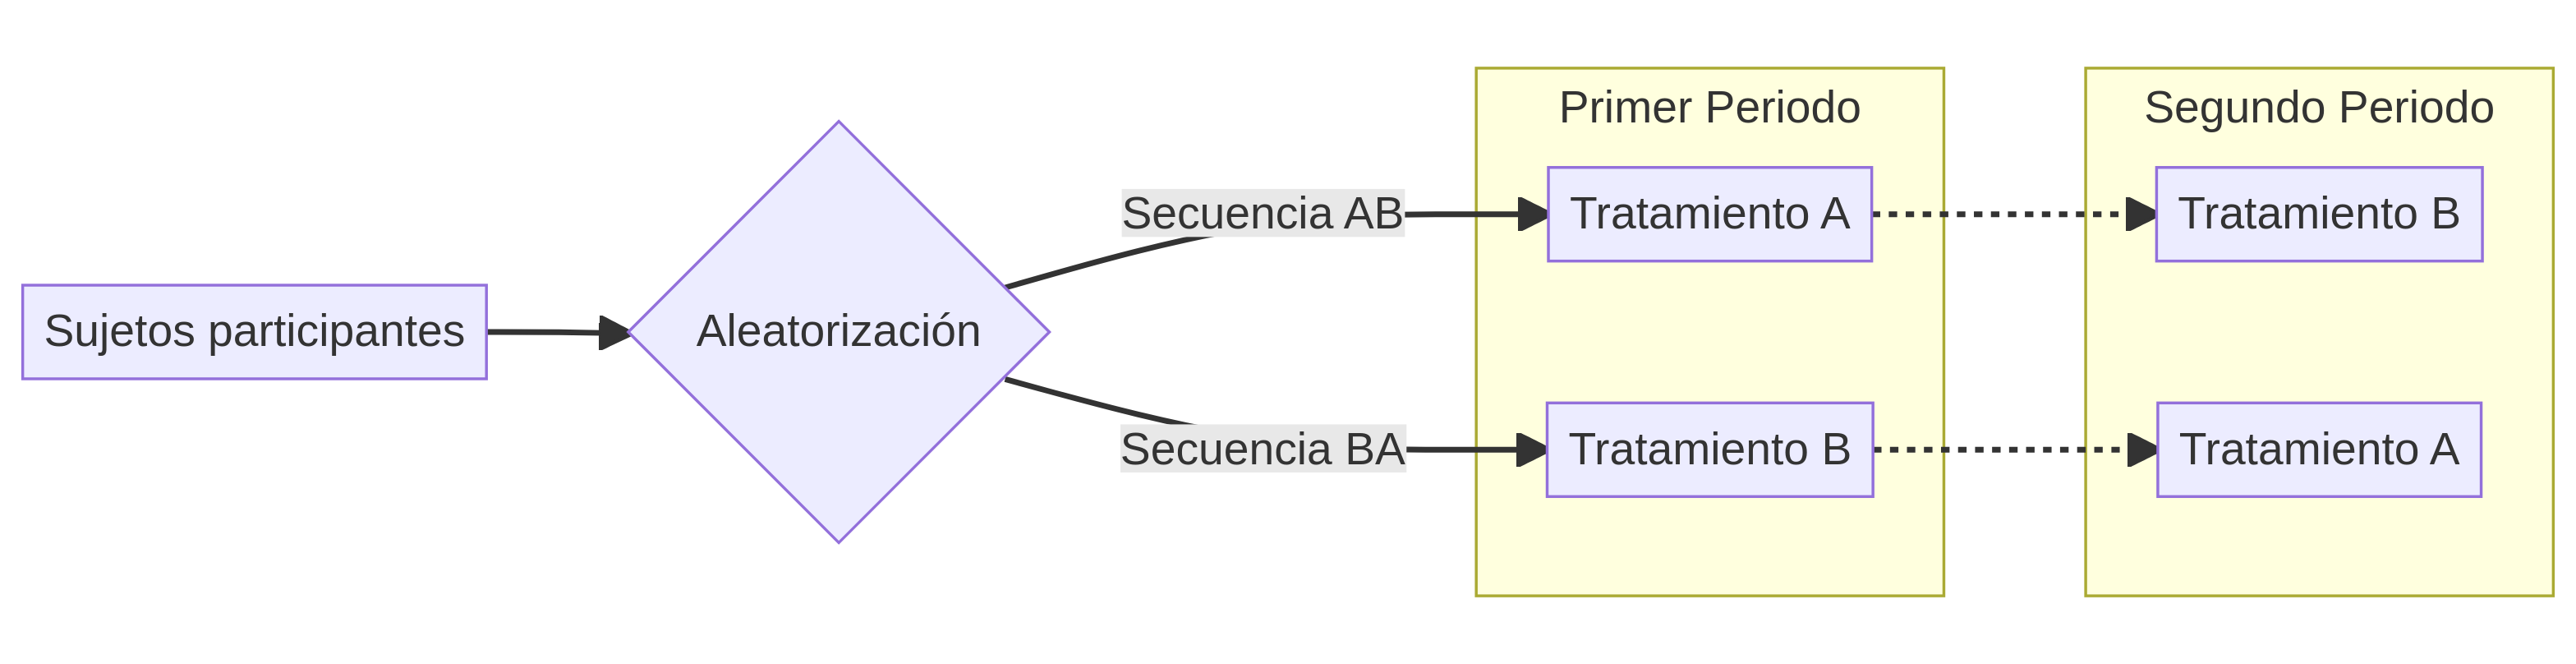
\includegraphics[width=6in,height=1.33in]{2_files/figure-latex/mermaid-figure-1.png}

}

\end{figure}

}

\caption{\label{fig-ab-ba}Diagrama de diseño cruzado AB/BA}

\end{figure}

\begin{figure}

{\centering 

\begin{figure}[H]

{\centering 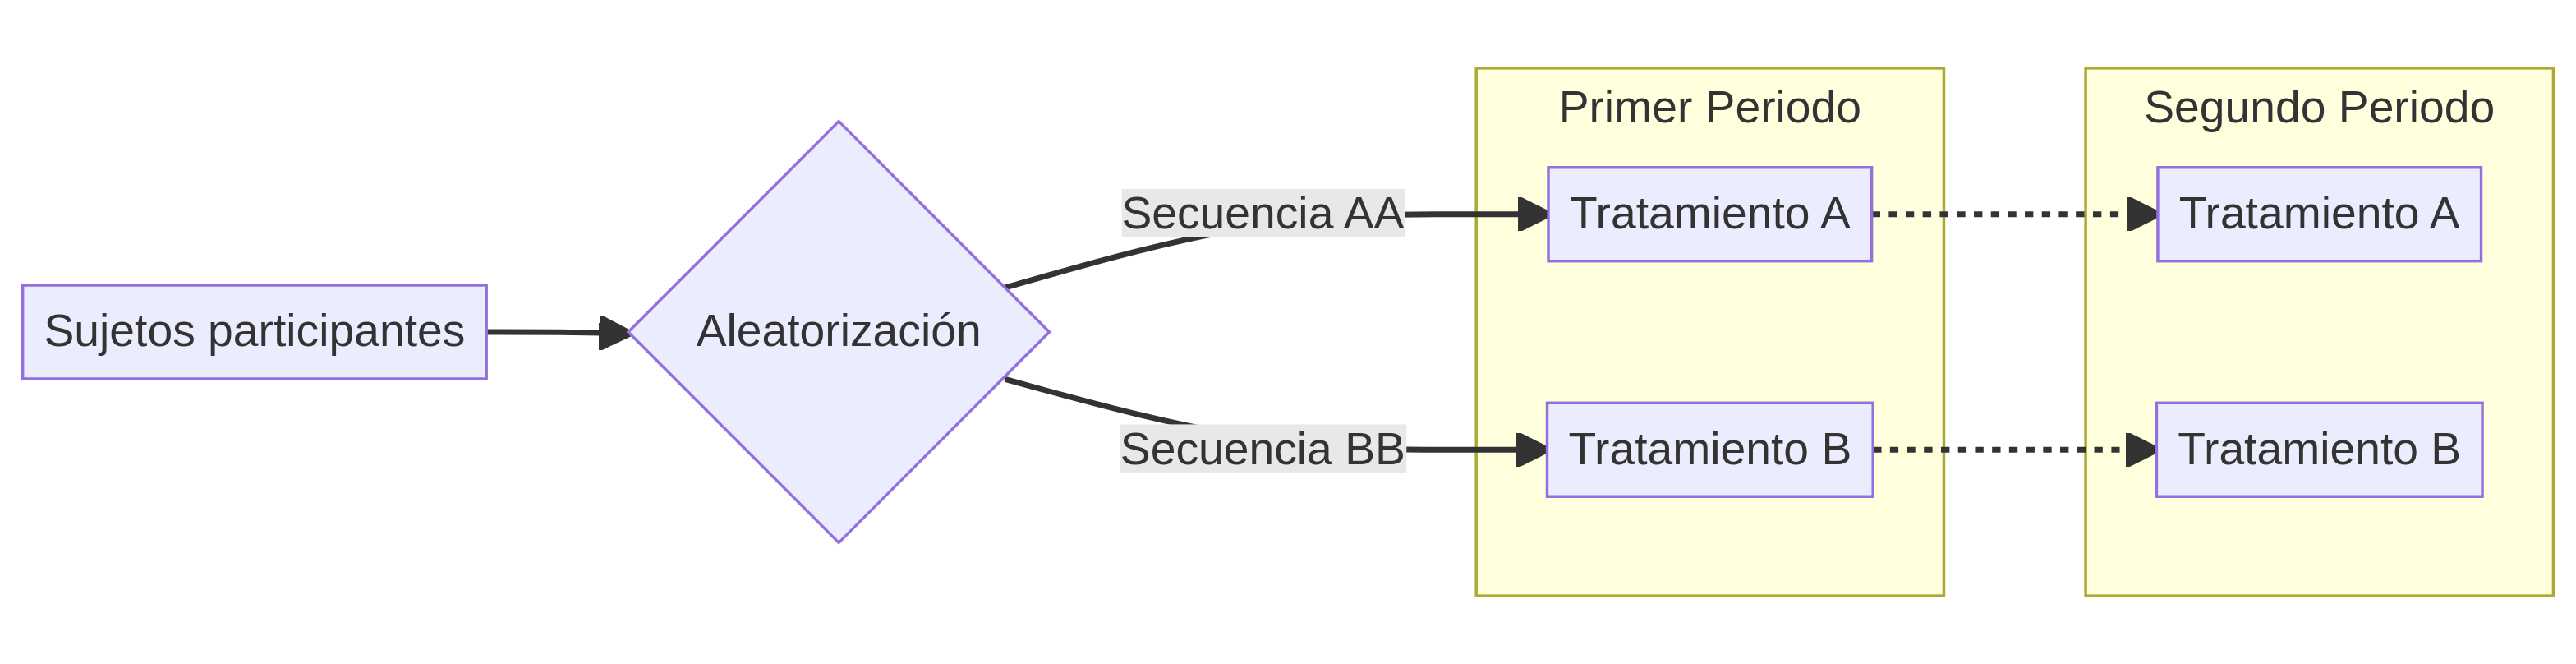
\includegraphics[width=6in,height=1.33in]{2_files/figure-latex/mermaid-figure-2.png}

}

\end{figure}

}

\caption{\label{fig-aa-bb}Diagrama de diseño paralelo AA/BB}

\end{figure}

Un \textbf{\gls{diseño completamente aleatorizado}}
\autocite[pp.~18]{lawson2015} \enquote{garantiza la validez del
experimento contra sesgos causados por otras variables ocultas. Cuando
las unidades experimentales se asignan aleatoriamente a los niveles de
factor de tratamiento, se puede realizar una prueba exacta de la
hipótesis de que el efecto del tratamiento es cero utilizando una prueba
de aleatorización}.

Siguiendo a \textcite[pp.~5-9]{senn2022}, para que el ensayo sea de tipo
cruzado no sería suficiente intercambiar las secuencias sino que debe
ser objeto del ensayo el estudio de las diferencias entre los
tratamientos individuales que componen las secuencias. Los principales
problemas de un diseño cruzado son el abandono, \texttt{drop-out}, de
alguno de los participantes y la interacción entre el tratamiento y el
periodo o \texttt{carry-over}. Además, el análisis estadístico es más
complicado, particularmente cuando la respuesta es ordinal y hay más de
dos tratamientos. En la misma línea, \textcite[pp.~1-2]{lui2016} afirma
que \enquote{el objetivo principal de un diseño cruzado es estudiar las
diferencias entre tratamientos individuales (en lugar de las diferencias
entre secuencias de tratamiento). Debido a que cada paciente sirve como
su propio control, el diseño cruzado es una alternativa útil al diseño
de grupos paralelos para aumentar la potencia}.

En un diseño cruzado pueden producirse efectos periodo y secuencia (o
\texttt{carry-over}). El \textbf{efecto periodo} aplicado al experimento
del subtitulado, se producirá si las respuestas del segundo periodo
están influidas por haber realizado la primera actividad de subtitulado.
El \textbf{efecto secuencia} se producirá si las respuestas fueran
diferentes cuando se realizan en un orden que cuando se realizan en el
otro. Como ejemplo de estos efectos se puede ver
\textcite[pp.~35-53]{senn2022}. Se analiza un experimento que consistió
en medir el flujo espiratorio máximo (PEF, por sus siglas en inglés) en
13 niños con edades entre los 7 y los 14 años con asma a los que se les
administró salbutamol (un conocido broncodilatador) y formoterol (un
broncodilatador de reciente aparición en el momento en que se realizó el
estudio). Se hicieron dos grupos a los que se les administró ambos
tratamientos en orden inverso dejando un periodo de lavado
(\texttt{washout\ period}) entre aplicaciones. El \gls{efecto periodo}
resulta de medir si el PEF medio de los dos grupos es diferente entre
periodos, y el \gls{efecto secuencia} consiste en comprobar si hay
diferencias significativas entre aplicar primero el tratamiento con
salbutamol y luego con formoterol o hacerlo al revés.

La segunda cuestión de relevancia es que las respuestas a los ítems de
una \gls{escala de likert} son de \textbf{tipo ordinal}. Los test
estadísticos \emph{\gls{ANOVA}} o \emph{\gls{MANOVA}} presuponen que la
variable de respuesta es cuantitativa y con distribución normal. Tratar
las respuestas a una escala de Likert como si fueran cuantitativas no es
correcto por las siguientes razones:

\begin{itemize}
\item
  Los niveles de respuesta no son necesariamente equidistantes: la
  distancia entre cada par de opciones de respuesta correlativos puede
  no ser la misma para todos los pares. Por ejemplo, la diferencia entre
  \enquote{Muy en desacuerdo} y \enquote{En desacuerdo} y la diferencia
  entre \enquote{De acuerdo} y \enquote{Muy de acuerdo} es de un nivel,
  pero psicológicamente puede ser percibida de forma diferente por cada
  sujeto.
\item
  La distribución de las respuestas ordinales puede ser no normal. En
  particular esto sucederá si hay muchas respuestas en los extremos del
  cuestionario.
\item
  Las varianzas de las variables no observadas que subyacen a las
  variables ordinales observadas pueden diferir entre grupos,
  tratamientos, periodos, etc.
\end{itemize}

En \textcite{kruschke2018} se han analizado los problemas potenciales de
tratar datos ordinales como si fueran cuantitativos constatando que se
pueden presentar las siguientes situaciones:

\begin{itemize}
\tightlist
\item
  Se pueden encontrar diferencias significativas entre grupos cuando no
  las hay: \gls{error de tipo I}.
\item
  Se pueden obviar diferencias cuando en realidad sí existen:
  \gls{error de tipo II}.
\item
  Incluso se pueden invertir los efectos de un tratamiento.
\item
  También puede malinterpretarse la interacción entre factores.
\end{itemize}

Otra cuestión que hay que tener en cuenta es que, al tratarse de un
diseño cruzado, es de \textbf{medidas repetidas} ya que cada sujeto
realiza dos veces el test, uno con cada vídeo y que, por lo tanto, las
respuestas a cada test de un mismo sujeto no es independiente. Además,
tampoco se pueden considerar independientes los ítems que componen el
test ya que los ítems pretenden medir la misma variable latente: la
calidad del subtitulado.

En este trabajo se analiza si el nivel de subtitulado (correcto o
defectuoso) influye en el nivel de respuesta a los ítems de la escala de
Likert, que es la variable respuesta. Se evalua también la existencia de
efectos secuencia y periodo y la influencia que tienen sobre el nivel de
respuesta el estudiante y el propio ítem.

\hypertarget{sec-glm}{%
\section[Modelos Lineales Generalizados ]{\texorpdfstring{Modelos
Lineales Generalizados
\footnote{No se deben confundir los Modelos Lineales Generales con los
  Modelos Lineales Generalizados. En los primeros, también llamados
  Modelos de Regresión Multivariante, se presupone que la variable
  respuesta tiene una relación lineal con los predictores y sus valores
  se distribuyen normalmente. Los segundos son una generalización de los
  primeros y permiten que la variable respuesta admita otras
  distribuciones además de la normal.}}{Modelos Lineales Generalizados }}\label{sec-glm}}

El Modelo Lineal Generalizado (\emph{Generalized Linear Model}, \(GLM\))
es un modelo en el que la variable respuesta no sigue una distribución
Normal. Para especificar un \gls{GLM} son necesarios tres componentes
\autocite[ver][pp.~66-67]{agresti_2018}:

\begin{itemize}
\item
  Un componente aleatorio que será una distribución de probabilidad de
  la familia exponencial. Se asume que la variable respuesta \(Y\) se
  distribuye según este componente aleatorio.
\item
  Un componente lineal de predictores. \[
  \alpha+\beta_1x_1+...+\beta_px_p
  \]
\item
  Una función de enlace \(g\) que relaciona \(\mu=E(Y)\) con los
  predictores, de tal forma que: \[
  g(\mu)=\alpha+\beta_1x_1+...+\beta_px_p
  \]
\end{itemize}

La estimación de coeficientes en \emph{GLM} se realiza maximizando la
función de verosimilitud (\emph{Maximum Likelihood Estimation},
\emph{\gls{MLE}}). Es decir, que los coeficientes del modelo son
aquellos que maximizan la probabilidad de los datos.

\hypertarget{sec-logistica}{%
\subsection{Regresión Logística}\label{sec-logistica}}

La \gls{Regresión Logística} es un caso particular de \(GLM\) en el que
la variable respuesta es dicotómica. Aunque la Regresión Logística no es
aplicable directamente en las respuestas a una escala de Likert por ser
éstas ordinales, se introduce aquí por dos motivos:

\begin{itemize}
\tightlist
\item
  En la sección de modelado (ver Sección~\ref{sec-logistica-2}), se
  propondrá una transformación de la variable respuesta para convertirla
  en dicotómica.
\item
  Además, en este capítulo se introducirá la Regresión Ordinal (ver
  Sección~\ref{sec-ordinal}). Este modelo se puede considerar una
  extensión de la Regresión Logística y permitirá tratar la variable
  respuesta como ordinal. De ahí el interés en presentar previamente la
  Regresión Logística.
\end{itemize}

La \gls{Regresión Logística} \autocite[ver][pp.~68-69]{agresti_2018} es
un caso particular de \(GLM\) donde la variable respuesta, \(Y\), es
Benoulli o Binomial. Es decir, que \(Y\) toma valores 0 ó 1. En una
función de Bernoulli de parámetro \(\pi\) (\(E[Y] = P(Y=1) = \pi\)), es
necesaria una función que mapee los valores que puede tomar el
componente lineal de rango \((-\infty, +\infty)\) a los valores que
puede tomar \(\pi\) en el rango \((0, 1)\). Una función que permite
hacer esto es la \emph{\gls{función logit}}:

\begin{equation}\protect\hypertarget{eq-logistic}{}{
logit(Y=1) = log \left[\frac{P(Y=1)}{1-P(Y=1)} \right] = \alpha+\beta_1x_1+...+\beta_px_p
}\label{eq-logistic}\end{equation}

La inversa de la función \emph{logit} es la
\emph{\gls{función logística}} y permite realizar el mapeo inverso para
obtener la probabilidad:

\[
P(Y=1) = \frac{exp^{\alpha+\beta_1x_1+...+\beta_px_p}}{1 + exp^{\alpha+\beta_1x_1+...+\beta_px_p}}
\]

La interpretación de los coeficientes es la siguiente
\autocite[ver][p.~260]{frienly2015}:

\begin{itemize}
\tightlist
\item
  \(\alpha\) es el logaritmo del \emph{\gls{odds}} de \(Y\) cuando
  \(x_j=0, \forall j \in 1...p\).
\item
  \(\beta_j\) es el logaritmo del \emph{\gls{odds ratio}} asociado a una
  unidad de incremento de \(x_j\).
\end{itemize}

El contraste de hipótesis para los coeficientes \(\beta\):

\[
\begin{aligned}
H_0: \beta_j =  0 \\
H_1: \beta_j \ne  0
\end{aligned}
\]

se puede realizar con el Test de Wald:

\[
\begin{aligned}
W & = \frac{\hat\beta_j - 0}{se(\hat\beta_j)} \sim N(0,1)
\end{aligned}
\]

o con el Test de Razón de Verosimilitudes (\emph{Likelihood Ratio Test},
\emph{\gls{LRT}}):

\[
\begin{aligned}
LRT = \Lambda &= -2 \log \frac{L(\widehat{reducido})}{L(\widehat{completo})}\\
&= -2 \log L(\widehat{reducido}) + 2 \log L(\widehat{completo}) \sim \chi^2_r
\end{aligned}
\]

donde:

\begin{itemize}
\tightlist
\item
  r es el número de \(\beta's\) iguales a cero.
\item
  \(L(\widehat{reducido})\) es el valor que maximiza la función de
  verosimilitud en la que algunos de los \(\beta's\) han sido igualados
  a cero.
\item
  \(L(\widehat{completo})\) es el valor que maximiza la función de
  verosimilitud en el modelo que incluye todos los \(\beta's\).
\end{itemize}

\(LTR\) permite comprobar la hipótesis de que uno o varios coeficientes
sean cero. Para comparar modelos no anidados, se puede usar el Criterio
de Información de Akaike (AIC) o el Criterio de Información Bayesiano
(BIC), que se definen respectivamente:

\begin{equation}\protect\hypertarget{eq-aic}{}{
\begin{aligned}
AIC &: -2 \log L + 2p \\
BIC &: -2 \log L + p \log(n)
\end{aligned}
}\label{eq-aic}\end{equation}

donde \(L\) es el valor de maxima verosimilitud y el segundo sumando es
una penalización que será mayor cuanto más complejo sea el modelo
(\emph{p = número de parámetros}, \emph{n = observaciones}).

\hypertarget{sec-ordinal}{%
\subsection{Regresión Ordinal}\label{sec-ordinal}}

Las respuestas a los ítems de una escala de Likert son ordinales. La
\gls{Regresión Ordinal} es una clase de \(GLM\) que comparte muchas
similitudes con la Regresión Logística (ver Sección~\ref{sec-logistica})
pero que tiene en consideración que los valores de la variable de
respuesta están ordenados \footnote{Otras variantes de la Regresión
  Logística son la Regresión Categórica y la Regresión Multinomial. En
  estos tipos de \emph{GLM} la variable respuesta puede adoptar varios
  valores pero no se asume que estén ordenados. La Regresión Categórica
  y la Regresión Multinomial están relacionadas en el mismo sentido en
  que lo están la Regresión Logística con función de enlace Bernoulli y
  con función de enlace Binomial. Es decir, que la Regresión Categórica
  se usa cuando las observaciones no están agrupadas y la Multinomial
  cuando sí lo están.}. Según \textcite[pp.~3-11]{burkner2019} hay tres
clases de Regresión Ordinal:

\begin{itemize}
\tightlist
\item
  Regresión Ordinal Acumulativa.
\item
  Regresión Ordinal Secuencial.
\item
  Regresión Ordinal Adyacente.
\end{itemize}

Las regresiones ordinales secuencial y adyacente presuponen que para
alcanzar un nivel se ha tenido que pasar previamente por los anteriores.
En un ítem de Likert esto carece de sentido y, por lo tanto, se
descartan estos modelos y se prefiere el \emph{Modelo Acumulativo}
(\emph{Cumulative Model}, \(CM\)) que además es el más utilizado
\autocite[ver][pp.~23-24]{burkner2019}.

\(CM\) presupone que la variable ordinal observada, \(Y\), proviene de
la categorización de una variable latente (no observada) continua,
\(\tilde{Y}\). Hay \(K\) umbrales \(\tau_k\) que particionan
\(\tilde{Y}\) en \(K + 1\) categorías ordenadas observables (ver
Figura~\ref{fig-cumulative}). Si se asume que \(\tilde{Y}\) tiene una
cierta distribución (por ejemplo, normal) con distribución acumulada
\(F\), se calcula la probabilidad de que \(Y\) sea la categoría \(k\) de
esta forma:

\[Pr(Y = k) = F(\tau_k) - F(\tau_{k-1})\]

\begin{figure}[h]

{\centering 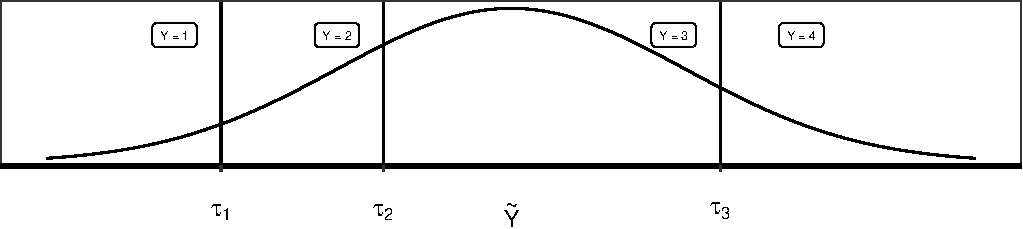
\includegraphics{2_files/figure-pdf/fig-cumulative-1.pdf}

}

\caption{\label{fig-cumulative}Función latente en una regresión ordinal
acumulativa.}

\end{figure}

Por ejemplo en la Figura~\ref{fig-cumulative}:
\(Pr(Y = 2) = F(\tau_2) - F(\tau_{1})\). Suponiendo que \(\tilde{Y}\)
tenga una relación lineal los predictores:

\[\tilde{Y} = \eta + \epsilon = \beta_1 x_1 + \beta_2 x_2 + ... + \beta_p x_p + \epsilon\]

entonces la función de probabilidad acumulada de los errores tendrá la
misma forma que la de \(\tilde{Y}\):

\[\mathrm{Pr}(\epsilon \leq z) = F(z)\]

Se puede calcular la distribución de probabilidad acumulada de \(Y\):

\[\mathrm{Pr}(Y \leq k \mid \eta) = \mathrm{Pr}(\tilde{Y} \leq \tau_k \mid \eta) = \mathrm{Pr}(\eta + \epsilon \leq \tau_k) = \mathrm{Pr}(\epsilon \leq \tau_k - \eta) = F(\tau_k - \eta)\]

Por lo que asumiendo la normalidad de los errores:

\[\mathrm{Pr}(Y = k) = \Phi(\tau_k - \eta) - \Phi(\tau_{k - 1} - \eta)\]

donde hay que estimar los umbrales y las pendientes de cada variable
explicativa. La función anterior es la conocida como la función de
enlace \texttt{probit}. La interpretación de los coeficientes con esta
función de enlace no resulta intuitiva. Por ello en este trabajo se va a
utilizar la función de enlace \texttt{logit}. Con esta función de enlace
la interpretación de los coeficientes es parecida a la de los
coeficientes de la regresión logística. Además, en la práctica, los
coeficientes estimados suelen tener valores similares a los de la
función \texttt{probit}. Para entender como se deben interpretar los
coeficientes del modelo \(CM\) se parte del supuesto de que el \(logit\)
de la función de probabilidad es lineal:

\begin{equation}\protect\hypertarget{eq-ordinal}{}{
logit [P(Y \le k)] = \tau_{k} - \eta = \tau_{k} - (\beta_1 x_1 + \beta_2 x_2 + ... + \beta_p x_p)
}\label{eq-ordinal}\end{equation}

En ese caso, se puede demostrar fácilmente que, por ejemplo:

\[\frac{\frac{\mathrm{Pr}(Y \leq k \mid \eta)}{\mathrm{Pr}(Y > k \mid \eta)}}{\frac{\mathrm{Pr}(Y \leq k+1 \mid \eta)}{\mathrm{Pr}(Y > k+1 \mid \eta)}} = \exp(\tau_{k} - \tau_{k+1})\]

Y que \footnote{En la Sección~\ref{sec-ordinal-2} se demuestra esta
  fórmula.}:

\[\frac{\frac{\mathrm{Pr}(Y \leq k \mid x_j = 1)}{\mathrm{Pr}(Y > k \mid x_j = 1)}}{\frac{\mathrm{Pr}(Y \leq k \mid x_j=0)}{\mathrm{Pr}(Y > k \mid x_j = 0)}} = \exp(-\beta_{j})\]

o, equivalentemente:

\[\frac{\frac{\mathrm{Pr}(Y > k \mid x_j = x + 1)}{\mathrm{Pr}(Y \leq k \mid x_j = x + 1)}}{\frac{\mathrm{Pr}(Y > k \mid x_j = x)}{\mathrm{Pr}(Y \leq k \mid x_j = x)}} = \exp(\beta_{j})\]

Es decir, que \(\exp(\beta_{j})\) es el \emph{odds ratio} (cambio
relativo entre \(odds\), \gls{OR}) de que la variable respuesta esté por
encima de una determinada categoría versus estar por debajo de ella para
una unidad de incremento del predictor \(x_j\). Un valor del coeficiente
\(\beta_j\) positivo indica que la relación entre el predictor \(x_j\) y
la función de \(logit\) es positiva y, por lo tanto, se incrementa la
probabilidad de un mayor valor de la variable respuesta.

\hypertarget{presunciones-del-modelo}{%
\subsubsection{Presunciones del modelo}\label{presunciones-del-modelo}}

Este modelo se denomina proporcional ya que se asume que cada predictor
tiene los mismos efectos sobre todos los niveles de la variable de
respuesta ordinal \autocite[ver][chap.~5]{Liu2202}. Es decir, que los
\(odds\) de los niveles de respuesta deben ser proporcionales para los
mismos valores de las variables explicativas. Esta suposición
frecuentemente no es realista y se puede relajar permitiendo estimar un
coeficiente diferente para cada nivel de la variable respuesta. Sin
embargo, el incremento del número de coeficientes dificulta la
interpretabilidad del modelo. \textcite{harrell2020} aboga por usar este
modelo incluso aunque la suposición de proporcionalidad no se cumpla:

\begin{quote}
\enquote{Ningún modelo se ajusta perfectamente a los datos, \ldots, la
aproximación ofrecida por el modelo \(CM\) sigue siendo bastante útil. Y
un análisis unificado del modelo \(CM\) es decididamente mejor que
recurrir a análisis ineficientes y arbitrarios de valores dicotomizados
de Y.}
\end{quote}

Matemáticamente la presunción de la proporcionalidad de los \(odds\) se
demuestra a partir de la Ecuación~\ref{eq-ordinal}. Si se fijan los
predictores en un valor arbitrario \(X=x\) y se consideran dos niveles
de respuesta cualesquiera \(k\) y \(l\), entonces:

\begin{equation}\protect\hypertarget{eq-ordinal2}{}{
\begin{aligned}
logit [P(Y \le k | X = x)] - logit [P(Y \le l | X = x)] = \tau_{k} - \tau_{l} \\
\frac{odds(P(Y \le k | X = x))}{odds(P(Y \le l | X = x))}  =  \exp(\tau_{k} - \tau_{l}) \implies \\
odds(P(Y \le k | X = x))  \propto odds(P(Y \le l | X = x))
\end{aligned}
}\label{eq-ordinal2}\end{equation}

Es decir, que la proporcionalidad de \(odds\) de dos niveles de
respuesta es independiente de los valores concretos de los predictores,
por lo que la constante de proporcionalidad debe ser similar para todos
ellos.

\hypertarget{sec-multinivel}{%
\section{Modelos multinivel}\label{sec-multinivel}}

Un modelo multinivel (\emph{\gls{GLMM}}, \emph{Ganeralized Linear Mixed
Model}ß), anidado, jerárquico o mixto es un modelo en el que los datos
están anidados en una estructura jerárquica. Se utilizan cuando se
incumple la hipótesis de independencia entre las observaciones. Por
ejemplo, si se quisiera evaluar el rendimiento de varios métodos de
enseñanza, se podrían seleccionar aleatoriamente varios colegios
participantes y en cada uno de ellos elegir varias clases en las que se
impartiría uno de los métodos de enseñanza. En este caso, los alumnos de
una clase no son independientes de los alumnos de otra clase del mismo
colegio y también es esperable que los alumnos de un mismo colegio sean
más parecidos entre sí que los de otro colegio. Otra situación en la que
se viola la condición de independencia entre observaciones es cuando se
toman varias medidas del mismo sujeto. Este tipo de experimentos se
llaman de medidas repetidas o longitudinales \footnote{Hay una
  diferencia conceptual entre medidas repetidas y longitudinales. Una
  variable se dice que es longitudinal cuando se toman varias medidas de
  los sujetos objeto del estudio en diferentes momentos del tiempo. Para
  que sea considerada de medidas repetidas, las medidas de cada sujeto
  se toman con distintos niveles de factor. En la práctica la distinción
  es poco relevante ya que ambas situaciones se parametrizan de la misma
  forma.}. Cuando se da este supuesto, se considera que las medidas
están anidadas en el sujeto \autocite[ver][]{Liu2202}. En un modelo
multinivel no es necesario que todas las variables tengan una estructura
jerárquica. Se distinguen entonces dos tipos de variables: Las conocidas
como de efectos fijos son aquellas que se considera que tienen el mismo
efecto en toda la población y, por lo tanto, se debe estimar un único
coeficiente. Las variables de efectos aleatorios tienen un coeficiente
diferente para cada elemento de la población y se supone que son una
muestra de una población mucho mayor, como el caso de seleccionar
aleatoriamente una muestra de colegios. Normalmente el coeficiente
particular de cada elemento no es de interés para el investigador y se
asume que tienen una media centrada en cero. El mayor interés de los
efectos aleatorios es la estimación de su matriz de
varianzas-covarianzas.

La ecuación general de un modelo multinivel con dos niveles y un solo
predictor con efectos aleatorios es \autocite[ver][pp.~40]{chen2021}:

\[
\begin{aligned}
Nivel\ 1: & y_{ij}     & = & \beta_{0j} + \beta_{1j}x_{1ij} + \epsilon_{ij} \\
Nivel\ 2: & \beta_{0j} & = & \beta_{0} + U_{0j} & (intercepto\ aleatorio) \\
          & \beta_{1j} & = & \beta_{1} + U_{1j} & (pendiente\ aleatoria) \\
\end{aligned}
\]

Los errores del modelo se distribuyen:

\[
\begin{aligned}
\text{Error intra grupo: } &  \epsilon_{ij} \sim N(0, \sigma^2) \\
\text{Error entre grupos: } &
\begin{pmatrix}
     U_{0j} \\
     U_{1j} \\
\end{pmatrix} 
\sim
N
\begin{pmatrix}
\begin{pmatrix}
     0 \\
     0 \\
\end{pmatrix},
\begin{pmatrix}
     \tau_0^2 & \tau_0\tau_1\rho_{01} \\
     \tau_0\tau_1\rho_{01} &  \tau_1^2 \\
\end{pmatrix}
\end{pmatrix} 
\end{aligned}
\]

donde \(j\) son los grupos que varían \(j = 1,...,J\) (\(J\) es el
número de grupos); \(ij\) es la observación \(i\)-ésima del grupo \(j\)
(\(i = 1,...,n_j\), \(n_j\) es el número de observaciones del grupo
\(j\)). El modelo se compone de una parte fija
\(\beta_0 + \beta_1 x_{1ij}\) y una aleatoria
\(U_{0j} + U_{1j} x_{1ij} + \epsilon{ij}\). Los parámetros de este
modelo son el intercepto y la pendiente de efectos fijos (\(\beta_0\) y
\(\beta_1\)), la varianza intra-grupos (\(\sigma^2\)), la varianza
inter-grupos del intercepto aleatoria (\(\tau_0\)) y de la pendiente
aleatoria (\(\tau_1\)), y la correlación entre intercepto y pendiente
aleatorias (\(\rho_{01}\)).

En \textcite[p.~115]{gelman2013} se evalúan tres posibilidades a la hora
de definir un modelo:

\begin{itemize}
\tightlist
\item
  \(Complete\ pooling\): Consiste en estimar un único parámetro para
  cada predictor. Es equivalente a un modelo con efectos fijos.
\item
  \(No\ pooling\): Se estiman tantos parámetros como grupos haya de
  forma independiente.
\item
  \(Partial\ pooling\): Es el modelo jerárquico. Es una mezcla de ambos,
  ya que, aunque se estima un parámetro para cada grupo (como en
  \(no\ pooling\)), esta estimación no es independiente, sino que se
  supone que las observaciones de un mismo grupo proceden de una misma
  distribución de probabilidad. Esto se traduce en que se produce una
  contracción (\emph{\gls{shrinkage}}) en la estimación de los
  parámetros hacia la media. Al influir la estimación de unas
  observaciones en otras, la estimación es de menor valor absoluto que
  la que resultaría en un modelo de \(no\ pooling\). De esta forma se
  puede ver el \(complete\ pooling\) y el \(no\ pooling\) como dos casos
  particulares y extremos del \(partial\ pooling\). La contracción de
  coeficientes en los modelos multinivel actúa como una regularización
  que puede evitar el sobreajuste.
\end{itemize}

Los modelos multinivel requieren supuestos adicionales en el nivel
segundo y superiores que son similares a los supuestos para los modelos
de efectos fijos \autocite[ver][p.~43]{chen2021}. Para estimar los
parámetros en un modelo multinivel se suele utilizar el método de Máxima
Verosimilitud Restringida (\(RMLE\)), que es una variante de la
estimación por Máxima Verosimilitud (\(MLE\)) en la que se hacen ajustes
en los grados de libertad del modelo con efectos aleatorios para
corregir el sesgo que se produce al usar \(MLE\) en estos modelos.

Para evaluar si la estructura anidada es adecuada se utiliza la
Correlación Intra-Clase (\emph{\gls{ICC}}, Intra-Class Correlation).
\(ICC\) se puede interpretar como la proporción de la varianza explicada
por la estructura de agrupamiento de la población. Se diferencia del
Coeficiente de Determinación (\(R2\)) en que éste es la proporción de la
varianza explicada por el modelo completo, mientras que \(ICC\) es la
varianza explicada por los efectos aleatorios
\autocite[ver][]{performance}. La \(ICC\) se calcula como el ratio de la
varianza entre grupos y la varianza total
\autocite[ver][pp.~29-33]{chen2021}:

\[
ICC = \rho = \frac{\tau^2}{\tau^2+\sigma^2}
\]

donde \(\tau^2\) es la varianza poblacional entre grupos y \(\sigma^2\)
es la varianza de la población dentro del grupo. \(ICC\) oscila entre 0
(ausencia de varianza entre grupos) y 1 (no varianza intra-grupos).
Cuanto más proxima a 1 sea \(ICC\) mayor evidencia hay de la existencia
de una estructura anidada. Sin embargo, no hay un consenso sobre el
umbral concreto que debe tener \(ICC\) para decidir si es preferible o
no la estructura anidada \autocite[ver][p.~33]{chen2021}. \(ICC\) se
estima a partir de la varianza de los coeficientes y residual aleatorias
calculadas por el modelo. En modelos \(GLM\) no se calcula la varianza
residual y se recurre a métodos de simulación para estimar \(ICC\).

\hypertarget{sec-bayesiano}{%
\section{Modelado bayesiano}\label{sec-bayesiano}}

El paradigma frecuentista parte de la suposición de que los datos son
generados a partir de una variable aleatoria \(Y\) y para estimar los
coeficientes se maximiza la función de verosimilitud \(p(y | \theta)\)
que depende del parámetro desconocido \(\theta\). En el análisis
bayesiano se considera que \(\theta\) es una variable aleatoria ya que
hay incertidumbre respecto a su valor. Esto se traduce en que se debe
asignar una distribución de probabilidad \(p(\theta)\), conocida como
distribución a priori, que expresa nuestra creencia sobre los valores
que puede tomar \(\theta\). En la inferencia bayesiana se usa la
distribución de probabilidad a posteriori \(p(\theta | y)\) que es
proporcional al producto de la función de verosimilitud y de la
distribución de probabilidad a priori \autocite[ver][]{nicenboim2023}:

\[
\hbox{Posterior} = \frac{\hbox{Likelihood} \times \hbox{Prior}}{\hbox{Marginal Likelihood}}
\Rightarrow p(\theta|y) = \cfrac{ p(y|\theta) \times p(\theta) }{p(y)} \propto p(y|\theta) \times p(\theta)
\]

En la inferencia bayesiana hay dos fuentes de incertidumbre: Por un lado
hay que contar con la variabilidad de \(Y\), ya que si se toman varias
muestras, los valores \(y_i\) obtenidos serán diferentes. Además, existe
otra incertidumbre que proviene del desconocimiento del valor de
\(\theta\). En la estimación frecuentista, debido a que se utilizan
estimaciones puntuales de \(\theta\), no se tiene en cuenta esta
incertidumbre. La Ecuación~\ref{eq-ypred} se corresponde con la
distribución predictiva a posteriori que tiene en consideración ambas
incertidumbres: \begin{equation}\protect\hypertarget{eq-ypred}{}{
\begin{aligned}
p(y_{pred}\mid y ) & = \int_{\theta} p(y_{pred}, \theta \mid y)\, d\theta= \int_{\theta} 
p(y_{pred}\mid \theta,y)p(\theta \mid y)\, d\theta \\ 
& = \int_{\theta} p(y_{pred}\mid \theta) p(\theta \mid y)\, d\theta
\end{aligned}
}\label{eq-ypred}\end{equation}

donde la última igualdad resulta de la independencia condicional de
\(y_{pred}\) e \(y\) dado \(\theta\)
(\(y_{pred} \perp\!\!\!\perp y \mid \theta\)).

Una crítica habitual a la inferencia bayesiana es que la elección de la
distribución de probabilidad a priori es subjetiva. Aunque es cierto que
hay un grado de subjetividad en esta elección, en realidad en el
modelado frecuentista hay que tomar ciertas decisiones que también lo
son, como por ejemplo la elección del nivel de significación o la forma
que adopta la función de verosimilitud. En la práctica, si las
observaciones son suficientemente informativas y la distribución a
priori es poco informativa, la distribución de probabilidad a priori
tendrá poca o nula influencia en la distribución a posteriori ya que
estará dominada por la función de verosimilitud y los coeficientes
estimados serán muy parecidos en ambos paradigmas. Sin embargo, en lo
que diferirán es en la interpretación ya que, por ejemplo, en un modelo
bayesiano se pueden interpretar los intervalos de confianza como la
probabilidad de que el parámetro esté dentro del intervalo. Por eso a
estos intervalos se les conoce como intervalos de credibilidad. Esa
interpretación en un modelo frecuentista carecería de sentido ya que los
parámetros del modelo no se consideran variables aleatorias y, por lo
tanto, tendrán probabilidad 1 si el verdadero valor del parámetro cae
dentro del intervalo y 0 si no lo hace. Para obtener la distribución de
probabilidad a posteriori normalmente se recurre a métodos del
simulación Métodos de Montcarlo basados en Cadenas de Márkov
(\emph{\gls{MCMC}}). \footnote{En ocasiones se puede obtener una forma
  análitica de la distribución a posteriori si se elige una adecuada
  combinación de función de verosimilitud y distribución a priori
  conocidas como distribuciones conjugadas. Aunque esto evita la
  utilización de métodos de simulación, restringe las formas posibles de
  las distribuciones. En la actualidad, con el aumento de la capacidad
  de cálculo de los ordenadores, normalmente no es necesaria la
  utilización de distribuciones conjugadas.}.

Para comparar modelos entre sí se pueden usar varias medidas
\autocite[ver][]{barreda2023}. Por ejemplo, la conocida como \emph{log
pointwise predictive density} o densidad predictiva puntal (\(lpd\)) se
calcula como: \[
\widehat{\mathrm{lpd}} = \sum_{i=1}^{N} \mathrm{log} (p(y_{i} | \theta))
\]

La \(lpd\) es la densidad conjunta de observar los datos dada la
estructura del modelo y las estimaciones de los parámetros \(\theta\).
Aunque las probabilidades a priori no se incluyen en su cálculo, sí
influyen en la estimación de \(\theta\) y, por lo tanto, tienen un
efecto en los valores de \(lpd\). Mayores valores de \(lpd\) estarían
indicando un mejor modelo. El problema con esta métrica es que se
utilizan los datos tanto para estimar el modelo como para seleccionar el
mejor modelo. Esto va a producir un sobreajuste y tenderá a favorecer
los modelos más complejos. Una métrica mejor es la \emph{expected log
pointwise predictive density} o densidad predictiva puntual esperada
(\(elpd\)). Se define en términos de valores fuera de la muestra
\(\tilde{y}\) en lugar de con los valores de la muestra \(y\):

\[
\mathrm{elpd} = \sum_{i=1}^{N} \mathbb{E}(\mathrm{log} (p(\tilde{y}_i | \theta)))
\]

En la práctica no se puede saber el valor de \(elpd\) ya que no se
conoce el proceso que genera verdaderos valores \(\tilde{y}\). Una forma
de estimar \(elpd\) que empíricamente se ha demostrado que funciona es
penalizar \(lpd\) con el número de parámetros \(p\) de forma análoga a
lo que se hace en \(AIC\) (ver Ecuación~\ref{eq-aic}):

\[
\widehat{\mathrm{elpd}} = \widehat{\mathrm{lpd}} - \mathrm{p}
\]

El problema es que en modelos multinivel conocer el número de parámetros
no es sencillo ya que los parámetros asociados a efectos aleatorios no
se pueden considerar que sean completamente independientes. El número
efectivo de parámetros va a depender de la importancia de la regresión
hacia la media que sufra cada parámetro. Además, en lugar de usar una
estimación puntual, se puede utilizar toda la distribución de valores de
la simulación. La métrica \emph{widely available information criterion}
o \enquote{criterio de información ampliamente disponible} (\(WAIC\)) es
una forma de estimar \(lpd\) que usa toda la distribución de
probabilidad a posteriori:

\[
\widehat{\mathrm{lpd}} = \sum_{i=1}^{n} \mathrm{log} (\frac{1}{S} \sum_{s=1}^{S} p(y_{i} | \theta^s))
\]

donde \(S\) es el tamaño de la muestra y el sumatorio interior es la
media de densidad en un punto \(i\). Para penalizar los modelos más
complejos, se usa la varianza de la función de densidad logarítmica:

\[
\begin{aligned}
\widehat{\mathrm{elpd}}_{WAIC} &= \widehat{\mathrm{lpd}} - \mathrm{p_{WAIC}} \\
\mathrm{p_{\mathrm{WAIC}}} &= \sum_{i=1}^{n} \mathrm{Var}_{s=1}^{\,S}(\mathrm{log} (p(y_{i} | \theta^s)))
\end{aligned}
\]

Una forma alternativa de evaluar un modelo es mediante validación
cruzada (\(CV\), Cross Validation). La validación cruzada más popular es
\emph{K-fold-CV}. Con esta técnica se divide el conjunto de datos en
\(K\) partes y se entrena el modelo separando sucesivamente cada una de
las partes que se usan para evaluar el modelo. Los valores estimados
resultan de promediar los \(K\) resultados. El problema es que cuanto
menor sea \(K\) más inestables son los resultados obtenidos, y cuanto
menor sea \(K\) más veces hay que reentrenar el modelo. Un caso extremo
de validación cruzada, que produce gran estabilidad en las estimaciones,
es dejar un dato fuera cada vez (\emph{Leave One Out}, \(LOO\), \(K\) =
\(N\)). La dificultad es que requiere estimar el modelo tantas veces
como datos se tengan. Para evitar esto, hay formas de aproximar
\(\widehat{\mathrm{elpd}}\) basadas en \(LOO\) sin tener que reentrenar
el modelo. La fórmula es la siguiente:

\[
\begin{aligned}
\widehat{\mathrm{elpd}}_{LOO} \approx \sum_{i=1}^{n} \mathrm{log} (p(y_{i} | \theta_{y_{-i}}))
\end{aligned}
\]

donde \(\theta_{y_{-i}}\) es la estimación de \(\theta\) que resulta
tras eliminar la observación \(y_{i}\) \autocite[ver][
pp.~175-176]{gelman2013}.

\bookmarksetup{startatroot}

\hypertarget{sec-metodo}{%
\chapter{Materiales y métodos}\label{sec-metodo}}

En este capítulo se describen los ficheros de datos suministrados, se
explica la tarea de preprocesado realizada sobre ellos y las variables
que se han utilizado en el modelado estadístico.

\hypertarget{ficheros-suministrados}{%
\section{Ficheros suministrados}\label{ficheros-suministrados}}

Se dispuso de los siguientes ficheros \texttt{csv}:

\begin{itemize}
\tightlist
\item
  Fichero \texttt{grade} contiene el identificador de estudiante y el
  grupo al que pertenece (campo \texttt{cohort}), ofuscado con
  \gls{sha}-512 para no conocer la identidad real del estudiante y con
  \gls{crc}-32b para no conocer si el grupo es el que el vio primero el
  vídeo bien subtitulado.
\item
  Los ficheros \texttt{test1} y \texttt{test2} son las repuestas a las
  escalas de Likert sobre la calidad del subtitulado del primer y del
  segundo vídeo realizado por cada grupo respectivamente.
\end{itemize}

En la Tabla~\ref{tbl-likert-levels} se muestran los 5 niveles de cada
uno de los ítems de la \gls{escala de likert} utilizados para valorar el
subtitulado \footnote{En la codificación original los valores asignados
  a cada respuesta eran diferentes: la opción \enquote{No sé / No
  contesto} se codificó con 5 y las demás opciones con una unidad menos
  que la mostrada. En este trabajo se ha hecho una rotación para asignar
  valores más usuales en la literatura científica sobre el tema.}. En la
Tabla~\ref{tbl-likert-scale} se muestran los 18 ítems de la escala de
Likert que se propuso a los alumnos para que evaluaran cada uno de los
vídeos.

\hypertarget{tbl-likert-levels}{}
\begin{longtable}[]{@{}rl@{}}
\caption{\label{tbl-likert-levels}Niveles de los ítems de la escala de
Likert.}\tabularnewline
\toprule\noalign{}
values & levels \\
\midrule\noalign{}
\endfirsthead
\toprule\noalign{}
values & levels \\
\midrule\noalign{}
\endhead
\bottomrule\noalign{}
\endlastfoot
0 & No sé / No contesto \\
1 & Muy en desacuerdo \\
2 & En desacuerdo \\
3 & Neutral \\
4 & De acuerdo \\
5 & Muy de acuerdo \\
\end{longtable}

\hypertarget{tbl-likert-scale}{}
\begin{longtable}{ll}
\caption{\label{tbl-likert-scale}Ítems de la escala de Likert. }\tabularnewline

\toprule
Item & Texto \\ 
\midrule
Q01 & La posición de los subtítulos \\ 
Q02 & El número de líneas por subtítulo \\ 
Q03 & La disposición del texto respecto a la caja donde se muestran los subtítulos \\ 
Q04 & El contraste entre los caracteres y el fondo \\ 
Q05 & La corrección ortográfica y gramatical \\ 
Q06 & La literalidad \\ 
Q07 & La identificación de los personajes \\ 
Q08 & La asignación de líneas a los personajes en los diálogos \\ 
Q09 & La descripción de efectos sonoros \\ 
Q10 & La sincronización de las entradas y salidas de los subtítulos \\ 
Q11 & La velocidad de exposición de los subtítulos \\ 
Q12 & El máximo número de caracteres por línea \\ 
Q13 & La legibilidad de la tipografía \\ 
Q14 & La separación en líneas diferentes de sintagmas nominales, verbales y preposicionales \\ 
Q15 & La utilización de puntos suspensivos \\ 
Q16 & La escritura de los números \\ 
Q17 & Las incorrecciones en el habla \\ 
Q18 & Los subtítulos del vídeo cumplen en general con los requisitos de accesibilidad \\ 
\bottomrule
\end{longtable}

\hypertarget{sec-preprocesado}{%
\section{Preprocesado}\label{sec-preprocesado}}

Los datos personales de los estudiantes se suministraron anonimizados
para evitar conocer su identidad. De acuerdo con el compromiso ético del
Canal, del estudio se han eliminado 19 estudiantes que, a pesar de haber
realizado la actividad, no dieron su consentimiento para que sus datos
se utilizaran en estudios científicos. Tras este proceso, se dispone de
198 cuestionarios correspondientes a 111 alumnos. Hay 24 estudiantes que
sólo realizaron el primero de los test. Como la muestra es
suficientemente amplia, se ha decidido eliminar estos test quedando 87
estudiantes participantes. De estos, 46 manifestaron tener sexo
femenino, 19 masculino y el resto (22) prefirieron no suministrar esta
información. Se constata que hay un claro sesgo hacia el sexo femenino
entre los participantes en la actividad de subtitulado.

En esta sección se describen las transformaciones realizadas con los
ficheros suministrados:

\begin{itemize}
\item
  Se leyó el fichero \texttt{grade}. El número de fila con el que el
  estudiante aparece en el fichero se utilizó como identificador del
  estudiante para mantener la trazabilidad y comprobar que las
  transformaciones realizadas son correctas.
\item
  Se eliminaron los datos de los estudiantes que, aun habiendo realizado
  la actividad, no dieron su consentimiento para participar en el
  estudio.
\item
  El valor del campo \texttt{cohort}, que se indica el valor anonimizado
  para el grupo, se sustituyó por una letra, \(A\) o \(B\). En el
  momento en que se realizó este proceso se desconocía qué vídeo vio
  primero cada cohorte.
\item
  Se leyeron los ficheros de test y se procesaron. Se utilizó el nombre
  del fichero (\texttt{test1} o \texttt{test2}) para saber de qué vídeo
  se estaba respondiendo el test \footnote{Se reitera que en el momento
    de realizar este proceso se desconocía si el vídeo es el
    correctamente subtitulado o el otro. La única información que se
    almacenó es si se estaba respondiendo al vídeo que se vio primero.}.
\item
  Se seleccionaron los ítems que contienen las respuestas y se
  renombraron para que fuera más fácil saber de qué ítem se trataba
  \footnote{En los ficheros suministrados la respuesta a cada ítem
    ocupaba varios campos. Se seleccionó en cada ítem el que contiene el
    valor de la respuesta y se convirtió a numérico.}. Se convirtió el
  campo \texttt{LastTry}, que contiene la fecha y hora de realización
  del test, a formato fecha y hora.
\item
  Se realizaron algunas comprobaciones como la ausencia de valores nulos
  en las variables más relevantes y la no existencia de inconsistencias
  o errores de procesado.
\item
  Se eliminaron los comentarios y se grabaron en fichero aparte para que
  no revelaran información que habría podido descubrir el tipo de
  subtitulado que piensa que estaba evaluando el estudiante.
\item
  Se renombraron las variables (ver Tabla~\ref{tbl-variables}).
\item
  Se eliminaron del estudio los estudiantes que solo han realizado uno
  de los test.
\item
  Se transformaron las variables que lo requirieron en factores. El ítem
  18 se fijó como referencia en el factor \texttt{Item} ya que es una
  valoración general del subtitulado.
\item
  Se rotaron los valores de respuesta para que \enquote{No sé / No
  contesto} tenga valor 0 y el resto de 1 a 5 desde \enquote{Muy en
  desacuerdo}, 1, hasta \enquote{Muy de acuerdo}, 5.
\item
  Se crearon los factores \texttt{Level} con los niveles
  \texttt{negativo}, \texttt{neutral} y \texttt{positivo} dependiendo de
  si la respuesta es 1 ó 2, 3, 4 ó 5 respectivamente e \texttt{Improve}
  con valores 0 ó 1, dependiendo de si la respuesta en el test \(A\) es
  mejor (1) o igual o peor (0) que la del \(B\) para cada ítem y
  estudiante.
\item
  Se transformó el \texttt{dataframe} de formato ancho a largo. Los
  ficheros de respuestas originales se suministraron en formato ancho.
  Es decir, que cada fila es un test que contiene 18 columnas para las
  respuestas a cada ítem. Los nombres de las columnas son \(Q01\),
  \(Q02\), \ldots, \(Q18\) y tienen valores de 0 a 5 con las respuestas.
  La mayoría de los paquetes de R utilizados requieren que los datos
  estén en formato largo. Esto que quiere decir que cada fila tendrá una
  única respuesta por lo que habrá únicamente dos columnas, \(Item\) y
  \(Response\). En la primera se almacena el identificador del ítem
  (\(Q01\), \(Q02\), \ldots, \(Q18\)) y en la segunda el valor de la
  respuesta (de 0 a 5). De esta forma, un test pasó de ocupar una fila y
  18 columnas en el formato ancho a 18 filas y dos columnas en el largo.
\end{itemize}

\hypertarget{variables-utilizadas}{%
\section{Variables utilizadas}\label{variables-utilizadas}}

En la Tabla~\ref{tbl-variables} se describen las características más
relevantes de las principales variables que se utilizarán en el modelado
y en el análisis estadístico. La variable dependiente o respuesta en
todos los modelos es \texttt{Response} y contiene las respuestas a todos
los ítems (de 0 a 5). La variable explicativa principal es el factor
\texttt{Treat} y permite diferenciar los dos niveles de subtitulado
(\(A\) o \(B\)). Los factores \texttt{Period} y \texttt{Seq} sirven para
evaluar la presencia de efectos periodo y secuencia respectivamente. El
factor \texttt{Period} toma valores 1 ó 2 en función de si trata del
primer o del segundo periodo. El factor \texttt{Seq} toma valores \(AB\)
o \(BA\) dependiendo de si se vio primero el vídeo con subtitulado \(A\)
o con subtitulado \(B\). En este trabajo los términos secuencia y grupo
se usan indistintamente. Por último, los factores \texttt{Subject} e
\texttt{Item} son variables explicativas que se tratan como efectos
aleatorios en el modelado multinivel (ver
Sección~\ref{sec-multinivel-2}) y corresponden respectivamente a los
estudiantes y a los ítems de la escala de Likert.

\footnotesize

\hypertarget{tbl-variables}{}
\setlength{\LTpost}{0mm}
\begin{longtable}{llll}
\caption{\label{tbl-variables}Descripción de las variables más importantes. }\tabularnewline

\toprule
Nombre & Descripción & Tipo & Valores \\ 
\midrule
Response & Respuesta a los ítems del test. & Factor ordenado & De 0 a 5 \\ 
Level & Valoración de la respuesta. & Factor ordenado & Negativo, Neutral, Positivo\textsuperscript{\textit{1}} \\ 
Improve & Mejor respuesta en test A que en B. & Factor & 1 ó 0 \\ 
Treat & Subtítulos & Factor & A o B \\ 
Period & Periodo & Factor & 1 ó 2\textsuperscript{\textit{2}} \\ 
Seq & Secuencia de aplicación de los tratamientos. & Factor & AB o BA \\ 
Subject & Identificación del estudiante & Factor & Numérico \\ 
Item & Número del ítem & Factor & Q01, Q02, ..., Q18 \\ 
\bottomrule
\end{longtable}
\begin{minipage}{\linewidth}
\textsuperscript{\textit{1}}Positivo cuando Response sea 4 ó 5, Negativo cuando sea 1 ó 2 y Neutral para 3.\\
\textsuperscript{\textit{2}}1 para el primer vídeo visto y 2 el segundo.\\
\end{minipage}

\normalsize

\hypertarget{dataframes-utilizados}{%
\section{\texorpdfstring{\texttt{Dataframes}
utilizados}{Dataframes utilizados}}\label{dataframes-utilizados}}

Se van a usar dos \texttt{dataframes}:

\begin{itemize}
\tightlist
\item
  \texttt{df\_response} contiene las respuestas con valor de 1 a 5. Se
  han eliminado las de valor 0 (\enquote{No sé / No contesto}). Se
  utiliza cuando se traten las respuestas como ordinales y, por lo
  tanto, como ordenadas.
\item
  \texttt{df\_all} incluye todas las respuestas de 0 a 5. Se utiliza
  cuando se traten las respuestas como categóricas y no ordenadas.
\end{itemize}

La estructura de estos \texttt{dataframes} es la siguiente:

\begin{verbatim}
tibble [2,980 x 7] (S3: tbl_df/tbl/data.frame)
 $ Seq     : Factor w/ 2 levels "AB","BA": 1 1 1 1 1 1 1 1 1 1 ...
 $ Period  : Factor w/ 2 levels "1","2": 1 1 1 1 1 1 1 1 1 1 ...
 $ Treat   : Factor w/ 2 levels "A","B": 1 1 1 1 1 1 1 1 1 1 ...
 $ Subject : Factor w/ 87 levels "4","33","35",..: 1 1 1 1 1 1 1 1 1 1 ...
 $ Item    : Factor w/ 18 levels "Q18","Q01","Q02",..: 1 2 3 4 5 6 7 8 9 10 ...
 $ Response: Ord.factor w/ 5 levels "1"<"2"<"3"<"4"<..: 3 3 3 3 3 3 3 3 3 3 ...
 $ Level   : Ord.factor w/ 3 levels "Negativo"<"Neutral"<..: 2 2 2 2 2 2 2 2 2..
\end{verbatim}

En la Tabla~\ref{tbl-df_response} se muestran algunos ejemplos de datos.
Concretamente se muestran las respuestas a tres ítems de dos estudiantes
que vieron los vídeos en distinto orden.

\hypertarget{tbl-df_response}{}
\begin{longtable}{ccccccc}
\caption{\label{tbl-df_response}Muestra del dataframe preparado para el modelado estadístico en formato
largo. }\tabularnewline

\toprule
Seq & Period & Treat & Subject & Item & Response & Level \\ 
\midrule
AB & 1 & A & 35 & Q18 & 5 & Positivo \\ 
AB & 2 & B & 35 & Q18 & 4 & Positivo \\ 
AB & 1 & A & 35 & Q01 & 5 & Positivo \\ 
AB & 2 & B & 35 & Q01 & 5 & Positivo \\ 
AB & 1 & A & 35 & Q02 & 5 & Positivo \\ 
AB & 2 & B & 35 & Q02 & 4 & Positivo \\ 
BA & 1 & B & 33 & Q18 & 2 & Negativo \\ 
BA & 2 & A & 33 & Q18 & 4 & Positivo \\ 
BA & 1 & B & 33 & Q01 & 4 & Positivo \\ 
BA & 2 & A & 33 & Q01 & 4 & Positivo \\ 
BA & 1 & B & 33 & Q02 & 4 & Positivo \\ 
BA & 2 & A & 33 & Q02 & 4 & Positivo \\ 
\bottomrule
\end{longtable}

\bookmarksetup{startatroot}

\hypertarget{sec-modelado}{%
\chapter{Modelado estadístico}\label{sec-modelado}}

\hypertarget{sec-eda}{%
\section{Análisis Exploratorio}\label{sec-eda}}

Como se explica en la Tabla~\ref{tbl-variables}, al subtitulado se le
denomina tratamiento y a sus niveles (correcto e incorrecto) se les ha
llamado \(A\) y \(B\) sin hacer ninguna conjetura de cual de los dos es
el subtitulado correcto. El grupo con secuencia \(AB\) será el que
primero vio el vídeo con subtitulado \(A\) y luego el \(B\).
Análogamente, el grupo con secuencia \(BA\) vio los vídeos en orden
inverso. Recuérdese que el nivel 0 de respuesta se corresponde con
\enquote{No sé / No contesto} (ver Tabla~\ref{tbl-likert-levels}). Tras
eliminar los test de los 19 estudiantes que no dieron su consentimiento
para participar en el estudio y los de los 24 estudiantes que no
realizaron el segundo test, las dos cohortes están equilibradas ya que
hay 43 estudiantes que realizaron el test con secuencia \(AB\) y 44 con
secuencia \(BA\).

\hypertarget{anuxe1lisis-de-la-calidad-de-los-datos}{%
\subsection{Análisis de la calidad de los
datos}\label{anuxe1lisis-de-la-calidad-de-los-datos}}

En esta sección se analiza si hay test que tienen valores de respuesta
que puedan resultar anómalos. En los test no se ha observado ningún
valor nulo ni erróneo.

El campo \texttt{LastTry} contiene la fecha y hora de realización del
test. Con esta información se puede conocer el tiempo que transcurrió
desde que un estudiante rellenó el primer test hasta que completó el
segundo. Dado que los vídeos duran 43 segundos y hay 18 ítems, se puede
estimar el tiempo medio que cada estudiante empleó en contestar cada
ítem suponiendo que haya visto el segundo vídeo completo. La
Tabla~\ref{tbl-washout} muestra que hay algunos test en los que los
estudiantes emplearon un tiempo muy breve en contestar \footnote{Hay que
  tener en cuenta que la duración de vídeo es de algo más de 40 segundos
  y que los estudiantes tienen que contestar un test de 18 ítems.}.

\hypertarget{tbl-washout}{}
\begin{longtable}{rlcc}
\caption{\label{tbl-washout}Tiempos de realización de la segunda actividad de duración inferior a 2
minutos. }\tabularnewline

\toprule
Subject & Test & Spent time (secs) & Time by Item (secs) \\ 
\midrule
893 & B & 56 & 0.72 \\ 
1020 & B & 78 & 1.94 \\ 
85 & A & 102 & 3.28 \\ 
4 & B & 103 & 3.33 \\ 
110 & A & 107 & 3.56 \\ 
1034 & A & 118 & 4.17 \\ 
\bottomrule
\end{longtable}

La Figura~\ref{fig-distinct} muestra que hay 28 test en los que el
estudiante contestó a todos los ítems usando únicamente 2 respuestas
diferentes. Además hay 13 test en los que se contestaron todos los ítems
con 1 respuesta.

\begin{figure}[h]

{\centering 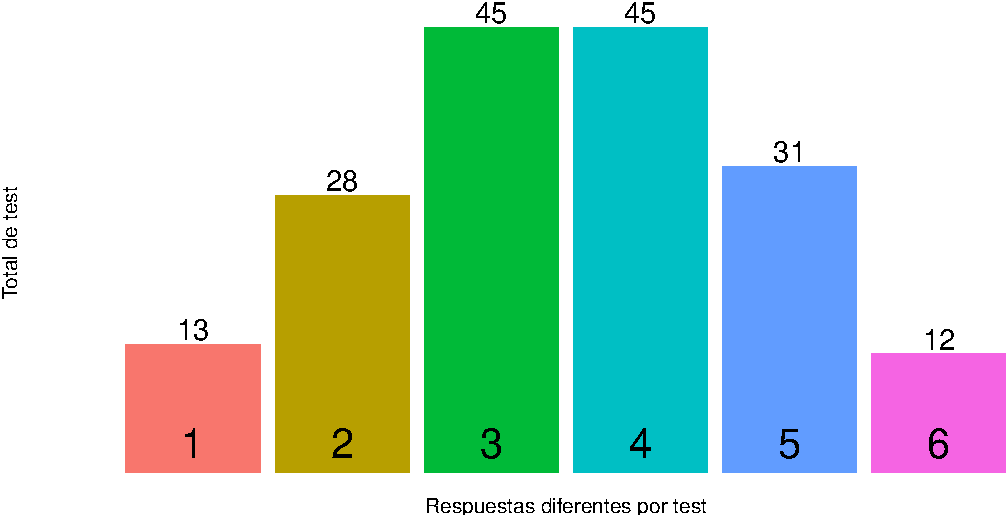
\includegraphics{4_files/figure-pdf/fig-distinct-1.pdf}

}

\caption{\label{fig-distinct}Número de respuestas diferentes en un mismo
test.}

\end{figure}

La tabla Tabla~\ref{tbl-distinct2} muestra los test de respuesta única y
el valor de esa respuesta. Se aprecia que la mayoría de estos test
tienen valor de respuesta 4, la secuencia mayoritaria es la \(BA\) y el
test el \(A\). El estudiante 4 responde ambos test utilizando el mismo
valor de respuesta en todos los ítems.

\hypertarget{tbl-distinct2}{}
\begin{longtable}{rllr}
\caption{\label{tbl-distinct2}Test en los que todos los ítems se contestan con el mismo valor de
respuesta. }\tabularnewline

\toprule
Response & Seq & Test & Subject \\ 
\midrule
2 & AB & A & 4 \\ 
2 & AB & B & 4 \\ 
3 & BA & B & 734 \\ 
3 & BA & A & 803 \\ 
3 & BA & A & 33 \\ 
3 & BA & A & 229 \\ 
4 & AB & A & 35 \\ 
4 & AB & A & 76 \\ 
4 & AB & B & 523 \\ 
4 & BA & B & 85 \\ 
4 & BA & A & 901 \\ 
4 & BA & A & 808 \\ 
4 & BA & A & 871 \\ 
\bottomrule
\end{longtable}

La Figura~\ref{fig-compare} presenta la distribución de la cantidad de
respuestas cuyo valor cambia entre los dos test que realiza cada
estudiante. La mayoría de los estudiantes cambian entre uno y otro test
entre 11 y 17 respuestas. Tan solo 1 estudiante respondió a todos los
ítems con el mismo valor en los dos test. Por otro lado, no hay test que
tengan un número excesivo de contestaciones \enquote{No sé/No contesto}
(ver Tabla~\ref{tbl-noanswer}).

\begin{figure}[h]

{\centering 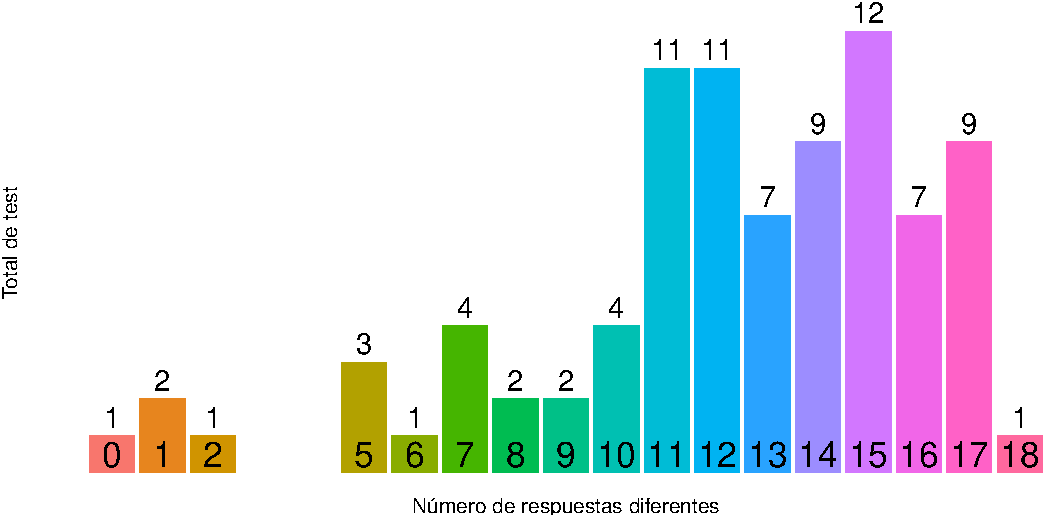
\includegraphics{4_files/figure-pdf/fig-compare-1.pdf}

}

\caption{\label{fig-compare}Número de respuestas diferentes entre los
test para cada estudiante.}

\end{figure}

Tan solo 1 estudiante respondió a todos los ítems con el mismo valor en
los dos test. Por otro lado, no hay test que tengan un número excesivo
de contestaciones \enquote{No sé/No contesto} (ver
Tabla~\ref{tbl-noanswer}).

\hypertarget{tbl-noanswer}{}
\begin{longtable}{lrr}
\caption{\label{tbl-noanswer}Los 5 test con más respuestas `No sé / No contesto' }\tabularnewline

\toprule
Test & Subject & Total answers by test \\ 
\midrule
A & 231 & 5 \\ 
B & 339 & 5 \\ 
B & 346 & 5 \\ 
B & 1174 & 5 \\ 
A & 1187 & 4 \\ 
\bottomrule
\end{longtable}

Se constata que algunos test tienen valores que no parecen muy
razonables. Por ejemplo, no parece razonable realizar la actividad en
menos de 120 segundos. Se observa que en algunos test hay poca
variabilidad. Sin embargo, no son muchos los test con estas
características así que se ha decidido mantener estos datos a pesar de
que se pueda dudar de si en ellos los estudiantes contestaron con la
debida atención y diligencia.

\hypertarget{sec-eda-3}{%
\subsection{\texorpdfstring{Comparación de los subtítulos \(A\) y \(B\)
entre
grupos}{Comparación de los subtítulos A y B entre grupos}}\label{sec-eda-3}}

La Figura~\ref{fig-diff} presenta una forma de comparar los dos test
realizados por los estudiantes. Para cada estudiante se comparó ítem a
ítem sus dos test y se contabilizó la diferencia entre el número de
ítems en los que la puntuación en el segundo vídeo fue superior y en los
que lo fue inferior (las que no variaron de puntuación no se
consideraron). En el eje \(x\) se muestran las diferencias entre
respuestas. Cantidades negativas indican que hay más respuestas en el
segundo de los test que han empeorado respecto al primero de las que han
mejorado. En el eje \(y\) se representa el número de estudiantes para
cada diferencia. Esta frecuencia se representa en negativo cuando la
diferencia en el eje x sea negativa para facilitar la
comparación\footnote{En la comparación se han omitido aquellas
  respuestas en las que el estudiante contestó \enquote{No sé / No
  contesto} en el ítem correspondiente de uno de los test.}. Esto es una
forma de evaluar si el estudiante valoró mejor o no el segundo vídeo que
el primero.

\begin{figure}[h]

{\centering 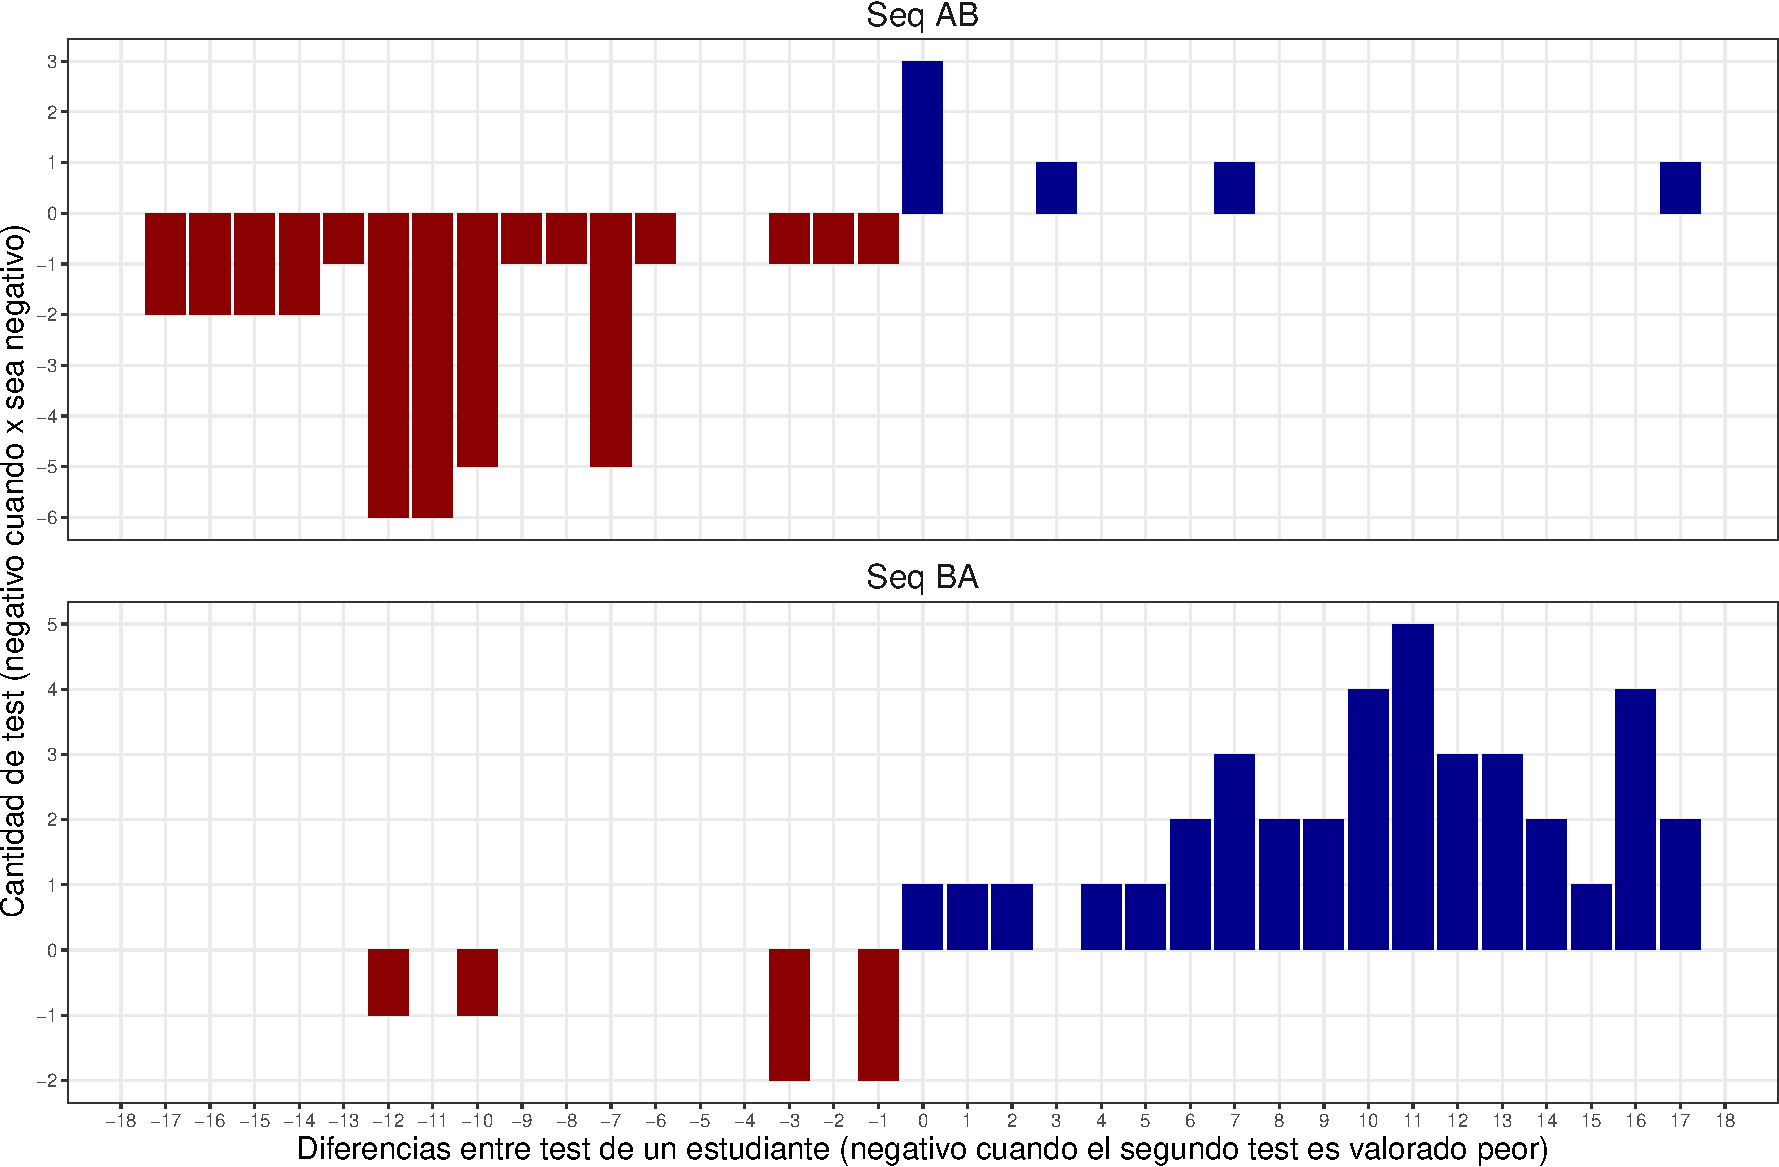
\includegraphics{4_files/figure-pdf/fig-diff-1.pdf}

}

\caption{\label{fig-diff}Diferencias en las respuestas entre test por
estudiante y grupo.}

\end{figure}

Se aprecia que en el grupo \(AB\) las diferencias tienden a ser
negativas y en el \(BA\) positivas. Esto estaría indicando que los
estudiantes valoran mejor el subtitulado de nivel \(A\) en ambas
secuencias. Por ello es esperable que las respuestas de los estudiantes
del grupo \(AB\) hayan empeorado y que las diferencias sean negativas y
que lo contrario haya sucedido con las del grupo \(BA\). La diferencia
más frecuente en el grupo \(AB\) es 12 y en el grupo \(BA\) este valor
es 11. Resulta llamativo que haya estudiantes cuyas contestaciones estén
tan alejadas de la tendencia de su grupo. En la Tabla~\ref{tbl-diff} se
muestran los tiempos que han transcurrido entre la realización de los
test de aquellos estudiantes cuyas respuestas difieren de forma
importante de su grupo. Son aquellos que aparecen en azul en la
secuencia \(AB\) y en rojo en la secuencia \(BA\). Se observa que casi
todos son tiempos entre actividades muy cortos. En cualquier caso y,
como no son muchos, se ha decidido no eliminarlos y realizar el análisis
con ellos.

\hypertarget{tbl-diff}{}
\begin{longtable}{lrrc}
\caption{\label{tbl-diff}Estudiantes que tienen diferencias en sus respuestas muy alejadas de la
tendencia de su grupo. }\tabularnewline

\toprule
Seq & Subject & Diff & Minutes \\ 
\midrule
AB & 1020 & 17 & 1.3 \\ 
AB & 75 & 7 & 3.33 \\ 
BA & 650 & -10 & 50345.95 \\ 
BA & 85 & -12 & 1.7 \\ 
\bottomrule
\end{longtable}

\hypertarget{tbl-resume}{}
\begin{longtable}{cccrrrrrr}
\caption{\label{tbl-resume}Resumen de frecuencias de respuesta. }\tabularnewline

\toprule
 &  &  &  & \multicolumn{5}{c}{Response} \\ 
\cmidrule(lr){5-9}
Seq & Period & Treat & 0 & 1 & 2 & 3 & 4 & 5 \\ 
\midrule
AB & 1 & A & 39 & 2 & 25 & 71 & 203 & 434 \\ 
AB & 2 & B & 43 & 87 & 185 & 121 & 172 & 166 \\ 
BA & 1 & B & 40 & 76 & 174 & 127 & 237 & 138 \\ 
BA & 2 & A & 30 & 2 & 30 & 64 & 345 & 321 \\ 
\bottomrule
\end{longtable}

En la Tabla~\ref{tbl-resume} se muestra la frecuencia absoluta del valor
de respuesta para cada grupo y test en todos los ítems. Esta es otra
forma de comparar los niveles de subtitulado. La Figura~\ref{fig-freqs}
muestra la misma información gráficamente y con frecuencias relativas.
En esta figura se pueden apreciar algunas cuestiones interesantes:

\begin{itemize}
\item
  El tratamiento (subtitulado) con nivel \(A\) presenta claramente
  mayores valores de respuesta que el \(B\) como ya se había visto (ver
  Figura~\ref{fig-diff}).
\item
  En general los dos grupos muestran bastante acuerdo en el subtitulado
  en ambos niveles: En el nivel de tratamiento \(A\) los dos grupos
  tienen una frecuencia relativa similar de respuestas positivas
  (valores 4 y 5). El grupo \(AB\) tiene un 82\% de respuestas positivas
  y el grupo \(BA\) 84\%. No obstante, el grupo \(AB\) tiene más
  respuestas con valor 5 que el grupo \(BA\) (56\% frente a 41\%). La
  valoración es también similar entre grupos en el nivel de tratamiento
  \(B\): el grupo \(AB\) tiene 44\% de respuestas positivas y 47\% el
  grupo \(BA\). Las valoraciones negativas (1, 2), la neutra (3) y la
  \enquote*{No sé / No contesto} (0) son también muy similares en ambos
  grupos.
\end{itemize}

\begin{figure}[h]

{\centering 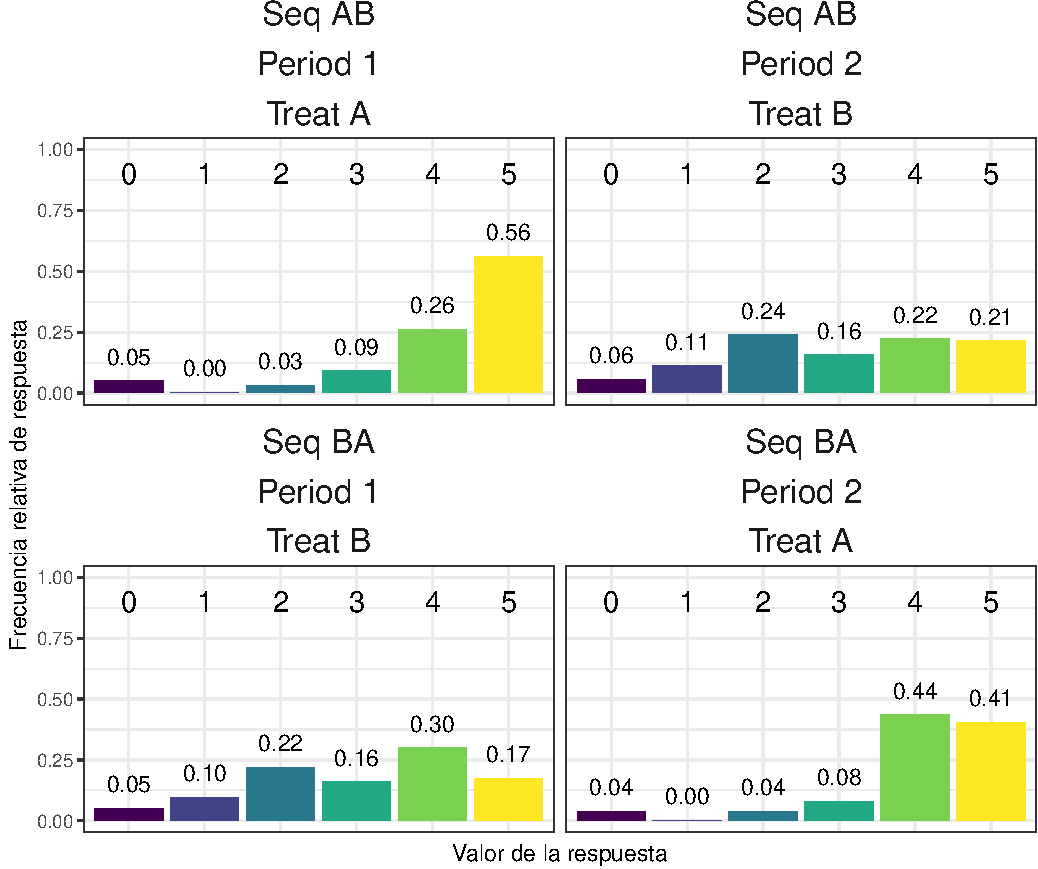
\includegraphics{4_files/figure-pdf/fig-freqs-1.pdf}

}

\caption{\label{fig-freqs}Frecuencias relativas de las respuestas al
test.}

\end{figure}

El análisis marginalizado de tratamiento, secuencia y periodo tiene
estos resultados referidos a los ítems con contestación positiva (4, 5):

\begin{itemize}
\item
  El tratamiento \(A\) tiene un 83\% marginalizado de respuestas
  positivas frente al 46\% del tratamiento \(B\).
\item
  El periodo 1 tiene un 65\% marginalizado de respuestas positivas
  frente al 64\% del periodo 2.
\item
  Finalmente, la secuencia \(AB\) tiene un 63\% de respuestas positivas
  frente 66\% de la secuencia \(BA\).
\end{itemize}

\hypertarget{anuxe1lisis-de-los-uxedtems}{%
\subsection{Análisis de los ítems}\label{anuxe1lisis-de-los-uxedtems}}

El gráfico Figura~\ref{fig-levels} muestra la frecuencia relativa por
grupo y por test de los ítems clasificados por niveles de respuesta,
considerando que:

\begin{itemize}
\tightlist
\item
  Los niveles 1 y 2 se consideran valoraciones negativas.
\item
  El nivel 3 se considera neutro.
\item
  Los niveles 4 y 5 se consideran positivos.
\item
  El nivel 0 (\enquote{No sé / No contesto}) se excluye en este
  análisis.
\end{itemize}

Se muestra en primer lugar el ítem 18 por ser una valoración global del
subtitulado y que resume la opinión que sobre el mismo tiene el
estudiante. Se vuelve a constatar que el subtitulado \(A\) es mejor
valorado por los estudiantes, pero ahora se confirma que en los 18 ítems
ambos grupos tienen más puntuaciones positivas y menos negativas en el
subtitulado \(A\) que en el \(B\). También se vuelve a constatar que los
dos grupos valoran de forma muy similar los dos niveles de subtitulado
en todos los ítems. En el nivel de subtitulado \(A\) los ítems \(Q15\),
\(Q16\) y \(Q17\) obtienen relativamente peores valoraciones (consultar
la Tabla~\ref{tbl-likert-scale} para ver el texto de los ítems) y estas
son similares en ambos subtitulados. Hay algunos ítems que son valoradas
de forma positiva incluso en el nivel de subtitulado \(B\) (por ejemplo
\(Q04\) o \(Q13\)). Por último, los ítems \(Q05\) y \(Q09\) (también la
\(Q14\) pero solo para el grupo \(BA\)) tienen una valoración muy
negativa en el nivel de subtitulado \(B\).

\begin{figure}[h]

{\centering 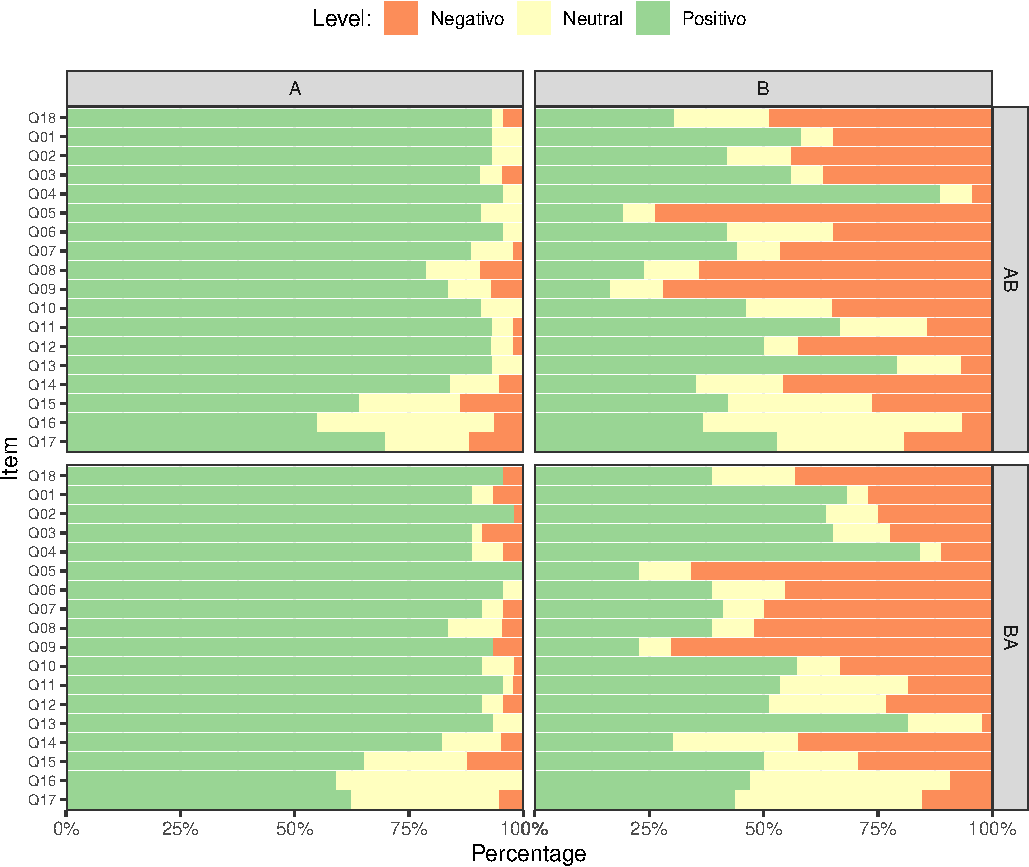
\includegraphics{4_files/figure-pdf/fig-levels-1.pdf}

}

\caption{\label{fig-levels}Frecuencias relativas de las respuestas por
ítem.}

\end{figure}

En la Tabla~\ref{tbl-no-response} se muestran las contestaciones
\enquote{No sé / No contesto} por subtitulado e ítem. Se observa que hay
relativamente pocas contestaciones \enquote{No śe / No contesto} y que
éstas se concentran en los ítems \(Q14\), \(Q15\), \(Q16\) y \(Q17\).

\tiny

\hypertarget{tbl-no-response}{}
\begin{longtable}{rrrrrrrrrrrrrrrrrr}
\caption{\label{tbl-no-response}Contestaciones ``No sé / No contesto'' por nivel de subtitulado e ítem }\tabularnewline

\toprule
Q18 & Q01 & Q02 & Q03 & Q04 & Q05 & Q06 & Q07 & Q08 & Q09 & Q10 & Q11 & Q12 & Q13 & Q14 & Q15 & Q16 & Q17 \\ 
\midrule
\multicolumn{18}{l}{A} \\ 
\midrule
0 & 0 & 0 & 1 & 0 & 0 & 1 & 0 & 3 & 1 & 0 & 1 & 1 & 0 & 11 & 11 & 22 & 17 \\ 
\midrule
\multicolumn{18}{l}{B} \\ 
0 & 0 & 0 & 4 & 0 & 1 & 0 & 0 & 1 & 0 & 8 & 2 & 4 & 1 & 10 & 15 & 25 & 12 \\ 
\bottomrule
\end{longtable}

\normalsize

\hypertarget{sec-modelos-utilizados}{%
\section{Modelos utilizados}\label{sec-modelos-utilizados}}

Es esta sección concreta la forma de aplicar los modelos presentados en
el Marco teórico (ver Capítulo~\ref{sec-arte}) en la actividad de
subtitulado.

\hypertarget{sec-or-2}{%
\subsection[Comparación con \emph{Odds Ratio}
]{\texorpdfstring{Comparación con \emph{Odds Ratio}
\footnote{Esta técnica se ha omitido en el Marco teórico por
  considerarla conocida por el lector. Si se desea ampliar información
  se puede consultar \textcite[p.~18]{agresti2010}.}}{Comparación con Odds Ratio }}\label{sec-or-2}}

La métrica \emph{\gls{odds ratio}} (\(OR\)) permite medir la asociación
entre dos variables con dos niveles cada una. En el diseño de
experimento que se está analizando, los factores \(Treat\), \(Period\) y
\(Seq\) tienen todos 2 niveles y se puede contrastar si hay interacción
entre cada par de factores para cada nivel de respuesta. Es decir, se
contrasta la hipótesis \(H_0: OR=1\) de ausencia de interacción frente a
\(H_1: OR \neq 1\) de existencia de interacción en algún nivel de
respuesta. Por ejemplo, el \(OR\) para el nivel respuesta \(r\) entre
subtítulos y secuencias se define de la siguiente forma:

\[
OR_{(Treat, Seq \mid Response=r)}=\frac{
    \frac{
            P(Treat=A \mid Seq=AB, Response=r)
        }{
            P(Treat=B \mid Seq=AB, Response=r)
        }
    }
    {\frac{
        P(Treat=A \mid Seq=BA, Response=r)
        }{
        P(Treat=B \mid Seq=BA, Response=r)
    }
}
\]

Si los \(\gls{odds}\) son similares en cada nivel de respuesta, se
acepta la hipótesis nula de que los grupos responden de forma similar a
cada nivel de subtitulado. En la Sección~\ref{sec-or-3} se puede
consultar los resultados obtenidos. En esta misma sección se hace un
test similar pero entre subtitulado y periodos. Para realizar el
contraste de hipótesis se usa la función \(loddsratio\) del paquete
\texttt{vcd} \autocite[ver][]{vcd}.

\hypertarget{sec-logistica-2}{%
\subsection{Regresión Logística}\label{sec-logistica-2}}

En la Sección~\ref{sec-logistica} se presentó el fundamento teórico de
la \gls{Regresión Logística}. En esta sección se justifica el uso de
este modelo y se ajustan y comparan varios modelos. La variable
respuesta se compone de 5 valores ordenados. Esto imposibilita usar
directamente la Regresión Logística ya que requiere que la variable de
respuesta sea dicotómica. No obstante, se puede comparar la respuesta
que cada estudiante dio a cada uno de los subtitulados y comprobar si ha
mejorado. Esto producirá una variable de respuesta binaria que permitirá
el uso de la Regresión Logística. No obstante, esta transformación
reducirá la cantidad de datos disponibles a la mitad e impedirá analizar
el \gls{efecto periodo} ya que al comparar los subtitulados, desaparece
el periodo. Se ha creado una variable \texttt{Improve} con dos valores
posibles: 1 cuando el estudiante valoró el ítem mejor en el subtitulado
\(A\) que en el \(B\), 0 si empeoró o puntuó igual. Si en uno de los
test contestó un ítem con \enquote{No sé / No contesto}, se elimina ese
ítem.

Se ajusta el modelo con la secuencia como predictor:

\scriptsize

\begin{Shaded}
\begin{Highlighting}[]
\NormalTok{glm\_improve\_seq }\OtherTok{\textless{}{-}} \FunctionTok{glm}\NormalTok{(Improve }\SpecialCharTok{\textasciitilde{}} \DecValTok{1} \SpecialCharTok{+}\NormalTok{ Seq, }\AttributeTok{family =} \StringTok{"binomial"}\NormalTok{, }\AttributeTok{data =}\NormalTok{ df\_improve)}
\FunctionTok{summary}\NormalTok{(glm\_improve\_seq)}
\end{Highlighting}
\end{Shaded}

\begin{verbatim}

Call:
glm(formula = Improve ~ 1 + Seq, family = "binomial", data = df_improve)

Coefficients:
            Estimate Std. Error z value Pr(>|z|)    
(Intercept)  0.36572    0.08563   4.271 1.94e-05 ***
SeqBA       -0.18153    0.11913  -1.524    0.128    
---
Signif. codes:  0 '***' 0.001 '**' 0.01 '*' 0.05 '.' 0.1 ' ' 1

(Dispersion parameter for binomial family taken to be 1)

    Null deviance: 1575.8  on 1151  degrees of freedom
Residual deviance: 1573.5  on 1150  degrees of freedom
AIC: 1577.5

Number of Fisher Scoring iterations: 4
\end{verbatim}

\normalsize

Se constata que el coeficiente del intercepto es positivo y
significativo (0.37). El intercepto es el \(log\ odds\) de mejorar la
valoración en \(A\) sobre \(B\) respecto a empeorar la valoración. La
probabilidad de que la respuesta a un ítem sea mejor en el subtitulado
\(A\) que en el \(B\) es 0.59. Sin embargo, la secuencia no resulta
significativa y además añadirla apenas reduce la \enquote{deviance}, por
lo que el modelo nulo sin predictores resulta más parsimonioso.

Otra forma de plantear una Regresión Logística es crear una variable de
respuesta dicotómica que tenga valor 1 cuando la respuesta sea positiva
(valores 4 ó 5) y cero cuando no lo sea (valores 1, 2 ó 3). En la
Sección~\ref{sec-ordinal-3} se comentan los resultados de este modelo.

\hypertarget{sec-ordinal-2}{%
\subsection{Regresión Ordinal}\label{sec-ordinal-2}}

En la Sección~\ref{sec-ordinal} se presentó el fundamento teórico de la
Regresión Ordinal Acumulativa (\(CM\)). En esta sección se comprueban
las hipótesis de este modelo para el experimento del subtitulado de
vídeos y se ajustan varios modelos que tratan de predecir el nivel de
respuesta (variable \texttt{Response}) obtenido en cada uno de los ítems
de Likert. Concretamente, se compara el modelo que tenga como único
predictor el nivel de subtitulado (\texttt{Treat}) con el modelo nulo
(sin predictores) y también con el modelo en el que se han añadido los
predictores \texttt{Period} y \texttt{Seq} para comprobar si hay
significación estadística de la presencia de efectos periodo y secuencia
respectivamente.

\hypertarget{comprobaciuxf3n-de-las-hipuxf3tesis-del-modelo-cm}{%
\subsubsection{\texorpdfstring{Comprobación de las hipótesis del modelo
\(CM\)}{Comprobación de las hipótesis del modelo CM}}\label{comprobaciuxf3n-de-las-hipuxf3tesis-del-modelo-cm}}

El modelo \(CM\) presupone que los \(odds\) entre dos niveles de
respuesta son proporcionales para los mismos valores de variables
explicativas. Como se vio en la Ecuación~\ref{eq-ordinal2}, es
equivalente comprobar que los \(odds\) son proporcionales que comprobar
que la diferencia en \texttt{logits} es constante.

No existe un acuerdo generalmente aceptado sobre como comprobar la
proporcionalidad de \(odds\). Así, por ejemplo, el paquete
\texttt{ordinal} \autocite[ver][]{ordinalR} dispone de la función
\texttt{nominal\_test()} que lo que hace es realizar un test de razón de
verosimilitud para cada predictor ajustando un modelo en el que se ha
relajado la condición de proporcionalidad. Otra posibilidad es utilizar
el Test de Brant \autocite[ver][]{brant1990} que compara los
coeficientes obtenidos con los que resultarían de ajustar cada nivel de
respuesta mediante una Regresión Logística. Finalmente \textcite[ver
pp.~315-316]{harrell2015} propone un método gráfico para verificar la
hipótesis de proporcionalidad de \(odds\). En este trabajo se ha
preferido esta última técnica. Para ello se calcula la diferencia en
\texttt{logits} acumulados entre dos niveles de respuesta consecutivos
en cada valor de cada variable predictiva y se comprueba si las
diferencias son similares. En la Figura~\ref{fig-po.check} se han
calculado para los predictores \texttt{Treat}, \texttt{Period},
\texttt{Seq} y \texttt{Item} las diferencias de \texttt{logits} entre
cada dos niveles consecutivos de respuesta. Se constata que las
diferencias son pequeñas particularmente para el periodo y para la
secuencia. También son moderadas para la mayoría de los ítems. La
diferencia es mayor en el subtitulado en la comparación de los niveles
de respuesta 1 y 2. Con esta evidencia, se acepta la hipótesis de
proporcionalidad de \(odds\). En la Tabla~\ref{tbl-po.check} se muestra
cómo se realiza el cálculo de la diferencia de \(odds\) para el
predictor \texttt{Seq} y así facilitar la comprensión de la construcción
de la figura. En caso de que la proporcinalidad de \(odds\) no se cumpla
existen varias posibilidades. Una sería desechar el modelo ordinal y
usar una Regresión Multinomial. Otra sería relajar la hipótesis de
proporcionalidad de \(odds\) estimando un coeficiente distinto para cada
nivel de respuesta y nivel de factor. La función \texttt{vglm} del
paquete \texttt{VGAM} \autocite[ver][]{VGAMR} permite hacer esto.

\begin{figure}[h]

{\centering 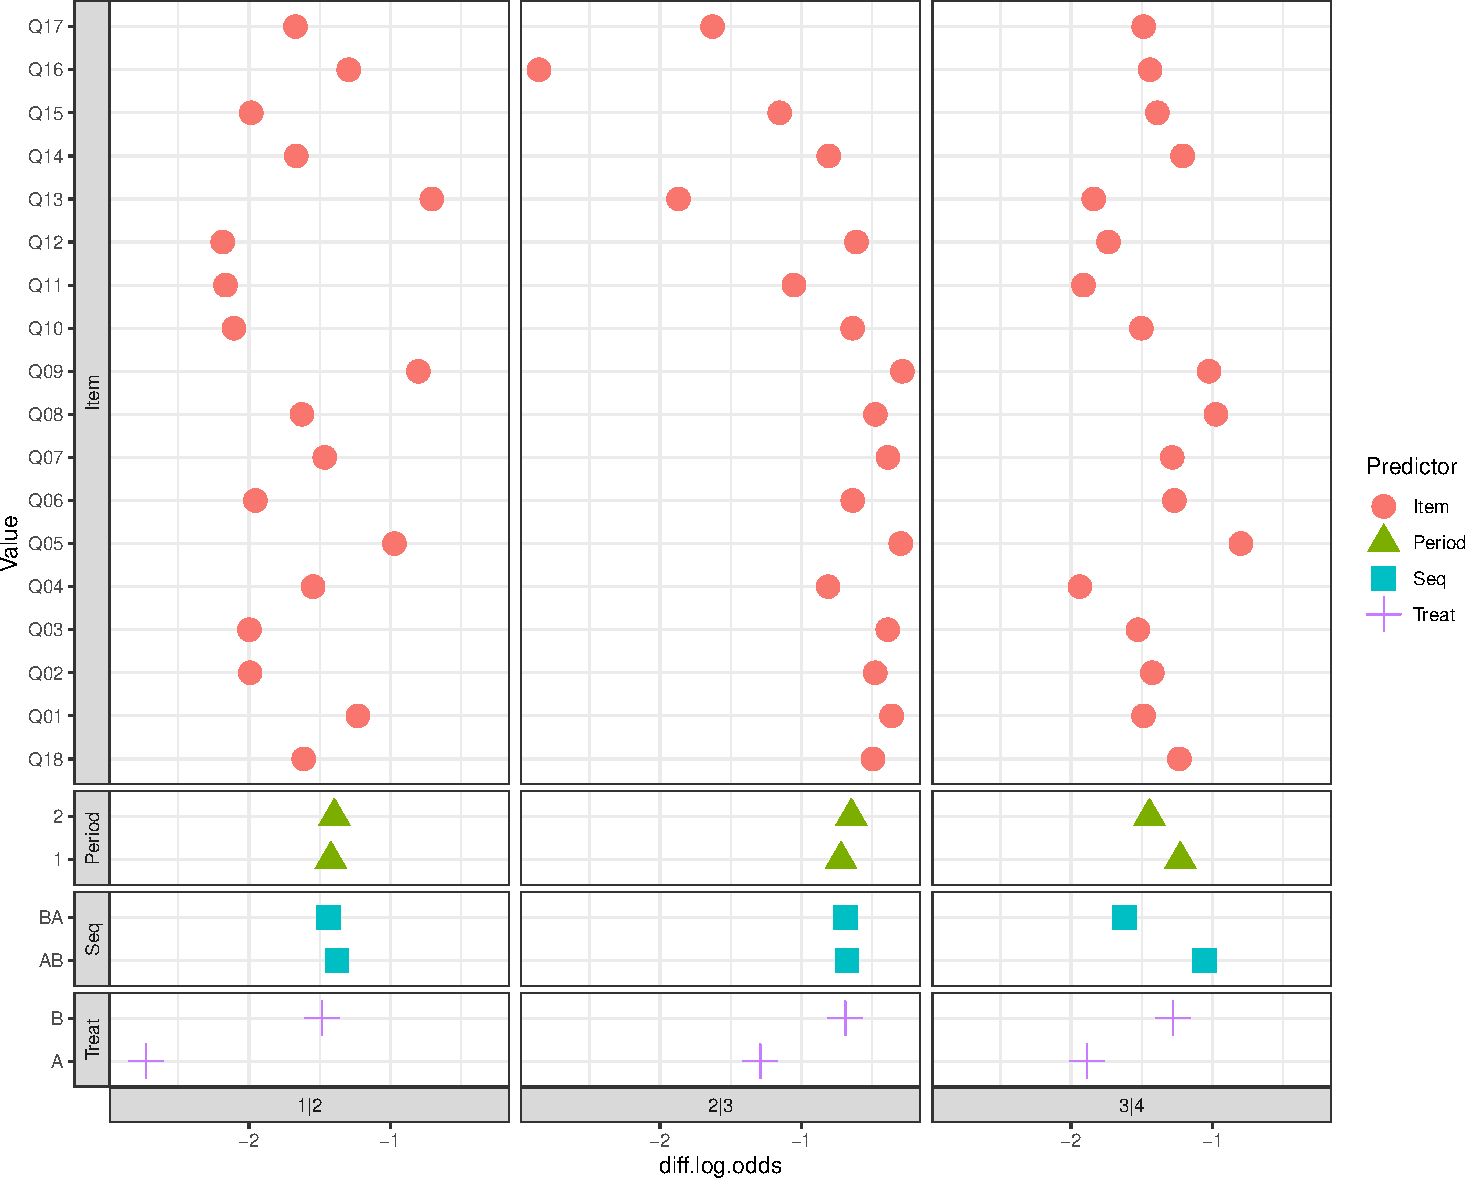
\includegraphics{4_files/figure-pdf/fig-po.check-1.pdf}

}

\caption{\label{fig-po.check}Comprobación de la proporcionalidad de
\emph{odds}.}

\end{figure}

\hypertarget{tbl-po.check}{}
\begin{longtable}{crrrrr}
\caption{\label{tbl-po.check}Comprobación de la proporcionalidad de \emph{odds} para Seq. }\tabularnewline

\toprule
Response & n & cum.sum & odds & log.odds & diff.log.odds \\ 
\midrule
\multicolumn{6}{l}{AB} \\ 
\midrule
1 & 89 & 89 & $0.06$ & $-2.74$ & $-1.38$ \\ 
2 & 210 & 299 & $0.26$ & $-1.36$ & $-0.68$ \\ 
3 & 192 & 491 & $0.50$ & $-0.69$ & $-1.05$ \\ 
4 & 375 & 866 & $1.44$ & $0.37$ & $-Inf$ \\ 
5 & 600 & 1466 & $Inf$ & $Inf$ & NA \\ 
\midrule
\multicolumn{6}{l}{BA} \\ 
\midrule
1 & 78 & 78 & $0.05$ & $-2.91$ & $-1.44$ \\ 
2 & 204 & 282 & $0.23$ & $-1.47$ & $-0.69$ \\ 
3 & 191 & 473 & $0.45$ & $-0.79$ & $-1.62$ \\ 
4 & 582 & 1055 & $2.30$ & $0.83$ & $-Inf$ \\ 
5 & 459 & 1514 & $Inf$ & $Inf$ & NA \\ 
\bottomrule
\end{longtable}

\hypertarget{ajuste-del-modelo-ordinal-response-treat}{%
\subsubsection{\texorpdfstring{Ajuste del modelo ordinal
\texttt{Response\ \textasciitilde{}\ Treat}}{Ajuste del modelo ordinal Response \textasciitilde{} Treat}}\label{ajuste-del-modelo-ordinal-response-treat}}

Existen varios paquetes en R que permiten ajustar un modelo \(CM\) con
función de enlace logística. El más popular es el paquete
\texttt{ordinal} \autocite[ver][]{ordinalR}. El paquete \texttt{VGAM}
\autocite[ver][]{VGAMR} es más flexible y potente. Otra posibilidad es
usar la función \texttt{polr} del paquete \texttt{MASS}
\autocite[ver][]{MASSR}. Finalmente la función \texttt{orm} del paquete
\texttt{rms} también permite hacerlo \autocite[ver][]{harrell2015}. En
este trabajo se usa el paquete \texttt{ordinal}
\autocite[ver][]{ordinalR} por permitir también incluir efectos
aleatorios que se utilizarán en el modelado multinivel. Se comienza con
un modelo simple que tiene como único predictor el nivel de subtitulado
por ser la variable más importante al ser el objeto de la pregunta de
investigación:

\[
\text{logit}(P(Response_i \leq k)) = \tau_k - \beta_1 \text{Treat}_i,
\]

\scriptsize

\begin{Shaded}
\begin{Highlighting}[]
\NormalTok{clm\_treat }\OtherTok{\textless{}{-}}
    \FunctionTok{clm}\NormalTok{(}
\NormalTok{        Response }\SpecialCharTok{\textasciitilde{}}\NormalTok{ Treat,}
        \AttributeTok{data =}\NormalTok{ df\_response, }\AttributeTok{link =} \StringTok{"logit"}
\NormalTok{    )}
\FunctionTok{summary}\NormalTok{(clm\_treat)}
\end{Highlighting}
\end{Shaded}

\begin{verbatim}
formula: Response ~ Treat
data:    df_response

 link  threshold nobs logLik   AIC     niter max.grad cond.H 
 logit flexible  2980 -3966.11 7942.21 5(0)  1.64e-10 3.1e+01

Coefficients:
       Estimate Std. Error z value Pr(>|z|)    
TreatB  -1.7206     0.0731  -23.54   <2e-16 ***
---
Signif. codes:  0 '***' 0.001 '**' 0.01 '*' 0.05 '.' 0.1 ' ' 1

Threshold coefficients:
    Estimate Std. Error z value
1|2 -3.97230    0.09678 -41.045
2|3 -2.45446    0.06812 -36.029
3|4 -1.66453    0.05936 -28.042
4|5 -0.10547    0.04946  -2.132
\end{verbatim}

\normalsize

La función \texttt{summary()} muestra la información resumen. Para su
interpretación se va a seguir \textcite{christensen2018CumulativeLM}. El
número de condición Hessiano es inferior a \(10^4\) lo que es indicativo
de que no hay problemas de optimización \footnote{El número de condición
  de Hessiano es una medida de la curvatura de una función en un punto.
  Si el número de condición de Hessiano es grande, la función es muy
  sensible a pequeñas perturbaciones y puede ser difícil de optimizar.}.
La sección de coeficientes es la más importante. Se muestra la
estimación de parámetros, el error estándar y la significación
estadística de acuerdo al test de Wald \footnote{El test de Wald es un
  contraste de hipótesis estadístico en el que se evalúa si el valor
  estimado es cero suponiendo que
  \(W = \left(\frac{\hat{\theta} - \theta_0}{se(\hat{\theta})}\right)^2 \sim \chi^{2}\)
  .}. Se comprueba que el valor es claramente significativo. Es decir,
que los estudiantes han valorado de forma diferente la calidad del
subtitulado en ambos vídeos. El estimador de maxima verosimilitud del
coeficiente \texttt{TreatB} es -1.72. Siguiendo la deducción de
\textcite{bruin2011} se puede, por ejemplo, hacer la siguiente
interpretación del significado de este coeficiente referido a dos
niveles consecutivos de respuesta, por ejemplo 1 y 2:

\[
\begin{aligned}
logit [P(Y \le 1)] & = & -3.97 - (-1.72 x_1) \\
logit [P(Y \le 2)] & = & -2.45 - (-1.72 x_1)
\end{aligned}
\]

Por lo tanto y teniendo en cuenta que \(x_1 = 1\) cuando \(Treat = B\) y
\(x_1 = 0\) cuando \(Treat = A\), se pueden calcular los \(odds\) de
\(A\) y de \(B\):

\[
\begin{aligned}
\frac{P(Y \le 1 \mid x_1 = B)}{P(Y > 1 \mid x_1 = B)} & = & exp(-3.97)/exp(-1.72) \\
\frac{P(Y \le 1 \mid x_1 = A)}{P(Y > 1 \mid x_1 = A)} & = & exp(-3.97) \\
\frac{P(Y \le 2 \mid x_1 = B)}{P(Y > 2 \mid x_1 = B)} & = & exp(-2.45)/exp(-1.72) \\
\frac{P(Y \le 2 \mid x_1 = A)}{P(Y > 2 \mid x_1 = A)} & = & exp(-2.45)
\end{aligned}
\]

Y los \(OR\) del subtitulado \(B\) sobre \(A\) para los niveles de
respuesta 1 y 2:

\[
\begin{aligned}
\frac{P(Y \le 1 | x_1=B)}{P(Y > 1 | x_1=B)} / \frac{P(Y \le 1 | x_1=A)}{P(Y > 1 | x_1=A)} & = & 1/exp(-1.72) & = & 5.59 \\
\frac{P(Y \le 2 | x_1=B)}{P(Y > 2 | x_1=B)} / \frac{P(Y \le 2 | x_1=A)}{P(Y > 2 | x_1=A)} & = & 1/exp(-1.72) & = & 5.59 \\
\end{aligned}
\]

Se comprueba que el \(OR\) es equivalente en todos los niveles de
respuesta al cuestionario. Esta es una la suposición principal de los
modelos \(CM\). El \(odds\) de respuesta al cuestionario entre los
niveles inferiores y superiores a uno dado, \(k\), es 5.59 veces en el
subtitulado \(B\) que en el \(A\). Esto indica que el subtitulado \(B\)
es percibido por los estudiantes como de peor calidad que el subtitulado
\(A\). Concretamente, el \texttt{OR} de observar una mejor respuesta en
un ítem del test es 5.59 veces superior en el nivel de subtitulado \(A\)
que en el \(B\). Aunque no suele ser de interés la interpretación de los
coeficientes de los umbrales (\texttt{Threshold\ coefficients}), se
pueden utilizar para estimar las probabilidades de respuesta. Por
ejemplo, para el nivel de subtitulado \(B\) y nivel de respuesta 2:

\[
\begin{aligned}
logit [P(Y \le 1)] & = & -3.97 - (-1.72) & = & -2.25 \\
P(Y \le 1) & = & \frac{exp(-2.25)}{1 + exp(-2.25)} & = & 0.10 \\
logit [P(Y \le 2)] & = & -2.45 - (-1.72) & = & -0.73 \\
P(Y \le 2) & = & \frac{exp(-0.73)}{1 + exp(-0.73)} & = & 0.32 \\
P(Y = 2) & = & P(Y \le 2) - P(Y \le 1) & = &  0.23 
\end{aligned}
\]

Para el subtitulado \(A\) no se tiene en cuenta el coeficiente
\(TreatB\) ya que el valor \(x_1\) es cero:

\[
\begin{aligned}
logit [P(Y \le 1)] & = & & & -3.97 \\
P(Y \le 1) & = & \frac{exp(-3.97)}{1 + exp(-3.97)} & = & 0.02 \\
logit [P(Y \le 2)] & = & & & -2.45 \\
P(Y \le 2) & = & \frac{exp(-2.45)}{1 + exp(-2.45)} & = & 0.08 \\
P(Y = 2) & = & P(Y \le 2) - P(Y \le 1) & = &  0.06 
\end{aligned}
\]

En Tabla~\ref{tbl-probs-clm-treat} se muestran las probabilidades para
ambos niveles de subtitulado y todos los posibles valores de respuesta.
Se confirma que en el nivel de subtitulado \(A\) son más probables las
respuestas 5 y 4, siendo poco probables el resto de niveles. Sin
embargo, en el subtitulado \(B\) existe bastante incertidumbre, siendo
el valor más probable el nivel 4 y muy similares los niveles 2, 3 y 5.
Esto se corresponde con lo que ya se había constatado en el Análisis
Exploratorio (ver Figura~\ref{fig-freqs}). Se debe tener en cuenta que
este modelo tiene un único predictor y, por lo tanto, no es capaz de
explicar las diferencias en el nivel de respuesta para distintos
periodos, secuencias, ítems o estudiantes. En las siguientes secciones
se investiga si en el nivel de respuesta influyen estos predictores.

\hypertarget{tbl-probs-clm-treat}{}
\begin{table}
\caption{\label{tbl-probs-clm-treat}Probabilidades de respuesta para el modelo ordinal Response
\textasciitilde{} Treat }\tabularnewline

\centering
\begin{tabular}{l|r|r|r|r|r}
\hline
  & 1 & 2 & 3 & 4 & 5\\
\hline
A & 0.018 & 0.061 & 0.08 & 0.315 & 0.526\\
\hline
B & 0.095 & 0.229 & 0.19 & 0.320 & 0.166\\
\hline
\end{tabular}
\end{table}

\hypertarget{sec-response-treat.period}{%
\subsubsection{\texorpdfstring{Ajuste del modelo ordinal
\texttt{Response\ \textasciitilde{}\ Treat\ *\ Period}}{Ajuste del modelo ordinal Response \textasciitilde{} Treat * Period}}\label{sec-response-treat.period}}

Para saber si existe un efecto periodo, se añade como predictor la
variable \texttt{Period}. También se añade la interacción entre
subtitulado y periodo \footnote{Se debe tener en cuenta que en R la
  interacción entre dos variables se puede añadir con los símbolos
  \enquote{\(*\)} y \enquote{\(:\)}. El símbolo \enquote{\(*\)} añade al
  modelo tanto los efectos principales como la interacción, mientras que
  el símbolo \enquote{\(:\)} tan solo añade la interacción. Por ello,
  los modelos \(Response \sim Treat*Period\) y
  \(Response \sim Treat + Period + Treat:Period\) son equivalentes en R}:

\small

\begin{equation}\protect\hypertarget{eq-ordinal-3}{}{
\text{logit}(P(Response_i \leq k)) = \tau_k - \beta_1 \text{Treat}_i - \beta_2 \text{Period}_i - \beta_3 \text{Treat}_i : \text{Period}_i
}\label{eq-ordinal-3}\end{equation}

\normalsize

En el Apéndice~\ref{sec-contrasts} se demuestra que cuando el contraste
es \(sum\) la interacción entre periodo y subtitulado es equivalente al
\gls{efecto secuencia}. Es decir, que los modelos
\texttt{Response\ \textasciitilde{}\ Treat*Period} y
\texttt{Response\ \textasciitilde{}\ Treat\ +\ Period\ +\ Seq} son
equivalentes. Esto no sucede cuando el contraste es \(treatment\), que
es el utilizado por defecto en R. En la Tabla~\ref{tbl-contrast} se
comparan los coeficientes de los cuatro modelos que se listan a
continuación:

\begin{itemize}
\tightlist
\item
  \texttt{Response\ \textasciitilde{}\ Treat\ *\ Period} con contraste
  \texttt{treatment}.
\item
  \texttt{Response\ \textasciitilde{}\ Treat\ +\ Period\ +\ Seq} con
  contraste \texttt{treatment}.
\item
  \texttt{Response\ \textasciitilde{}\ Treat\ *\ Period} con contraste
  \texttt{sum}.
\item
  \texttt{Response\ \textasciitilde{}\ Treat\ +\ Period\ +\ Seq} con
  contraste \texttt{sum}.
\end{itemize}

\tiny

\hypertarget{tbl-contrast}{}
\begin{longtable}{lrlrlrlr}
\caption{\label{tbl-contrast}Comparación de los coeficientes con contraste ``treatment'' y ``sum''. }\tabularnewline

\toprule
\multicolumn{4}{c}{contr.treatment} & \multicolumn{4}{c}{contr.sum} \\ 
\cmidrule(lr){1-4} \cmidrule(lr){5-8}
\multicolumn{2}{c}{Response \textasciitilde{} Treat*Period} & \multicolumn{2}{c}{Response \textasciitilde{} Treat+Period+Seq} & \multicolumn{2}{c}{Response \textasciitilde{} Treat*Period} & \multicolumn{2}{c}{Response \textasciitilde{} Treat+Period+Seq} \\ 
\cmidrule(lr){1-2} \cmidrule(lr){3-4} \cmidrule(lr){5-6} \cmidrule(lr){7-8}
coef & value & coef & value & coef & value & coef & value \\ 
\midrule
1|2 & $-4.246$ & 1|2 & $-4.246$ & 1|2 & $-3.127$ & 1|2 & $-3.127$ \\ 
2|3 & $-2.728$ & 2|3 & $-2.728$ & 2|3 & $-1.608$ & 2|3 & $-1.608$ \\ 
3|4 & $-1.938$ & 3|4 & $-1.938$ & 3|4 & $-0.818$ & 3|4 & $-0.818$ \\ 
4|5 & $-0.370$ & 4|5 & $-0.370$ & 4|5 & $0.750$ & 4|5 & $0.750$ \\ 
TreatB & $-1.960$ & TreatB & $-1.748$ & Treat1 & $0.874$ & Treat1 & $0.874$ \\ 
Period2 & $-0.492$ & Period2 & $-0.279$ & Period1 & $0.140$ & Period1 & $0.140$ \\ 
TreatB:Period2 & $0.425$ & SeqBA & $-0.213$ & Treat1:Period1 & $0.106$ & Seq1 & $0.106$ \\ 
\bottomrule
\end{longtable}

\normalsize

Se comprueba que coinciden los coeficientes de los dos modelos con
contraste \texttt{sum} y que el efecto secuencia es equivalente a la
interacción de periodo y subtitulado con este contraste. Sin embargo, en
el contraste \texttt{treatment} coinciden los coeficientes de los
interceptores pero no así los de los factores. Además, estos tres
últimos coeficientes tienen nombres diferentes en los dos contrastes. La
diferencia en el nombre se corresponde con la distinta interpretación
del significado de los coeficientes. En el contraste \texttt{treatment}
los valores de los interceptos se refieren a los valores de los factores
en el nivel de referencia de cada factor (en este caso \(Treat = A\) y
\(Period = 1\)) y los valores de los otros coeficientes (\(TreatB\) y
\(Period2\)) son la diferencia con el de referencia. Así, por ejemplo,
\(TreatB\) es la diferencia con \(TreatA\) en el periodo 1. Con este
tipo de contraste es más difícil aislar el efecto que produce un nivel
de un factor independiente del otro factor. En el contraste \texttt{sum}
los valores de los interceptos son el efecto medio \footnote{Se calcula
  como la media de las medias de cada combinación de los niveles de
  factor.}, y los coeficientes \(Treat1\) y \(Period1\) son los efectos
que sobre ese valor medio produce el nivel de factor de referencia, que
en este caso es el primero (\(Treat = A\) y \(Period = 1\)
respectivamente). Así por ejemplo en el contraste \texttt{sum}:

\begin{itemize}
\tightlist
\item
  El coeficiente \(1|2\) tiene un valor -3.127 y es el \texttt{logit}
  medio de que la respuesta sea menor que 1 frente a que sea mayor que
  1.
\item
  El coeficiente \(Treat1\) tiene un valor de 0.874 y es la diferencia
  en \texttt{logits} que se añade en el nivel de subtitulado \(A\) sin
  tener en cuenta el periodo. Es decir, que es el efecto del subtitulado
  \(A\). Su valor es positivo. Como en la Ecuación~\ref{eq-ordinal-3}
  aparece restando, el subtitulado \(A\) hace más pequeño el
  \texttt{logit} y, por lo tanto, disminuye la probabilidad de una
  respuesta inferior frente a una superior.
\item
  Para obtener el efecto del subtitulado \(B\) se cambia el signo a
  \(Treat1\): -0.874. Por ello aumenta la probabilidad de un menor valor
  de respuesta.
\item
  La diferencia en \texttt{logits} de los efectos totales del
  subtitulado es el doble de 0.874.
\item
  El coeficiente \(Period1\) tiene un valor 0.14 y es la diferencia en
  \texttt{logits} que produce el periodo \(1\) sin tener en cuenta el
  subtitulado.
\item
  El efecto del periodo \(2\) se obtiene cambiado el signo al efecto del
  periodo 1: -0.14.
\item
  El efecto total del periodo es 0.279 \texttt{logits}.
\item
  El coeficiente \(Treat1:Period1\) tiene un valor de 0.106 y es la
  interacción entre el subtitulado \(A\) y el periodo \(1\). Es
  equivalente al efecto en \texttt{logits} de la secuencia \(AB\). El
  efecto de la secuencia \(BA\) será -0.106.
\item
  Por lo tanto el efecto total en \texttt{logits} del subtitulado \(A\)
  en el periodo 1 será
  \(1|2 - Treat1 - Period1 - Treat1:Period1 = -3.127 - 0.874 - 0.14 - 0.106 = -4.246\).
  Obsérvese que este valor corresponde con el parámetro \(1|2\) de los
  modelos con contraste \texttt{treatment}.
\item
  El efecto total en \texttt{logits} del subtitulado \(B\) en el periodo
  1 será
  \(1|2 + Treat1 - Period1 + Treat1:Period1 = -3.127 + 0.874 - 0.14 + 0.106\).
\item
  El efecto total en \texttt{logits} del subtitulado \(A\) en el periodo
  2 será
  \(1|2 - Treat1 + Period1 + Treat1:Period1 = -3.127 - 0.874 + 0.14 + 0.106\).
\item
  El efecto total en \texttt{logits} del subtitulado \(B\) en el periodo
  2 será
  \(1|2 + Treat1 + Period1 - Treat1:Period1 = -3.127 + 0.874 + 0.14 - 0.106\).
\end{itemize}

En la Tabla~\ref{tbl-contrat2} se muestra la equivalencia de los
coeficientes entre los modelos ajustados con cada contraste. La
conclusión que se obtiene de todo esto es que cuando se usan dos o más
factores, la interpretación con contraste \texttt{sum} resulta más
intuitiva y sencilla y será el contraste utilizado en este trabajo.

\small

\hypertarget{tbl-contrat2}{}
\begin{longtable}[]{@{}lll@{}}
\caption{\label{tbl-contrat2}Equivalencia entre los coeficientes
\texttt{contr.treatment} y \texttt{contr.sum} en el modelo Response
\textasciitilde{} Treat*Period.}\tabularnewline
\toprule\noalign{}
contr.treatment & contr.sum & value \\
\midrule\noalign{}
\endfirsthead
\toprule\noalign{}
contr.treatment & contr.sum & value \\
\midrule\noalign{}
\endhead
\bottomrule\noalign{}
\endlastfoot
1\textbar2 & 1\textbar2 - Treat1 - Period1 - Treat1:Period1 & -4.246 \\
2\textbar3 & 2\textbar3 - Treat1 - Period1 - Treat1:Period1 & -2.728 \\
3\textbar4 & 3\textbar4 - Treat1 - Period1 - Treat1:Period1 & -1.938 \\
4\textbar5 & 4\textbar5 - Treat1 - Period1 - Treat1:Period1 & -0.37 \\
TreatB & -2(Treat1 + Treat1:Period1) & -1.96 \\
Period2 & -2(Period1 + Treat1:Period1) & -0.492 \\
TreatB:Period2 & 4(Treat1:Period1) & 0.425 \\
\end{longtable}

\normalsize

A continuación se muestra el resumen del modelo con contraste
\texttt{sum} para constatar que los tres coeficientes son
significativos:

\begin{verbatim}
formula: Response ~ Treat * Period
data:    df_response

 link  threshold nobs logLik   AIC     niter max.grad cond.H 
 logit flexible  2980 -3953.01 7920.03 5(0)  2.13e-10 1.4e+01

Coefficients:
               Estimate Std. Error z value Pr(>|z|)    
Treat1          0.87395    0.03678  23.763  < 2e-16 ***
Period1         0.13962    0.03411   4.094 4.25e-05 ***
Treat1:Period1  0.10627    0.03410   3.117  0.00183 ** 
---
Signif. codes:  0 '***' 0.001 '**' 0.01 '*' 0.05 '.' 0.1 ' ' 1

Threshold coefficients:
    Estimate Std. Error z value
1|2 -3.12665    0.08242  -37.94
2|3 -1.60838    0.04968  -32.38
3|4 -0.81849    0.04225  -19.37
4|5  0.74993    0.04194   17.88
\end{verbatim}

\hypertarget{sec-mejor-modelo-efectos-fijos}{%
\subsubsection{Elección del modelo ordinal mediante el test de razón de
verosimilitud}\label{sec-mejor-modelo-efectos-fijos}}

La Tabla~\ref{tbl-ordinal-com} compara tres modelos ordinales con el
contraste \(sum\):

\begin{itemize}
\tightlist
\item
  Modelo nulo.
\item
  Modelo con predictor \texttt{Treat}.
\item
  Modelo con predictores \texttt{Treat} y \texttt{Period} y su
  interacción (que es equivalente a incluir el predictor \texttt{Seq}).
\end{itemize}

Se constata que los coeficientes estimados en los tres modelos son
significativos y de similar valor.

\miniscule

\hypertarget{tbl-ordinal-com}{}
\begin{longtable}{lcccccccccccc}
\caption{\label{tbl-ordinal-com}Comparación de modelos ordinales. }\tabularnewline

\toprule
 & \multicolumn{4}{c}{Response \textasciitilde{} 1    } & \multicolumn{4}{c}{Response \textasciitilde{} Treat    } & \multicolumn{4}{c}{Response \textasciitilde{} Treat:Period    } \\ 
\cmidrule(lr){2-5} \cmidrule(lr){6-9} \cmidrule(lr){10-13}
  & Est. & S.E. & 2.5 \% & 97.5 \% & Est.  & S.E.  & 2.5 \%  & 97.5 \%  & Est.   & S.E.   & 2.5 \%   & 97.5 \%   \\ 
\midrule
1|2  & -2.824*** & 0.080 & -2.980 & -2.668 & -3.112*** & 0.082 & -3.273 & -2.951 & -3.127*** & 0.082 & -3.288 & -2.965 \\ 
2|3  & -1.418*** & 0.046 & -1.509 & -1.327 & -1.594*** & 0.049 & -1.691 & -1.497 & -1.608*** & 0.050 & -1.706 & -1.511 \\ 
3|4  & -0.738*** & 0.039 & -0.815 & -0.661 & -0.804*** & 0.042 & -0.887 & -0.722 & -0.818*** & 0.042 & -0.901 & -0.736 \\ 
4|5  & 0.596*** & 0.038 & 0.521 & 0.671 & 0.755*** & 0.042 & 0.673 & 0.837 & 0.750*** & 0.042 & 0.668 & 0.832 \\ 
Treat1  &  &  &  &  & 0.860*** & 0.037 & 0.789 & 0.932 & 0.874*** & 0.037 & 0.802 & 0.946 \\ 
Period1  &  &  &  &  &  &  &  &  & 0.140*** & 0.034 & 0.073 & 0.206 \\ 
Treat1 × Period1  &  &  &  &  &  &  &  &  & 0.106** & 0.034 & 0.039 & 0.173 \\ 
Num.Obs. & 2980 &  &  &  & 2980 &  &  &  & 2980 &  &  &  \\ 
AIC & 8541.7 &  &  &  & 7942.2 &  &  &  & 7920.0 &  &  &  \\ 
BIC & 8565.7 &  &  &  & 7972.2 &  &  &  & 7962.0 &  &  &  \\ 
Log.Lik. & -4266.851 &  &  &  & -3966.107 &  &  &  & -3953.013 &  &  &  \\ 
edf & 4 &  &  &  & 5 &  &  &  & 7 &  &  &  \\ 
\bottomrule
\end{longtable}

\normalsize

Al ser los tres modelos anidados se pueden comparar con la prueba de
razón de verosimilitud. Se comprueba que el tercer modelo reduce
significativamente el logaritmo de la función de verosimilitud y, por lo
tanto, debe ser aceptado:

\scriptsize

\begin{verbatim}
Likelihood ratio tests of cumulative link models:
 
                     formula:                  link: threshold:
clm_sum_null         Response ~ 1              logit flexible  
clm_sum_treat        Response ~ Treat          logit flexible  
clm_sum_treat.period Response ~ Treat * Period logit flexible  

                     no.par    AIC  logLik LR.stat df Pr(>Chisq)    
clm_sum_null              4 8541.7 -4266.9                          
clm_sum_treat             5 7942.2 -3966.1 601.490  1  < 2.2e-16 ***
clm_sum_treat.period      7 7920.0 -3953.0  26.186  2  2.059e-06 ***
---
Signif. codes:  0 '***' 0.001 '**' 0.01 '*' 0.05 '.' 0.1 ' ' 1
\end{verbatim}

\normalsize

Este modelo estima coeficientes positivos para \texttt{Treat1},
\texttt{Period1} y \texttt{Treat1:Period1} (equivalente a
\texttt{Seq1}). Estos coeficientes indican que:

\begin{itemize}
\tightlist
\item
  Son más probables mayores niveles de respuesta en el subtitulado \(A\)
  que en el \(B\).
\item
  Son más probables mayores niveles de respuesta en el periodo 1 que en
  el 2.
\item
  Son más probables mayores niveles de respuesta en la secuencia \(AB\)
  que en la secuencia \(BA\).
\item
  No obstante, y a pesar de que el efecto periodo y el efecto secuencia
  son significativos, el efecto del nivel de subtitulado medido en
  \texttt{logits} es ocho veces más importante que estos efectos
  considerados individualmente y cuatro veces considerados de forma
  conjunta.
\end{itemize}

\hypertarget{sec-multinivel-2}{%
\subsection{Regresión Ordinal Multinivel}\label{sec-multinivel-2}}

En la Sección~\ref{sec-multinivel} se expuso el fundamento teórico de
los modelos multinivel. Aquí se justifica su interés aplicado al caso
del subtitulado de vídeos. Hay dos variables susceptibles de ser
incorporadas al modelo como efectos aleatorios. El primer candidato es
el factor \texttt{Subject}. Es evidente que los estudiantes son una
muestra de una población más amplia que estaría constituida por todos
los estudiantes del curso de \gls{accesibilidad}. Pero es que además
cada estudiante responde a cada ítem dos veces y, por lo tanto, sus
observaciones no son independientes. En la Figura~\ref{fig-subjects} se
muestran las respuestas de diez estudiantes a cada subtitulado. Se
observa que las respuestas no son independientes ya que cada estudiante
tiene un preferencia por uno o varios niveles de respuesta en cada test.
Por otro lado, los ítems no son independientes unos de otros ya que
pretenden medir la misma variable subyacente. Además, el interés no es
conocer el valor concreto de sus coeficientes sino su valor en relación
a los coeficientes de los otros ítems. En
\textcite[pp.~14-16]{burkner2021} \textcite[pp.~19-20]{burkner2019} se
puede encontrar un ejemplo con esta parametrización aplicada a una
\gls{escala de likert}.

\hypertarget{modelo-response-treat-period-1-subject}{%
\subsubsection{Modelo Response \textasciitilde{} Treat * Period + (1
\textbar{} Subject)}\label{modelo-response-treat-period-1-subject}}

El primer modelo que se propone es un modelo que mantiene los
predictores \texttt{Treat} y \texttt{Period} y su interacción
(equivalente al \gls{efecto secuencia}) como efectos fijos que fueron
seleccionadas en la sección anterior (ver
Sección~\ref{sec-mejor-modelo-efectos-fijos}) e incorpora los
estudiantes como efectos aleatorios sobre los interceptos:

\small

\[
\begin{aligned}
Nivel\ 1: & \text{logit}(P(Response_{ij} \leq k)) = \tau_{kj} - \beta_1 \text{Treat}_{ij} - \beta_2 \text{Period}_{ij} - \beta_3 \text{Treat}_{ij} * \text{Period}_{ij} \\
Nivel\ 2: & \tau_{kj}  =  \tau_{k} + Subject_{0j}
\end{aligned}
\]

\normalsize

donde \(ij\) es la observación \(i\) del estudiante \(j\). Obsérvese que
ahora los interceptos \(\tau_{kj}\) se descomponen en una parte fija y
común para cada nivel de respuesta \(k\), \(\tau_{k}\) y una parte
variable específica para cada estudiante \(Subject_{0j}\). Para ajustar
el modelo se va a utilizar la función \texttt{clmm} del paquete
\texttt{ordinal} \autocite[ver][]{ordinalR} ya que permite la inclusión
de efectos aleatorios.

\scriptsize

\begin{figure}[h]

{\centering 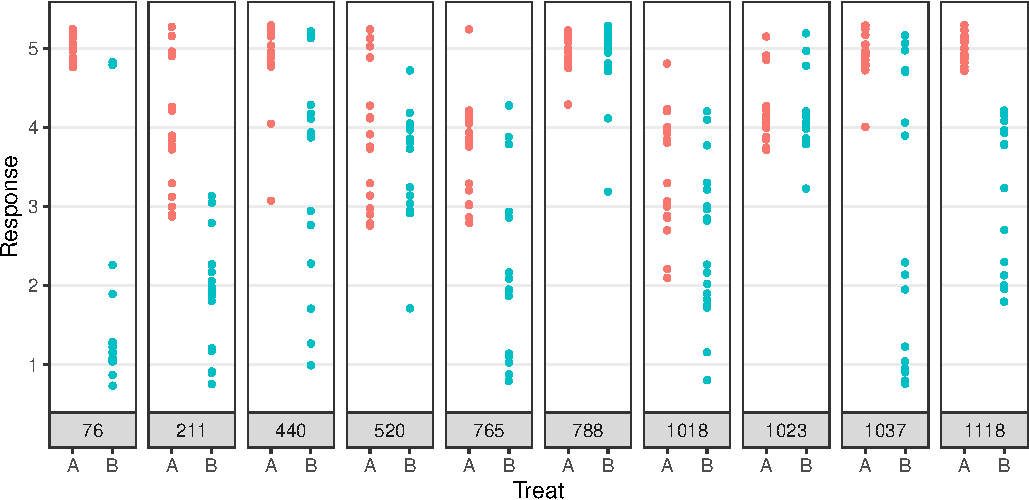
\includegraphics{4_files/figure-pdf/fig-subjects-1.pdf}

}

\caption{\label{fig-subjects}Respuestas de los estudiantes por nivel de
subtitulado.}

\end{figure}

\normalsize

\scriptsize

\begin{Shaded}
\begin{Highlighting}[]
\FunctionTok{options}\NormalTok{(}\AttributeTok{contrasts =} \FunctionTok{rep}\NormalTok{(}\StringTok{"contr.sum"}\NormalTok{, }\DecValTok{2}\NormalTok{))}
\NormalTok{clmm\_treat.period\_subject }\OtherTok{\textless{}{-}} \FunctionTok{clmm}\NormalTok{(}
\NormalTok{    Response }\SpecialCharTok{\textasciitilde{}}\NormalTok{ Treat }\SpecialCharTok{*}\NormalTok{ Period }\SpecialCharTok{+}\NormalTok{ (}\DecValTok{1} \SpecialCharTok{|}\NormalTok{ Subject),}
    \AttributeTok{data =}\NormalTok{ df\_response}
\NormalTok{)}
\FunctionTok{summary}\NormalTok{(clmm\_treat.period\_subject)}
\end{Highlighting}
\end{Shaded}

\begin{verbatim}
Cumulative Link Mixed Model fitted with the Laplace approximation

formula: Response ~ Treat * Period + (1 | Subject)
data:    df_response

 link  threshold nobs logLik   AIC     niter     max.grad cond.H 
 logit flexible  2980 -3655.71 7327.41 765(3046) 1.63e-03 8.1e+01

Random effects:
 Groups  Name        Variance Std.Dev.
 Subject (Intercept) 1.278    1.131   
Number of groups:  Subject 87 

Coefficients:
               Estimate Std. Error z value Pr(>|z|)    
Treat1          1.05368    0.03999  26.346  < 2e-16 ***
Period1         0.15662    0.03604   4.346 1.39e-05 ***
Treat1:Period1  0.14262    0.12677   1.125    0.261    
---
Signif. codes:  0 '***' 0.001 '**' 0.01 '*' 0.05 '.' 0.1 ' ' 1

Threshold coefficients:
    Estimate Std. Error z value
1|2  -3.7046     0.1523 -24.332
2|3  -2.0298     0.1349 -15.050
3|4  -1.1012     0.1310  -8.406
4|5   0.8281     0.1299   6.375
\end{verbatim}

\normalsize

En la parte de efectos fijos: los interceptos tienen valores similares
al modelo de efectos fijos (ver Sección~\ref{sec-response-treat.period})
aunque los coeficientes incrementan ligeramente su valor. Esto indica
una mayor distancia entre las respuestas de los subtitulados \(A\) y
\(B\). En este modelo el efecto secuencia no es significativo. En cuanto
a los efectos aleatorios: la varianza del intercepto aleatorio de los
estudiantes es 1.28. En la Figura~\ref{fig-random-subject-var} se
muestran los valores de los interceptos estimados de los estudiantes. La
media de estos interceptos como se espera es cercana a cero (-0.008).

\begin{figure}[h]

{\centering 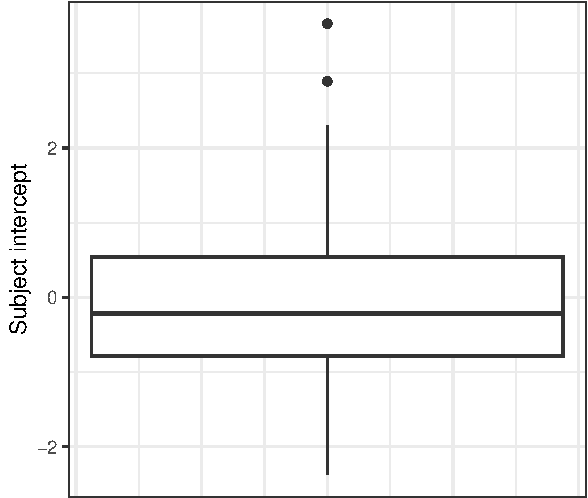
\includegraphics{4_files/figure-pdf/fig-random-subject-var-1.pdf}

}

\caption[Distribución de interceptos aleatorios por
estudiante.]{\label{fig-random-subject-var}Distribución de interceptos
aleatorios por estudiante en el modelo Response \textasciitilde{} Treat
* Period + (1 \textbar{} Subject)}

\end{figure}

\hypertarget{modelo-response-treat-period-1-treat-subject}{%
\subsubsection{Modelo Response \textasciitilde{} Treat * Period + (1 +
Treat \textbar{}
Subject)}\label{modelo-response-treat-period-1-treat-subject}}

Es posible que cada estudiante valore con diferente criterio cada
subtitulado. Para estimarlo, se propone el siguiente modelo:

\small

\[
\begin{aligned}
Nivel\ 1: & \text{logit}(P(Response_{ij} \leq k)) = \tau_{kj} - \beta_{1j} \text{Treat}_{ij} - \beta_{2} \text{Period}_{ij} - \beta_{3} \text{Treat}_{ij} * \text{Period}_{ij} \\
Nivel\ 2: & \tau_{kj}  =  \tau_{k} + Subject_{0j} \\
          & \beta_{1j}  =  \beta_{1} + Subject_{1j}
\end{aligned}
\]

\normalsize

Ahora el parámetro \(\beta_{1j}\) del subtitulado tiene dos componentes:
Uno común a todos los niveles de respuesta \(\beta_{1}\) y otro
particular de cada estudiante \(Subject_{1j}\). El modelo ajustado
ocasiona que solo \texttt{Treat1} sea significativo, ya que ni el
periodo ni la secuencia lo son. En los efectos aleatorios la correlación
entre intercepto y pendiente es prácticamente nula.

\scriptsize

\begin{Shaded}
\begin{Highlighting}[]
\FunctionTok{options}\NormalTok{(}\AttributeTok{contrasts =} \FunctionTok{rep}\NormalTok{(}\StringTok{"contr.sum"}\NormalTok{, }\DecValTok{2}\NormalTok{))}
\NormalTok{clmm\_treat.period\_treat.subject }\OtherTok{\textless{}{-}} \FunctionTok{clmm}\NormalTok{(}
\NormalTok{    Response }\SpecialCharTok{\textasciitilde{}}\NormalTok{ Treat }\SpecialCharTok{*}\NormalTok{ Period }\SpecialCharTok{+}\NormalTok{ (}\DecValTok{1} \SpecialCharTok{+}\NormalTok{ Treat }\SpecialCharTok{|}\NormalTok{ Subject),}
    \AttributeTok{data =}\NormalTok{ df\_response}
\NormalTok{)}
\FunctionTok{summary}\NormalTok{(clmm\_treat.period\_treat.subject)}
\end{Highlighting}
\end{Shaded}

\begin{verbatim}
Cumulative Link Mixed Model fitted with the Laplace approximation

formula: Response ~ Treat * Period + (1 + Treat | Subject)
data:    df_response

 link  threshold nobs logLik   AIC     niter     max.grad cond.H 
 logit flexible  2980 -3429.88 6879.76 905(6264) 1.33e-03 8.2e+01

Random effects:
 Groups  Name        Variance Std.Dev. Corr   
 Subject (Intercept) 1.712    1.308           
         Treat1      1.042    1.021    -0.062 
Number of groups:  Subject 87 

Coefficients:
               Estimate Std. Error z value Pr(>|z|)    
Treat1           1.2938     0.1197  10.809   <2e-16 ***
Period1          0.1620     0.1171   1.383    0.167    
Treat1:Period1   0.1327     0.1464   0.906    0.365    
---
Signif. codes:  0 '***' 0.001 '**' 0.01 '*' 0.05 '.' 0.1 ' ' 1

Threshold coefficients:
    Estimate Std. Error z value
1|2  -4.2633     0.1761 -24.210
2|3  -2.3321     0.1562 -14.932
3|4  -1.2656     0.1520  -8.324
4|5   0.9659     0.1509   6.400
\end{verbatim}

\normalsize

\hypertarget{comparaciuxf3n-de-modelos}{%
\subsubsection{Comparación de modelos}\label{comparaciuxf3n-de-modelos}}

Se pueden comparar los modelos con el test de razón de verosimilitud que
se realiza con la función \texttt{anova} del paquete \texttt{ordinal}
\autocite[ver][]{ordinalR}. Se comprueba que en este test resulta
significativamente mejor el último modelo:

\scriptsize

\begin{Shaded}
\begin{Highlighting}[]
\FunctionTok{anova}\NormalTok{(clmm\_treat.period\_subject, clmm\_treat.period\_treat.subject)}
\end{Highlighting}
\end{Shaded}

\begin{verbatim}
Likelihood ratio tests of cumulative link models:
 
                                formula:                                         
clmm_treat.period_subject       Response ~ Treat * Period + (1 | Subject)        
clmm_treat.period_treat.subject Response ~ Treat * Period + (1 + Treat | Subject)
                                link: threshold:
clmm_treat.period_subject       logit flexible  
clmm_treat.period_treat.subject logit flexible  

                                no.par    AIC  logLik LR.stat df Pr(>Chisq)    
clmm_treat.period_subject            8 7327.4 -3655.7                          
clmm_treat.period_treat.subject     10 6879.8 -3429.9  451.66  2  < 2.2e-16 ***
---
Signif. codes:  0 '***' 0.001 '**' 0.01 '*' 0.05 '.' 0.1 ' ' 1
\end{verbatim}

\normalsize

\hypertarget{elecciuxf3n-del-mejor-modelo}{%
\subsubsection{Elección del mejor
modelo}\label{elecciuxf3n-del-mejor-modelo}}

Se han comparado distintos modelos:

\begin{itemize}
\tightlist
\item
  Response \textasciitilde{} (1 \textbar{} Subject)
\item
  Response \textasciitilde{} (1 + Treat \textbar{} Subject)
\item
  Response \textasciitilde{} (1 + Treat \textbar{} Item)
\item
  Response \textasciitilde{} Treat + (1 + Treat \textbar{} Subject)
\item
  Response \textasciitilde{} Treat + (1 + Treat \textbar{} Item)
\item
  Response \textasciitilde{} Treat*Period + (1 + Treat \textbar{}
  Subject)
\item
  Response \textasciitilde{} Treat*Period + (1 + Treat \textbar{} Item)
\item
  Response \textasciitilde{} Treat*Period + (1 + Period \textbar{}
  Subject) + (1 + Treat \textbar{} Item)
\item
  Response \textasciitilde{} Treat + (1 + Treat \textbar{} Subject) + (1
  + Treat \textbar{} Item)
\item
  Response \textasciitilde{} Treat*Period + (1 + Treat \textbar{}
  Subject) + (1 + Treat \textbar{} Item)
\end{itemize}

El último de ellos produce un resultado significativo en el test de
razón de verosimilitud con todos los demás. Sin embargo los parámetros
de todos los modelos tienen valores similares por lo que no cambia la
interpretación que se haga de ellos en cada modelo. Este modelo tiene un
\(AIC\) menor que los modelos ordinales ajustados en el apartado
anterior (ver Sección~\ref{sec-ordinal-2}) incluso si a esos modelos se
les añade como factor predictor \texttt{Item}. Será este, por lo tanto,
el modelo seleccionado.

La Ecuación~\ref{eq-mejor-modelo} del modelo seleccionado es la
siguiente:

\small

\begin{equation}\protect\hypertarget{eq-mejor-modelo}{}{
\begin{aligned}
Nivel\ 1: & \text{logit}(P(Response_{ijl} \leq k)) = \tau_{kjl} - \beta_{1jl} \text{Treat}_{ijl} - \beta_{2} \text{Period}_{ijl} - \beta_{3} \text{Treat}_{ijl} * \text{Period}_{ijl} \\
Nivel\ 2: & \tau_{kjl}  =  \tau_{k} + Subject_{0j} + Item_{0l} \\
          & \beta_{1jl}  =  \beta_{1} + Subject_{1j} + Item_{1l}
\end{aligned}
}\label{eq-mejor-modelo}\end{equation}

\normalsize

donde \(ijl\) se corresponde con la observación \(i\)-ésima del
estudiante \(j\) e ítem \(l\). Ahora los interceptos y el coeficiente
del subtitulado se componen de tres sumandos: una parte fija, una parte
que depende del estudiante y una parte que depende del ítem de Likert.

El resumen de parámetros del modelo es el siguiente:

\scriptsize

\begin{Shaded}
\begin{Highlighting}[]
\FunctionTok{options}\NormalTok{(}\AttributeTok{contrasts =} \FunctionTok{rep}\NormalTok{(}\StringTok{"contr.sum"}\NormalTok{, }\DecValTok{2}\NormalTok{))}
\NormalTok{clmm\_treat.period.subject.item }\OtherTok{\textless{}{-}} \FunctionTok{clmm}\NormalTok{(}
\NormalTok{    Response }\SpecialCharTok{\textasciitilde{}}\NormalTok{ Treat }\SpecialCharTok{*}\NormalTok{ Period }\SpecialCharTok{+}\NormalTok{ (}\DecValTok{1} \SpecialCharTok{+}\NormalTok{ Treat }\SpecialCharTok{|}\NormalTok{ Subject) }\SpecialCharTok{+}\NormalTok{ (}\DecValTok{1} \SpecialCharTok{+}\NormalTok{ Treat }\SpecialCharTok{|}\NormalTok{ Item),}
    \AttributeTok{data =}\NormalTok{ df\_response}
\NormalTok{)}
\FunctionTok{summary}\NormalTok{(clmm\_treat.period.subject.item)}
\end{Highlighting}
\end{Shaded}

\begin{verbatim}
Cumulative Link Mixed Model fitted with the Laplace approximation

formula: Response ~ Treat * Period + (1 + Treat | Subject) + (1 + Treat |  
    Item)
data:    df_response

 link  threshold nobs logLik   AIC     niter       max.grad cond.H 
 logit flexible  2980 -3186.06 6398.11 1468(12273) 2.37e-03 1.5e+02

Random effects:
 Groups  Name        Variance Std.Dev. Corr   
 Subject (Intercept) 2.2176   1.4892          
         Treat1      1.3650   1.1683   -0.128 
 Item    (Intercept) 0.4831   0.6950          
         Treat1      0.4655   0.6823   -0.528 
Number of groups:  Subject 87,  Item 18 

Coefficients:
               Estimate Std. Error z value Pr(>|z|)    
Treat1           1.4320     0.2102   6.811  9.7e-12 ***
Period1          0.1730     0.1325   1.306    0.192    
Treat1:Period1   0.1397     0.1654   0.845    0.398    
---
Signif. codes:  0 '***' 0.001 '**' 0.01 '*' 0.05 '.' 0.1 ' ' 1

Threshold coefficients:
    Estimate Std. Error z value
1|2  -5.0033     0.2619 -19.104
2|3  -2.6499     0.2417 -10.962
3|4  -1.3659     0.2376  -5.748
4|5   1.1837     0.2365   5.006
\end{verbatim}

\normalsize

Con este modelo los efectos secuencia y periodo no son significativos.
En cualquier caso se mantienen ya que el test de razón de verosimilitud
resulta significativo en este modelo respecto al modelo sin estos
predictores.

\hypertarget{sec-bayesiano-2}{%
\subsection{Modelado bayesiano}\label{sec-bayesiano-2}}

Existen muchos paquetes en R para hacer inferencia bayesiana. Algunos de
los más populares son:

\begin{itemize}
\tightlist
\item
  OpenBUGS y WinBUGS: basado en el muestreo de Gibbs.
\item
  JAGS: también utiliza el muestreo de Gibbs.
\item
  Stan: Más moderno y con una comunidad de desarrollo más activa que los
  anteriores. Utiliza muestreo HMC (Hamiltonian Monte Carlo) y NUTS (no
  U-turn sampler). Stan tiene un lenguaje similar a C para definir
  modelos aunque hay muchos paquetes basados en Stan que facilitan la
  especificación de modelos con una sintaxis más sencilla. En este
  trabajo se utilizará uno de ellos, \texttt{brms}
  \autocite[ver][]{brms} . La sintaxis de especificación de modelos con
  este paquete es idéntica a la que se ha utilizado en la sección
  anterior.
\item
  INLA: Evita la simulación \emph{\gls{MCMC}} haciendo más rápida la
  convergencia. Es menos flexible ya que solo se pueden especificar
  modelos de la familia exponencial.
\end{itemize}

Se han comparado múltiples modelos usando la función \texttt{LOO} que
realiza una validación cruzada bayesiana \texttt{leave-one-out} similar
a la que se explicó en la Sección~\ref{sec-bayesiano}. El mejor modelo
ha resultado ser el mismo que se seleccionó en modelos mixtos (ver
Ecuación~\ref{eq-mejor-modelo}). Es decir:

\small

\begin{quote}
Response \textasciitilde{} Treat*Period + (1 + Treat \textbar{} Subject)
+ (1 + Treat \textbar{} Item) \normalsize
\end{quote}

\scriptsize

\begin{Shaded}
\begin{Highlighting}[]
\FunctionTok{options}\NormalTok{(}\AttributeTok{contrasts =} \FunctionTok{rep}\NormalTok{(}\StringTok{"contr.sum"}\NormalTok{, }\DecValTok{2}\NormalTok{))}
\NormalTok{brm\_treat.period.subject.item }\OtherTok{\textless{}{-}} \FunctionTok{brm}\NormalTok{(}
\NormalTok{    Response }\SpecialCharTok{\textasciitilde{}}\NormalTok{ Treat }\SpecialCharTok{*}\NormalTok{ Period }\SpecialCharTok{+}\NormalTok{ (}\DecValTok{1} \SpecialCharTok{+}\NormalTok{ Treat }\SpecialCharTok{|}\NormalTok{ Subject) }\SpecialCharTok{+}\NormalTok{ (}\DecValTok{1} \SpecialCharTok{+}\NormalTok{ Treat }\SpecialCharTok{|}\NormalTok{ Item),}
    \AttributeTok{data =}\NormalTok{ df\_response,}
    \AttributeTok{family =} \FunctionTok{cumulative}\NormalTok{(}\StringTok{"logit"}\NormalTok{),}
    \AttributeTok{iter =} \DecValTok{4000}\NormalTok{,}
    \AttributeTok{sample\_prior =} \ConstantTok{TRUE}\NormalTok{,}
    \AttributeTok{file =} \StringTok{"models/brm\_treat.period.subject.item"}\NormalTok{,}
    \AttributeTok{file\_refit =} \StringTok{"on\_change"}
\NormalTok{)}
\end{Highlighting}
\end{Shaded}

\normalsize

El modelo utiliza como factores con efectos fijos
(\texttt{complete\ pooling} en terminología bayesiana) el nivel de
subtitulado y el periodo y la interacción entre ambos; y como efectos
aleatorios (\texttt{partial\ pooling}) los sujetos y los ítems del test,
cada uno de ellos con un intercepto y un nivel de subtitulado variable.
El resumen del modelo es el siguiente:

\tiny

\begin{Shaded}
\begin{Highlighting}[]
\FunctionTok{summary}\NormalTok{(brm\_treat.period.subject.item)}
\end{Highlighting}
\end{Shaded}

\begin{verbatim}
 Family: cumulative 
  Links: mu = logit; disc = identity 
Formula: Response ~ Treat * Period + (1 + Treat | Subject) + (1 + Treat | Item) 
   Data: df_response (Number of observations: 2980) 
  Draws: 4 chains, each with iter = 4000; warmup = 2000; thin = 1;
         total post-warmup draws = 8000

Group-Level Effects: 
~Item (Number of levels: 18) 
                      Estimate Est.Error l-95% CI u-95% CI Rhat Bulk_ESS
sd(Intercept)             0.77      0.16     0.53     1.15 1.00     1468
sd(Treat1)                0.77      0.15     0.53     1.12 1.00     1935
cor(Intercept,Treat1)    -0.46      0.20    -0.78     0.01 1.00     1421
                      Tail_ESS
sd(Intercept)             2605
sd(Treat1)                3580
cor(Intercept,Treat1)     2555

~Subject (Number of levels: 87) 
                      Estimate Est.Error l-95% CI u-95% CI Rhat Bulk_ESS
sd(Intercept)             1.54      0.14     1.29     1.85 1.00     1484
sd(Treat1)                1.21      0.11     1.01     1.45 1.00     1519
cor(Intercept,Treat1)    -0.11      0.12    -0.34     0.14 1.00     1228
                      Tail_ESS
sd(Intercept)             2741
sd(Treat1)                3081
cor(Intercept,Treat1)     2475

Population-Level Effects: 
               Estimate Est.Error l-95% CI u-95% CI Rhat Bulk_ESS Tail_ESS
Intercept[1]      -4.95      0.28    -5.52    -4.42 1.00      785     1753
Intercept[2]      -2.59      0.26    -3.11    -2.09 1.01      743     1636
Intercept[3]      -1.30      0.26    -1.82    -0.82 1.01      726     1532
Intercept[4]       1.25      0.26     0.74     1.75 1.00      745     1571
Treat1             1.46      0.23     1.01     1.92 1.00     1046     2071
Period1            0.17      0.14    -0.09     0.44 1.00      848     1714
Treat1:Period1     0.14      0.17    -0.20     0.47 1.01      686     1127

Family Specific Parameters: 
     Estimate Est.Error l-95% CI u-95% CI Rhat Bulk_ESS Tail_ESS
disc     1.00      0.00     1.00     1.00   NA       NA       NA

Draws were sampled using sampling(NUTS). For each parameter, Bulk_ESS
and Tail_ESS are effective sample size measures, and Rhat is the potential
scale reduction factor on split chains (at convergence, Rhat = 1).
\end{verbatim}

\normalsize

Se han mantenido las distribuciones de probabilidad a priori que por
defecto utiliza \texttt{brm} confiando en que sus parámetros son
adecuados. Sin embargo, conviene comprobar que realmente sea así. En la
Tabla~\ref{tbl-priors} se muestran las distribuciones a priori de los
parámetros aleatorios del modelo. En la Figura~\ref{fig-priors} se
constata que toman valores razonables y no informativos.

\tiny

\hypertarget{tbl-priors}{}
\begin{longtable}{llllrrrrrl}
\caption{\label{tbl-priors}Distribuciones a priori del modelo ordinal seleccionado. }\tabularnewline

\toprule
prior & class & coef & group & resp & dpar & nlpar & lb & ub & source \\ 
\midrule
 & b &  &  &  &  &  &  &  & default \\ 
 & b & Period1 &  &  &  &  &  &  & default \\ 
 & b & Treat1 &  &  &  &  &  &  & default \\ 
 & b & Treat1:Period1 &  &  &  &  &  &  & default \\ 
student\_t(3, 0, 2.5) & Intercept &  &  &  &  &  &  &  & default \\ 
student\_t(3, 0, 2.5) & Intercept & 1 &  &  &  &  &  &  & default \\ 
student\_t(3, 0, 2.5) & Intercept & 2 &  &  &  &  &  &  & default \\ 
student\_t(3, 0, 2.5) & Intercept & 3 &  &  &  &  &  &  & default \\ 
student\_t(3, 0, 2.5) & Intercept & 4 &  &  &  &  &  &  & default \\ 
lkj\_corr\_cholesky(1) & L &  &  &  &  &  &  &  & default \\ 
lkj\_corr\_cholesky(1) & L &  & Item &  &  &  &  &  & default \\ 
lkj\_corr\_cholesky(1) & L &  & Subject &  &  &  &  &  & default \\ 
student\_t(3, 0, 2.5) & sd &  &  &  &  &  & 0 &  & default \\ 
student\_t(3, 0, 2.5) & sd &  & Item &  &  &  &  &  & default \\ 
student\_t(3, 0, 2.5) & sd & Intercept & Item &  &  &  &  &  & default \\ 
student\_t(3, 0, 2.5) & sd & Treat1 & Item &  &  &  &  &  & default \\ 
student\_t(3, 0, 2.5) & sd &  & Subject &  &  &  &  &  & default \\ 
student\_t(3, 0, 2.5) & sd & Intercept & Subject &  &  &  &  &  & default \\ 
student\_t(3, 0, 2.5) & sd & Treat1 & Subject &  &  &  &  &  & default \\ 
\bottomrule
\end{longtable}

\normalsize

\begin{figure}[h]

{\centering 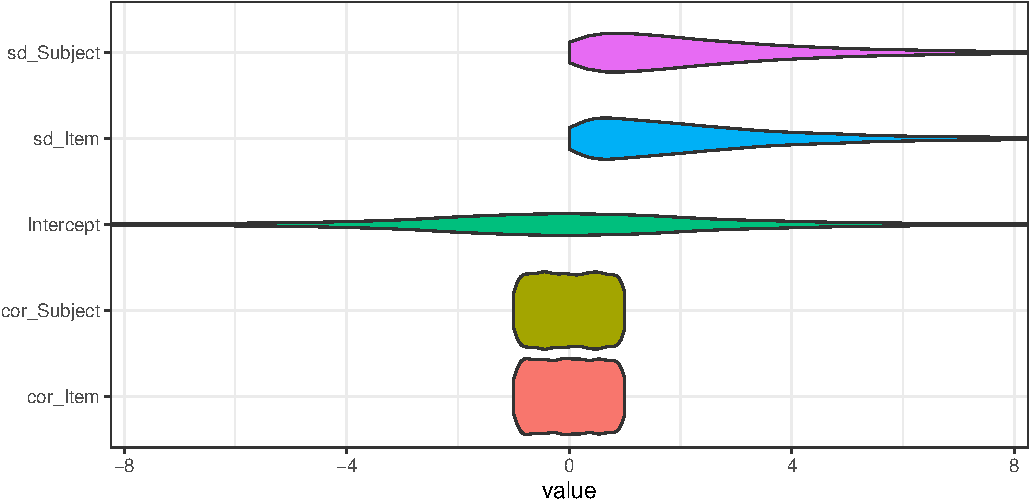
\includegraphics{4_files/figure-pdf/fig-priors-1.pdf}

}

\caption[Distribuciones a priori del modelo
seleccionado.]{\label{fig-priors}Distribuciones a priori del modelo
Response \textasciitilde{} Treat * Period + (1 + Treat \textbar{}
Subject) + (1 + Treat \textbar{} Item).}

\end{figure}

Es importante asegurar que el entrenamiento ha convergido a su
distribución a posteriori. En la tabla de resumen se constata que el
valor de \texttt{Rhat} \footnote{\texttt{Rhat} es una medida utilizada
  para evaluar la convergencia de las Cadenas de Markov Monte Carlo
  (\(MCMC\)) en el muestreo bayesiano. Compara la varianza de cada
  cadena individual de \(MCMC\) con la varianza entre diferentes
  cadenas. Si las cadenas convergen, se espera que sus valores sean
  similares y, por lo tanto, el valor de \texttt{Rhat} será próximo a 1.}
es inferior a 1.1 y el de \texttt{ESS} \footnote{\texttt{ESS} (Efficient
  Sample Size) es una estimación del número de muestras independientes
  obtenidas en el muestreo \(MCMC\).} superior a 400 en todos los
parámetros, que son umbrales que no se deberían violar
\autocite[ver][]{burkner2019}. En la Figura~\ref{fig-trace} se comprueba
que las cadenas \(MCMC\) de muestreo de la distribución a posteriori se
mezclan correctamente y no se aprecia autocorrelación en ninguno de los
parámetros. Por último, en la Figura~\ref{fig-predictive} se muestra una
comparación entre los histogramas construidos con los datos de las
respuestas a los test con los intervalos de credibilidad marginales de
la función predictiva a posteriori del modelo. En la mayoría de los
ítems, el muestreo se ajusta bastante bien al histograma de respuestas;
aunque en algunos ítems, como el \texttt{Q16} o el \texttt{Q17}, se
aprecian diferencias relevantes.

\begin{figure}[h]

{\centering 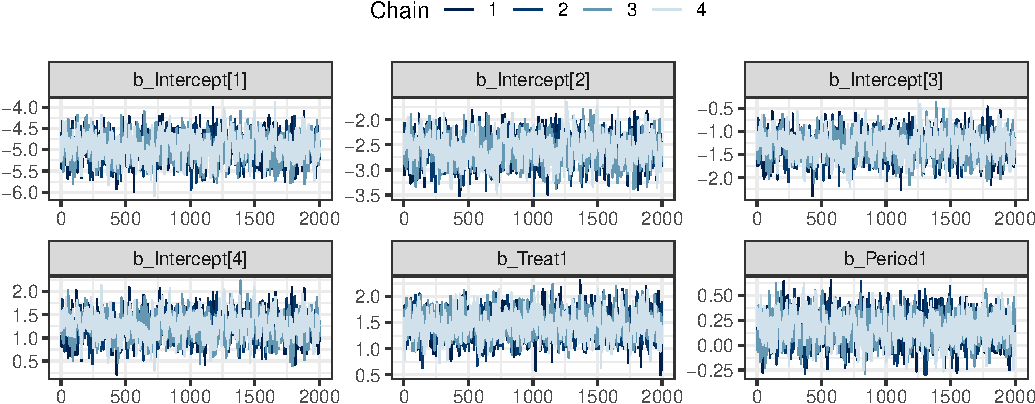
\includegraphics{4_files/figure-pdf/fig-trace-1.pdf}

}

\caption[Cadenas MCMC del modelo seleccionado.]{\label{fig-trace}Cadenas
MCMC del modelo Response \textasciitilde{} Treat * Period + (1 + Treat
\textbar{} Subject) + (1 + Treat \textbar{} Item).}

\end{figure}

\begin{figure}[h]

{\centering 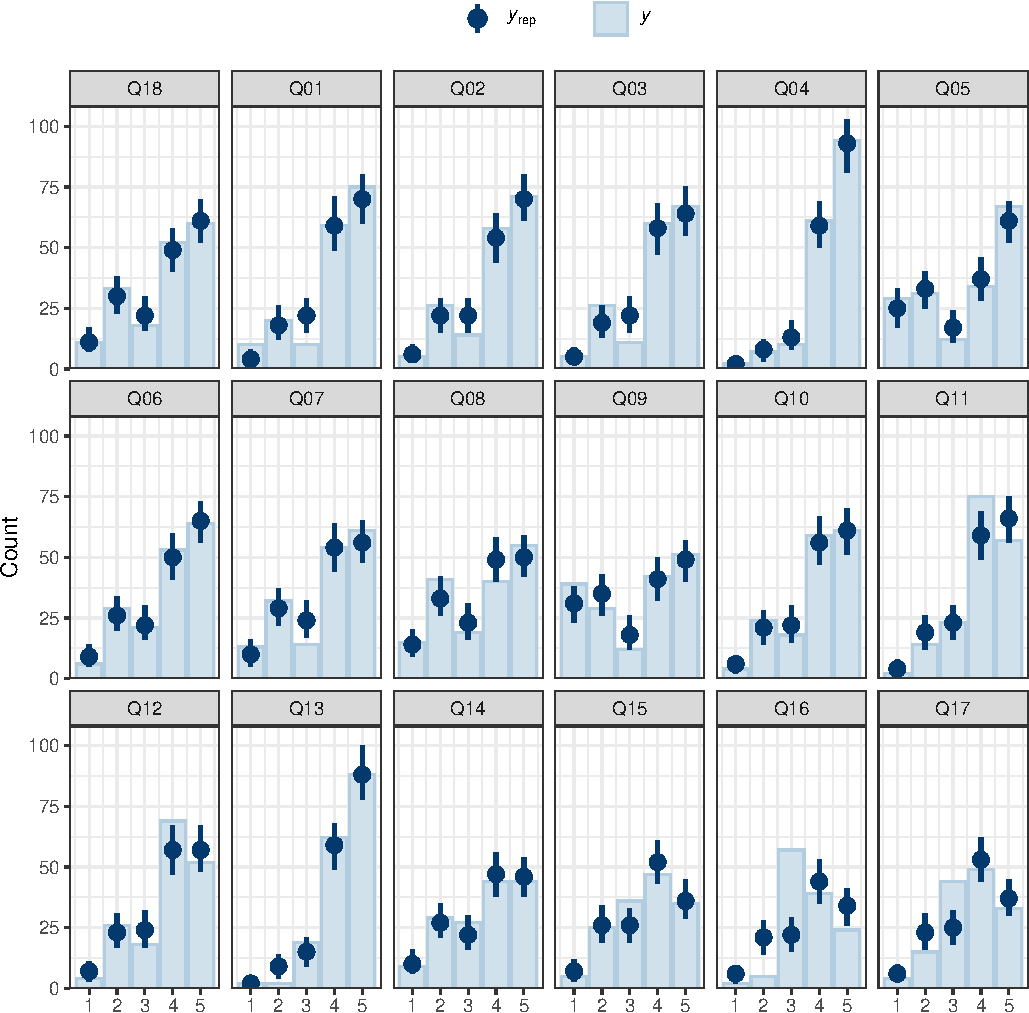
\includegraphics{4_files/figure-pdf/fig-predictive-1.pdf}

}

\caption[Verificación usando la función predictiva a posteriori del
modelo seleccionado.]{\label{fig-predictive}Comparación de los valores
reales con los obtenidos a partir de la función predictiva a posteriori
del modelo Response \textasciitilde{} Treat * Period + (1 + Treat
\textbar{} Subject) + (1 + Treat \textbar{} Item).}

\end{figure}

\bookmarksetup{startatroot}

\hypertarget{sec-resultados}{%
\chapter{Resultados}\label{sec-resultados}}

En el Capítulo~\ref{sec-modelado} se realizó una exploración de los
datos y se adecuaron los modelos presentados en el
Capítulo~\ref{sec-arte} al diseño del experimento del subtitulado. En
este capítulo se comentan los resultados de los modelos seleccionados
siguiendo el mismo orden expositivo, comenzando por el análisis del
\gls{OR}, continuando por la \gls{Regresión Logística} y finalizando con
la \gls{Regresión Ordinal}.

\hypertarget{sec-or-3}{%
\subsection{\texorpdfstring{Comparación con \emph{Odds
Ratio}}{Comparación con Odds Ratio}}\label{sec-or-3}}

El contraste de hipótesis del \(log\ OR\) del nivel subtitulado y
secuencia (ver Sección~\ref{sec-or-2}) no produce significación
estadística en ningún nivel de respuesta, por lo que según esta prueba
estadística el orden en el que se ven los vídeos no influiría en la
respuesta de los estudiantes (ver Tabla~\ref{tbl-logor1}).

\hypertarget{tbl-logor1}{}
\begin{longtable}{lrrrr}
\caption{\label{tbl-logor1}Log OR \textasciitilde{} Treat + Seq + Response }\tabularnewline

\toprule
Response & Estimate & Std. Error & z value & Pr(>|z|) \\ 
\midrule
No sé / No contesto & 0.190 & 0.327 & 0.580 & 0.562 \\ 
Muy en desacuerdo & -0.135 & 1.012 & -0.134 & 0.894 \\ 
En desacuerdo & -0.244 & 0.291 & -0.838 & 0.402 \\ 
Neutral & 0.152 & 0.214 & 0.711 & 0.477 \\ 
De acuerdo & -0.210 & 0.134 & -1.570 & 0.116 \\ 
Muy de acuerdo & 0.117 & 0.137 & 0.855 & 0.393 \\ 
\bottomrule
\end{longtable}

Sin embargo, si se realiza este contraste entre subtítulos y periodos,
se constata la existencia de un \gls{efecto periodo} de signo contrario
para los ítems 4 y 5 (ver Tabla~\ref{tbl-logor2}). El test es
significativo porque el ratio entre subtítulos de respuestas con valor 4
es diferente en cada periodo habiendo mayor cantidad de respuestas 4 en
el segundo periodo que en el primero. Con las respuestas 5 ocurre lo
contrario: la proporción es mayor en el primer periodo. La
Figura~\ref{fig-or2} permite una comprobación visual. Esto indica que
los estudiantes de ambos grupos prestaron más atención o fueron más
exigentes en el segundo visionado y valoraron relativamente peor el
segundo vídeo. Que el efecto periodo sea de signo contrario en dos
respuestas no debe sorprender en este diseño de experimento, ya que un
test es un juego de suma cero: la valoraciones que se ganan o se pierden
en un nivel de respuesta necesariamente se reparten entre el resto de
niveles. En cualquier caso, el efecto periodo es cuantitativa y
cualitativamente pequeño. Al afectar solo al intercambio de valoraciones
entre los niveles 4 y 5 es simplemente una pequeña corrección en la
valoración del subtitulado y cualitativamente es poco importante ya que
las respuestas 4 y 5 son ambas valoraciones positivas.

\hypertarget{tbl-logor2}{}
\begin{longtable}{lrrrr}
\caption{\label{tbl-logor2}Log OR \textasciitilde{} Treat + Period + Response }\tabularnewline

\toprule
Response & Estimate & Std. Error & z value & Pr(>|z|) \\ 
\midrule
No sé / No contesto & 0.335 & 0.327 & 1.022 & 0.307 \\ 
Muy en desacuerdo & 0.135 & 1.012 & 0.134 & 0.894 \\ 
En desacuerdo & -0.121 & 0.291 & -0.416 & 0.677 \\ 
Neutral & 0.055 & 0.214 & 0.259 & 0.796 \\ 
De acuerdo & -0.851 & 0.134 & -6.367 & 0.000 \\ 
Muy de acuerdo & 0.486 & 0.137 & 3.557 & 0.000 \\ 
\bottomrule
\end{longtable}

\begin{figure}[h]

{\centering 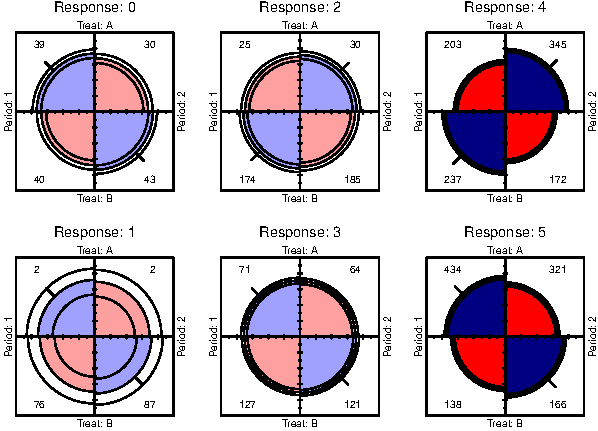
\includegraphics{5_files/figure-pdf/fig-or2-1.pdf}

}

\caption[Test Odds Ratio \textasciitilde{} Treat + Period +
Response]{\label{fig-or2}OR \textasciitilde{} Treat + Period + Response}

\end{figure}

\hypertarget{modelado}{%
\subsection{Modelado}\label{modelado}}

\hypertarget{sec-logistica-3}{%
\subsubsection{Regresión Logística}\label{sec-logistica-3}}

En la Sección~\ref{sec-logistica-2} se explicó una forma de crear una
variable dicotómica que permite ajustar los datos a una Regresión
Logística. Concretamente, se creó la variable respuesta \(Improve\) que
compara si las respuestas de cada estudiante a cada Ítem entre los
niveles de subtitulado (\(A\) frente \(B\)) han mejorado (valor 1) o se
han mantenido o empeorado (valor 0). El modelo que se propone en esta
sección no tiene en cuenta el \gls{efecto secuencia} ya que resultó no
significativo en el análisis y, en cambio, se incluye como efectos
aleatorios los estudiantes y los ítems sobre el intercepto ya que, como
se ha explicado, son variables que no se pueden considerar
independientes:

\begin{quote}
Improve \textasciitilde{} 1 + (1 \textbar{} Subject) + (1 \textbar{}
Item)
\end{quote}

\scriptsize

\begin{Shaded}
\begin{Highlighting}[]
\NormalTok{glmer\_improve\_subject\_question }\OtherTok{\textless{}{-}} \FunctionTok{glmer}\NormalTok{(}
\NormalTok{    Improve }\SpecialCharTok{\textasciitilde{}} \DecValTok{1} \SpecialCharTok{+}\NormalTok{ (}\DecValTok{1} \SpecialCharTok{|}\NormalTok{ Subject) }\SpecialCharTok{+}\NormalTok{ (}\DecValTok{1} \SpecialCharTok{|}\NormalTok{ Item),}
    \AttributeTok{family =} \StringTok{"binomial"}\NormalTok{, }\AttributeTok{data =}\NormalTok{ df\_improve}
\NormalTok{)}
\end{Highlighting}
\end{Shaded}

\normalsize

El resumen del modelo ajustado con la función \texttt{glmer} del paquete
\texttt{lme4} \autocite[ver][]{lme4} produce los resultados de la
columna izquierda de la Tabla~\ref{tbl-selected-logistic}. El intercepto
del modelo ajustado es 0.404 (std.error 0.329). Por ello, la
probabilidad de que se otorgue una mayor puntuación en \(A\) que en
\(B\) es del 59.95\%. La proporción de varianza explicada por los
efectos aleatorios (\emph{\gls{ICC}}) es 0.575.

\hypertarget{tbl-selected-logistic}{}
\begin{table}
\caption{\label{tbl-selected-logistic}Resumen de los modelos de Regresión Logística. }\tabularnewline

\centering
\begin{tabular}[t]{lcc}
\toprule
  & Improve (A>B) & Level == 'Positivo'\\
\midrule
(Intercept) & \num{0.404} & \num{1.474}\\
 & (\num{0.329}) & (\num{0.284})\\
Treat1 &  & \num{1.548}\\
 &  & (\num{0.223})\\
SD (Intercept Subject) & \num{1.832} & \num{1.590}\\
SD (Treat1 Subject) &  & \num{1.082}\\
Cor (Intercept\textasciitilde{}Treat1 Subject) &  & \num{-0.093}\\
SD (Intercept Item) & \num{1.051} & \num{0.893}\\
SD (Treat1 Item) &  & \num{0.726}\\
Cor (Intercept\textasciitilde{}Treat1 Item) &  & \num{-0.119}\\
\midrule
Num.Obs. & \num{1152} & \num{2980}\\
AIC & \num{1215.6} & \num{2390.0}\\
BIC & \num{1230.8} & \num{2438.0}\\
\bottomrule
\end{tabular}
\end{table}

Una forma alternativa de Regresión Logística es simplemente saber si
cada respuesta es positiva (4 ó 5) frente a si es negativa o neutra (1,
2, ó 3). Como efecto fijo se incorpora el nivel de subtitulado y como
efectos aleatorios el estudiante y el ítem ambos con intercepto y
pendiente sobre el subtitulado variables por tener mejor valor de
\(AIC\). La fórmula del modelo es la siguiente:

\small

\begin{quote}
I(Level == \enquote{Positivo}) \textasciitilde{} Treat + (1 + Treat
\textbar{} Subject) + (1 + Treat \textbar{} Item)
\end{quote}

\normalsize

En la columna derecha de la Tabla~\ref{tbl-selected-logistic} se muestra
el resumen del modelo. En este caso, el intercepto tiene una valor de
1.474. Por lo que la probabilidad de respuesta positiva en cualquier
ítem y nivel de subtitulado es 81.4\%. El coeficiente \texttt{Treat1}
tiene valor 1.548 y es el valor en \texttt{logits} que se añade o se
quita en función de si el subtitulado es el \(A\) o el \(B\). Esto se
traduce en que la posibilidad de una respuesta positiva en el
subtitulado \(A\) es 95.4\%. En el subtitulado \(B\) esta probabilidad
se reduce a 48.2\%. Por último, el valor de \(ICC\) del modelo es 0.604

\hypertarget{sec-ordinal-3}{%
\subsubsection{Regresión Ordinal}\label{sec-ordinal-3}}

En la Sección~\ref{sec-ordinal-2} se evaluaron distintas
parametrizaciones de la Regresión Ordinal Acumulativa tanto desde el
punto de vista frecuentista como bayesiano, considerando únicamente
efectos fijos y también efectos aleatorios. Finalmente, tanto en el
análisis frecuentista como en el bayesiano, el modelo que resultó ser
más parsimonioso (evaluado con \emph{\gls{LRT}} y con \(AIC\)) es el de
la Ecuación~\ref{eq-mejor-modelo}, que se reproduce aquí en sintaxis R:

\small

\begin{quote}
Response \textasciitilde{} Treat*Period + (1 + Treat \textbar{} Subject)
+ (1 + Treat \textbar{} Item)
\end{quote}

\normalsize

Este modelo incluye como efectos fijos el nivel de subtitulado
(\texttt{Treat}), el periodo (\texttt{Period}) y su interacción; y como
efectos aleatorios el estudiante (\texttt{Subject}) y el ítem
(\texttt{Item}). Ambos con interceptos y pendientes variables por nivel
de subtítulo. Los coeficientes estimados son muy similares tanto en el
paradigma frecuentista como en el bayesiano. En la
Tabla~\ref{tbl-model-comp} se comparan las estimaciones producidas por
ambos modelos. Como ya se dijo, el efecto más importante es el debido al
subtitulado (coeficiente frecuentista 1.432). En comparación con él, los
efectos debido al periodo y la secuencia son muy pequeños (coeficientes
0.173 y 0.14 respectivamente). La proporción de la varianza explicada
debida a efectos aleatorios (\(ICC\)) es 0.579.

En la Figura~\ref{fig-probs-clmm_treat.period.subject.question} se
muestran las predicciones del modelo por nivel de subtítulo y periodo.
El modelo predice para el subtitulado \(B\) el nivel 4 de respuesta como
el más probable seguido del 3, mientras para el subtitulado \(A\) el
nivel de respuesta más probable es el 5 seguido del 4. En el subtitulado
\(B\) apenas hay diferencias entre periodos, sin embargo, en el
subtitulado \(A\) hay mayor probabilidad del nivel de respuesta 5 en el
periodo 1 y nivel de respuesta 4 en el periodo 2.

\begin{figure}[h]

{\centering 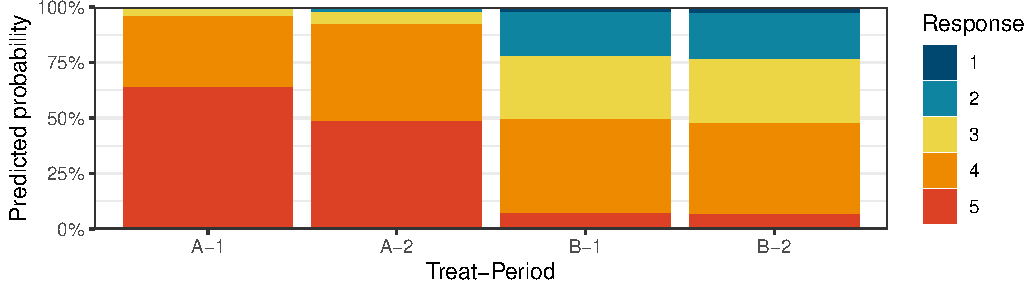
\includegraphics{5_files/figure-pdf/fig-probs-clmm_treat.period.subject.question-1.pdf}

}

\caption[Probabilidades de respuesta para el modelo ordinal
seleccionado.]{\label{fig-probs-clmm_treat.period.subject.question}Probabilidades
de respuesta para el modelo ordinal Response \textasciitilde{} Treat *
Period + (1 + Treat \textbar{} Subject) + (1 + Treat \textbar{} Item)}

\end{figure}

\tiny

\hypertarget{tbl-model-comp}{}
\begin{longtable}{lrrrrrr}
\caption{\label{tbl-model-comp}Comparación frecuentista/bayesiano de coeficientes estimados en el
modelo ordinal. }\tabularnewline

\toprule
 & \multicolumn{3}{c}{ordinal::clmm} & \multicolumn{3}{c}{brms::brm} \\ 
\cmidrule(lr){2-4} \cmidrule(lr){5-7}
Name & Estimation.clmm & conf.2.5\% & conf.97.5\% & Estimation.brm & cred.2.5\% & cred.97.5\% \\ 
\midrule
1|2 & -5.00 & -5.52 & -4.49 & -4.94 & -5.52 & -4.42 \\ 
2|3 & -2.65 & -3.12 & -2.18 & -2.58 & -3.11 & -2.09 \\ 
3|4 & -1.37 & -1.83 & -0.90 & -1.30 & -1.82 & -0.82 \\ 
4|5 & 1.18 & 0.72 & 1.65 & 1.25 & 0.74 & 1.75 \\ 
Treat1 & 1.43 & 1.02 & 1.84 & 1.46 & 1.01 & 1.92 \\ 
Period1 & 0.17 & -0.09 & 0.43 & 0.17 & -0.09 & 0.44 \\ 
Treat1:Period1 & 0.14 & -0.18 & 0.46 & 0.14 & -0.20 & 0.47 \\ 
Item.sd(Intercept) & 0.70 &  &  & 0.75 & 0.53 & 1.15 \\ 
Item.sd(Treat1) & 0.68 &  &  & 0.75 & 0.53 & 1.12 \\ 
Subject.sd(Intercept) & 1.49 &  &  & 1.53 & 1.29 & 1.85 \\ 
Subject.sd(Treat1) & 1.17 &  &  & 1.21 & 1.01 & 1.45 \\ 
Item.cor(Intercept,Treat1) & -0.53 &  &  & -0.49 & -0.78 & 0.01 \\ 
Subject.cor(Intercept,Treat1) & -0.13 &  &  & -0.11 & -0.34 & 0.14 \\ 
\bottomrule
\end{longtable}

\normalsize

En la Figura~\ref{fig-pred-3} se representan 50 muestras de la esperanza
de la distribución predictiva a posteriori para cada ítem y nivel de
subtitulado marginalizados por periodo y estudiante. La primera
conclusión que se puede extraer es que el modelo tiene bastante
incertidumbre sobre los valores de respuesta a cada ítem no superando
casi nunca el 50\% de probabilidad para todos los ítems y niveles de
subtitulado. En general se observa en la mayoría de los ítems del nivel
de subtitulado \(A\) que los alumnos están bastante seguros de que la
respuesta a los ítems debe ser 4 ó 5, asignando una muy baja
probabilidad a los valores 1, 2, ó 3, pero habiendo bastante
incertidumbre respecto cuál de los dos valores (4 ó 5) asignar. En el
nivel de subtitulado \(B\) la situación es bastante más confusa. Aunque
la opción de respuesta preferida es 4 y las menos preferidas son la 5 y
la 1, hay bastante mezcla entre las opciones de respuesta 2, 3 y 4. En
cuanto al análisis individualizado por ítem se llega a las siguientes
conclusiones:

\begin{itemize}
\item
  En los ítems \(Q04\) y \(Q13\) los estudiantes no aprecian defectos en
  el subtitulado ni diferencias entre un nivel y otro. Son valoradas en
  ambos subtitulados con puntuaciones de 4 y de 5.
\item
  En los ítems \(Q15\), \(Q16\) y \(Q17\), la opción de respuesta más
  probable es 4. El modelo asigna una baja probabilidad de respuesta a
  la opción 1 y similares al resto. La probabilidad de la opción 5
  decrece ligeramente entre subtitulado \(A\) y \(B\) y lo contrario
  ocurre con las opciones 2 y 3.
\item
  Los ítems \(Q01\), \(Q02\), \(Q03\), \(Q10\), \(Q11\) y \(Q12\) son
  similares a las anteriores. Particularmente en lo referente a que la
  respuesta más probable en el subtitulado \(B\) es 4. En el subtitulado
  \(A\) hay preferencia por 4 y 5. El nivel 5 cae acusadamente en el
  subtitulado \(B\) y en este nivel aumenta ligeramente la probabilidad
  de respuesta 2 y 3.
\item
  Los ítems \(Q06\), \(Q07\), \(Q14\) y \(Q18\) no son muy diferentes de
  los anteriores. En general el modelo predice mayor probabilidad de
  respuesta para 5 en el subtitulado \(A\) pero este valor es con alta
  probabilidad cercano a cero en el subtitulado \(B\). En el subtitulado
  \(B\) la probabilidad de respuesta 2, 3 ó 4 es similar.
\item
  Los ítems \(Q05\), \(Q08\) y \(Q09\) son los que más diferencias entre
  subtitulados presentan. La respuesta más probable en el subtitulado
  \(A\) es 5 (en \(Q08\) y en \(Q09\) muy parecida a 4). Por contra, en
  el subtitulado \(B\) las respuestas 4 y 5 tienden a cero, siendo la
  más probable la respuesta 2. En los ítems \(Q05\) y \(Q09\) la segunda
  respuesta más probable al subtitulado \(B\) es 1 y 4 en el ítem
  \(Q08\).
\end{itemize}

En definitiva, nuestro modelo predice que los estudiantes están bastante
de acuerdo en que en los ítems \(Q05\) y \(Q09\) hay una diferencia de
calidad importante entre subtitulados. También están de acuerdo en que
en los ítems \(Q04\) y \(Q13\) no hay apenas cambio entre los
subtitulados. En los ítems \(Q15\), \(Q16\) y \(Q17\) hay una gran
confusión en ambos niveles de subtitulado predominando la respuesta 4 y
siendo muy parecidas las respuestas en ambos niveles. En el resto la
confusión se circunscribe al nivel de subtitulado \(B\), ya que en el
nivel \(A\) las opciones 4 y 5 predominan.

\begin{figure}[h]

{\centering 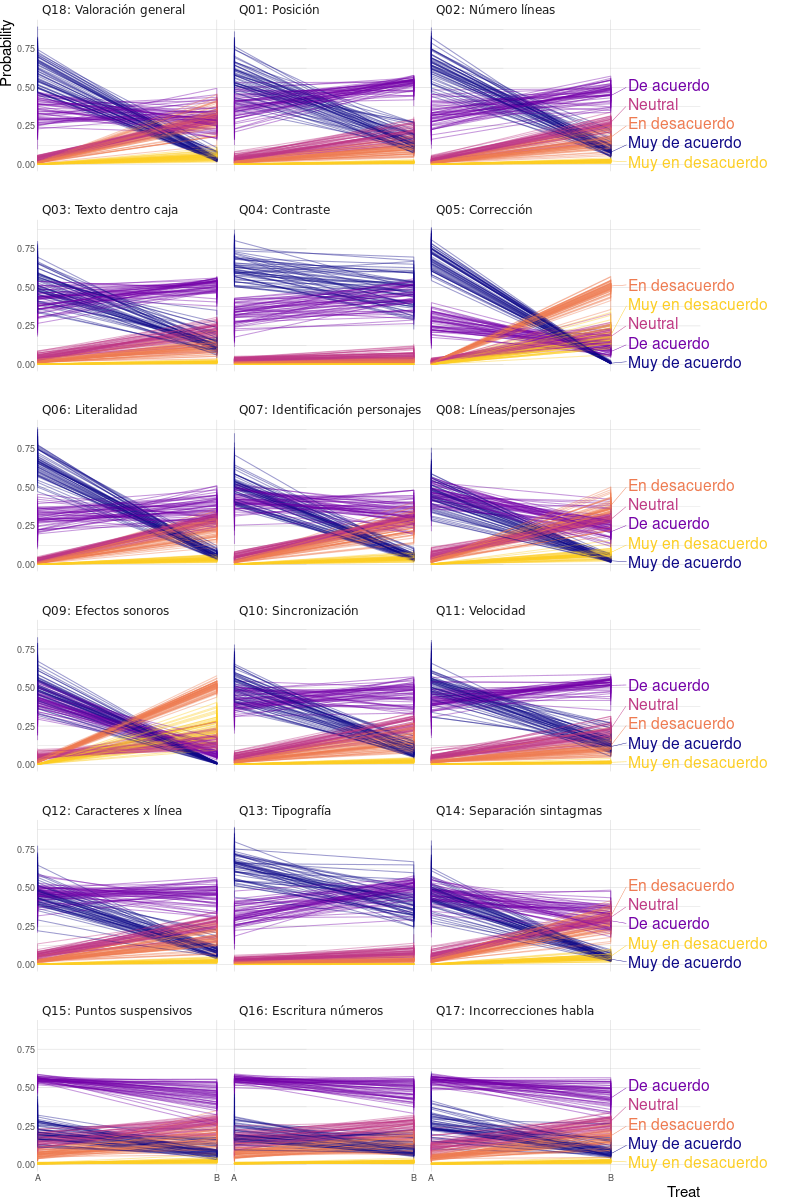
\includegraphics[width=1\textwidth,height=\textheight]{images/bayes-preg.png}

}

\caption{\label{fig-pred-3}Muestreo de la función predictiva a
posteriori por tratamiento e ítem.}

\end{figure}

\bookmarksetup{startatroot}

\hypertarget{sec-discusion}{%
\chapter{Discusión}\label{sec-discusion}}

\scriptsize

\normalsize

En esta sección se discuten los resultados una vez \enquote{descubierto
el ciego} y se responden a la pregunta de investigación y objetivos
específicos planteados en la Sección~\ref{sec-objetivos}. Se reveló que
el subtitulado que en este trabajo se ha denominado \(A\) se corresponde
que el vídeo correctamente subtitulado. Adicionalmente se ha
suministrado un documento que contiene los errores introducidos en el
subtitulado \(B\). A partir del mismo, se ha elaborado la Tabla
\ref{tbl-blind-errors} en la que se muestra la correspondencia de cada
error con los ítems de la \gls{escala de likert} a la que respondieron
los estudiantes (ver en la Tabla~\ref{tbl-likert-scale} una descripción
textual de cada ítem). Para 7 de los 18 ítems (Q01, Q03, Q04, Q13, Q15,
Q16, Q17) no se ha encontrado una adscripción clara en el documento de
errores y, por lo tanto, sería esperable que las respuestas de los
estudiantes fueran similares en ambos subtitulados en esos ítems.

\begin{table}[]
\caption{\label{tbl-blind-errors}Correspondencia entre los errores introducidos en el subtitulado del vídeo B y los ítems de la escala de Likert.}\tabularnewline
\tiny
\begin{adjustwidth}{-2.5cm}{}
\begin{tabular}{@{}|c|l|l|l|@{}}
\toprule
\multicolumn{1}{|l|}{\textbf{Error nº}} &
  \textbf{Subtítulo} &
  \textbf{Requisito que se incumple} &
  \textbf{Ítems} \\ \midrule
1 &
  \begin{tabular}[c]{@{}l@{}}Correcto:\\ Hola, este vídeo nos va a servir\\ \\ Incorrecto:\\ Hola este video nos ba a servir\end{tabular} &
  \begin{tabular}[c]{@{}l@{}}Los subtítulos deben ser correctos\\ ortográfica y gramaticalmente.\end{tabular} &
  Q05 \\ \midrule
2 &
  \begin{tabular}[c]{@{}l@{}}Correcto: para hacer una práctica de subtitulado\\ \\ Incorrecto: para hacer una prácti\\ ca de subtitulado\end{tabular} &
  \begin{tabular}[c]{@{}l@{}}No se deben separar en dos líneas\\ las sílabas de la misma palabra.\end{tabular} &
   \\ \midrule
3 &
   &
  \begin{tabular}[c]{@{}l@{}}Los subtítulos deben ocupar\\ dos líneas y, excepcionalmente tres.\end{tabular} &
  Q02 \\ \midrule
4 &
   &
  \begin{tabular}[c]{@{}l@{}}Las conjunciones y los nexos\\ deben ir en la línea inferior.\end{tabular} &
  Q14 \\ \midrule
5 &
  \begin{tabular}[c]{@{}l@{}}Incorrecto: El texto del subtítulo es válido,\\ pero su entrada debe producirse antes para que\\ coincida con la información sonora.\end{tabular} &
  \begin{tabular}[c]{@{}l@{}}Las entradas y salidas de los subtítulos\\ deben coincidir con el movimiento labial,\\ con la locución y/o con la información sonora.\end{tabular} &
  Q10, Q09 \\ \midrule
6 &
  \begin{tabular}[c]{@{}l@{}}Correcto: (Teléfono) Perdonad\\ \\ Incorrecto: Perdonad\end{tabular} &
  \begin{tabular}[c]{@{}l@{}}Deben describirse los efectos sonoros\\ que sean relevantes para la comprensión del vídeo.\end{tabular} &
  Q09 \\ \midrule
7 &
  \begin{tabular}[c]{@{}l@{}}Correcto: ¿Dígame? \\ (EMI) Hola, soy Emilio.\\ \\ Incorrecto: ¿Dígame? (EMI) Hola, soy Emilio.\end{tabular} &
  \begin{tabular}[c]{@{}l@{}}Para cada participante en el diálogo\\ debe comenzarse una nueva línea.\end{tabular} &
  Q08 \\ \midrule
8 &
  \begin{tabular}[c]{@{}l@{}}Correcto:\\ (ALE) Emilio, muy buenas. Mira,\\ precisamente estoy grabando el vídeo\\ \\ Incorrecto:\\ (ALE) Emilio, muy buenas. Mira, precisamente estoy grabando el vídeo\end{tabular} &
  \begin{tabular}[c]{@{}l@{}}El máximo número de caracteres\\ por línea es 37.\end{tabular} &
  Q12 \\ \midrule
9 &
  \begin{tabular}[c]{@{}l@{}}Incorrecto: El texto del subtítulo es válido,\\ pero su duración debe ser de al menos 3 segundos.\end{tabular} &
  \begin{tabular}[c]{@{}l@{}}La velocidad de exposición del subtítulo\\ debe permitir leerlo sin dificultad.\\ La velocidad recomendada para los subtítulos\\ es de unos 12 caracteres por segundo.\end{tabular} &
  Q11 \\ \midrule
10 &
  \begin{tabular}[c]{@{}l@{}}Correcto: Luego voy a verte al despacho ¿de acuerdo?\\ \\ Incorrecto: Luego voy a verte al despacho ¿Ok?\end{tabular} &
  Los subtítulos deben ser literales. &
  Q06 \\ \midrule
11 &
  \begin{tabular}[c]{@{}l@{}}Correcto: (EMI) Muy bien, estupendo. Aquí estaré. \\ (ALE) Hasta luego\\ \\ Incorrecto: Muy bien, estupendo. Aquí estaré. \\ Hasta luego\end{tabular} &
  \begin{tabular}[c]{@{}l@{}}Los diferentes personajes que intervienen en la\\ obra audiovisual deben estar claramente identificados.\end{tabular} &
  Q07 \\ \bottomrule
\end{tabular}
\end{adjustwidth}
\normalsize
\end{table}

Para responder a las preguntas de investigación se van a utilizar los
hallazgos del Análisis Exploratorio (ver Sección~\ref{sec-eda}) y los
resultados de los tres modelos comentados en el
Capítulo~\ref{sec-resultados}:

\begin{itemize}
\tightlist
\item
  \gls{Regresión Logística} con variable respuesta \texttt{Improve}, que
  calcula la probabilidad de que la respuesta a un ítem mejore entre
  subtitulados \(A\) \textgreater{} \(B\) (ver
  Sección~\ref{sec-logistica-3}).
\item
  \gls{Regresión Logística} con variable respuesta \texttt{Positive},
  que calcula la probabilidad de que la respuesta a un ítem sea positiva
  (4 ó 5).
\item
  \gls{Regresión Ordinal} con variable Respuesta \texttt{Response}, que
  calcula la probabilidad de cada nivel de respuesta (ver
  Sección~\ref{sec-ordinal-3}).
\end{itemize}

Por comodidad se vuelven a plantear aquí la pregunta de investigación y
los objetivos específicos:

\begin{tcolorbox}[enhanced jigsaw, colback=white, toptitle=1mm, opacityback=0, title=\textcolor{quarto-callout-note-color}{\faInfo}\hspace{0.5em}{Pregunta de investigación}, coltitle=black, bottomrule=.15mm, bottomtitle=1mm, colbacktitle=quarto-callout-note-color!10!white, toprule=.15mm, titlerule=0mm, left=2mm, breakable, colframe=quarto-callout-note-color-frame, rightrule=.15mm, arc=.35mm, opacitybacktitle=0.6, leftrule=.75mm]

¿Son los estudiantes de un curso de creación de materiales accesibles
capaces de encontrar diferencias en la calidad del subtitulado de un
vídeo?

\end{tcolorbox}

El subtitulado \(A\), que es el correcto, ha sido indubitablemente
preferido por los estudiantes. Esto se ha constatado tanto en la
exploración inicial como en cada uno de los tres modelos propuestos. Por
ejemplo, en la exploración inicial se vio que la respuesta más frecuente
en el subtitulado \(A\) es 5 y en el \(B\) es 4. El modelo con variable
respuesta \texttt{Improve} predice que la probabilidad de que se otorgue
una mayor puntuación en \(A\) que en \(B\) es 59.95\%. Por lo tanto, se
concluye respondiendo afirmativamente a la pregunta: los estudiantes del
curso han sabido reconocer diferencias en el subtitulado de los vídeos.

\begin{tcolorbox}[enhanced jigsaw, colback=white, toptitle=1mm, opacityback=0, title=\textcolor{quarto-callout-tip-color}{\faLightbulb}\hspace{0.5em}{Objetivos específicos}, coltitle=black, bottomrule=.15mm, bottomtitle=1mm, colbacktitle=quarto-callout-tip-color!10!white, toprule=.15mm, titlerule=0mm, left=2mm, breakable, colframe=quarto-callout-tip-color-frame, rightrule=.15mm, arc=.35mm, opacitybacktitle=0.6, leftrule=.75mm]

¿Qué aspectos de la calidad del subtitulado son más fácilmente
reconocibles por los estudiantes y en cuáles existe mayor dificultad?

\end{tcolorbox}

La respuesta a esta pregunta requiere un análisis pormenorizado ítem a
ítem. Se ha elaborado una tabla para cada uno de los tres modelos. La
Figura~\ref{fig-logistic-compare} contiene las tablas correspondientes a
los dos modelos de Regresión Logística. Para su correcta interpretación
se deben tener en cuenta las siguientes premisas:

\begin{itemize}
\tightlist
\item
  La columna \texttt{Freq} es la frecuencia relativa de las tablas de
  contingencia. La columna \texttt{Prob} son las probabilidades
  predichas por cada uno de los modelos.
\item
  Los ítems de Likert en los que hay errores en el subtitulado \(B\) se
  han resaltado con letra negrilla y fondo color púrpura. En los que no
  hay errores la letra es normal y el fondo gris.
\item
  Cuanto más oscuro sea el color de fondo más inesperado es el
  resultado.
\end{itemize}

En el modelo con variable respuesta \texttt{Improve} (ver
Figura~\ref{fig-or-improve}), los alumnos han sabido reconocer los ítems
en los que no se han introducido errores (en los \(Q01\) y \(Q03\) con
mucha incertidumbre). También han sido capaces de identificar
correctamente errores de subtitulado en \(Q05\) (la corrección
ortográfica y gramatical), \(Q06\) (la literalidad), \(Q07\) (la
identificación de los personajes), \(Q08\) (la asignación de líneas a
los personajes en los diálogos), \(Q09\) (la descripción de efectos
sonoros) y \(Q14\) (la separación en líneas diferentes de sintagmas
nominales, verbales y preposicionales). Sin embargo hay ítems en los que
sí se han introducido errores y que apenas han sido valorados
negativamente por los alumnos:

\begin{itemize}
\tightlist
\item
  \(Q02\) (el número de líneas por subtítulo) con probabilidad predicha
  de mejorar la valoración de 66.4\%.
\item
  \(Q10\) (la sincronización de las entradas y salidas de los
  subtítulos) con probabilidad de mejora 55.38\%.
\item
  \(Q11\) (la velocidad de exposición de los subtítulos) con
  probabilidad 49.61\%.
\item
  \(Q12\) (el máximo número de caracteres por línea) con probabilidad
  59.74\%.
\end{itemize}

La Figura~\ref{fig-or-positive} muestra las predicciones del modelo con
variable respuesta \texttt{Positive} de obtener una respuesta con nivel
4 ó 5. Las conclusiones que se pueden extraer son muy similares a las
del modelo con variable respuesta \texttt{Improve}. Los ítems \(Q15\),
\(Q16\) y \(Q17\) tienen una valoración comparativamente baja en ambos
subtitulados e inferior en el \(B\) que en el \(A\) y ninguna de estas
cosas era esperable que sucediera ya que no se han introducido este tipo
de errores.

\begin{figure}

\begin{minipage}[t]{0.50\linewidth}

{\centering 

\raisebox{-\height}{

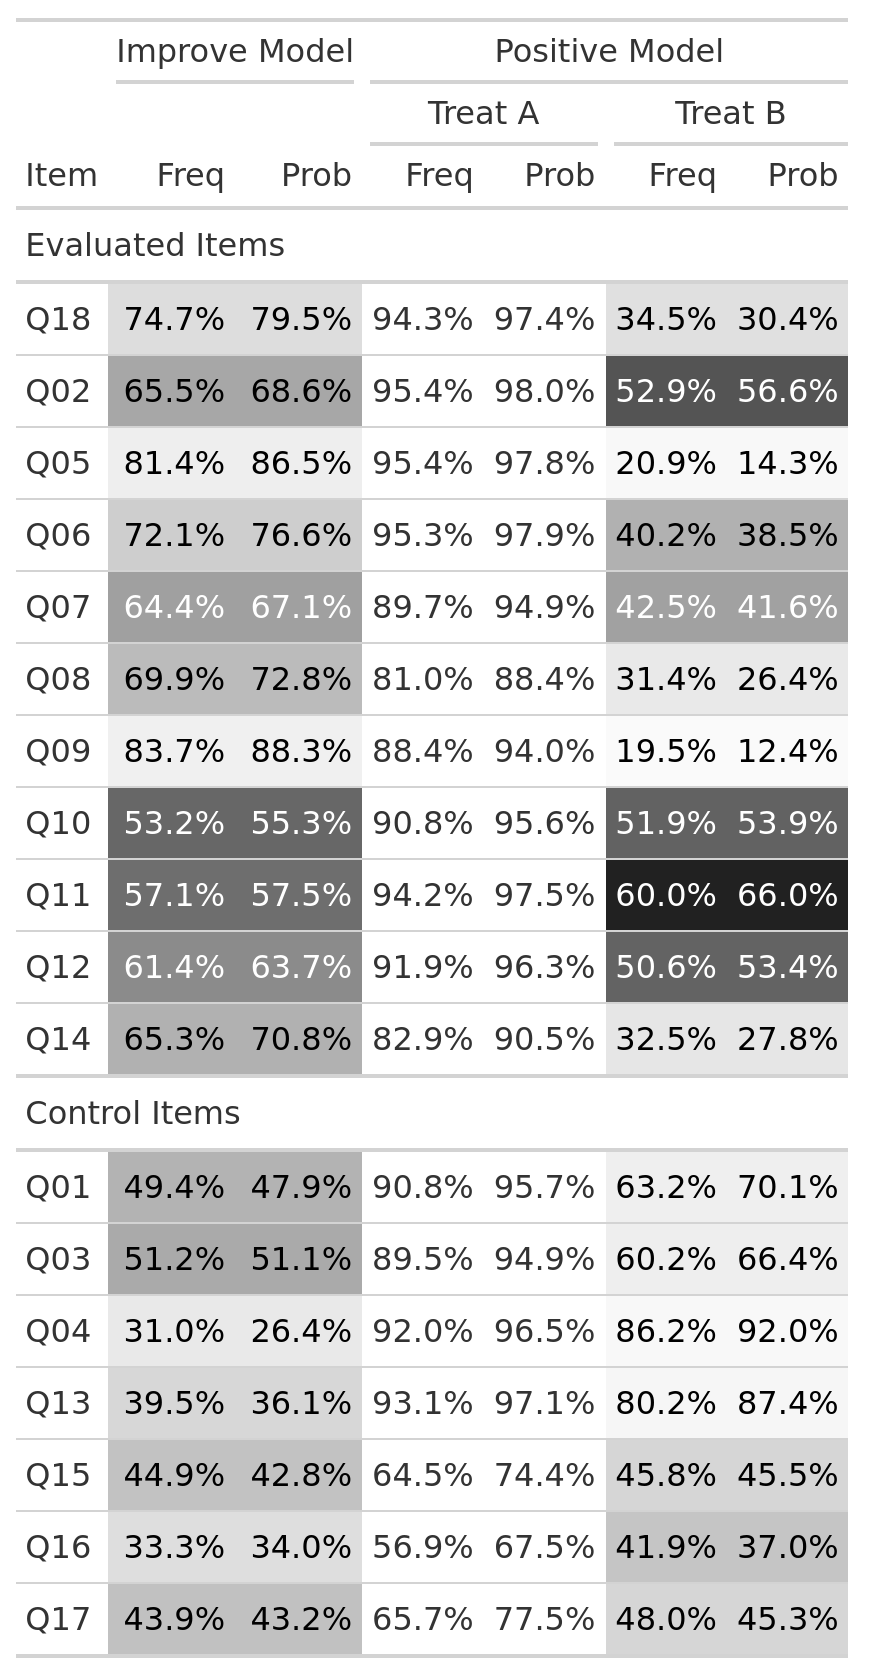
\includegraphics{images/improve.png}

}

}

\subcaption{\label{fig-or-improve}Modelo Improve (respuesta A
\textgreater{} B)}
\end{minipage}%
%
\begin{minipage}[t]{0.50\linewidth}

{\centering 

\raisebox{-\height}{

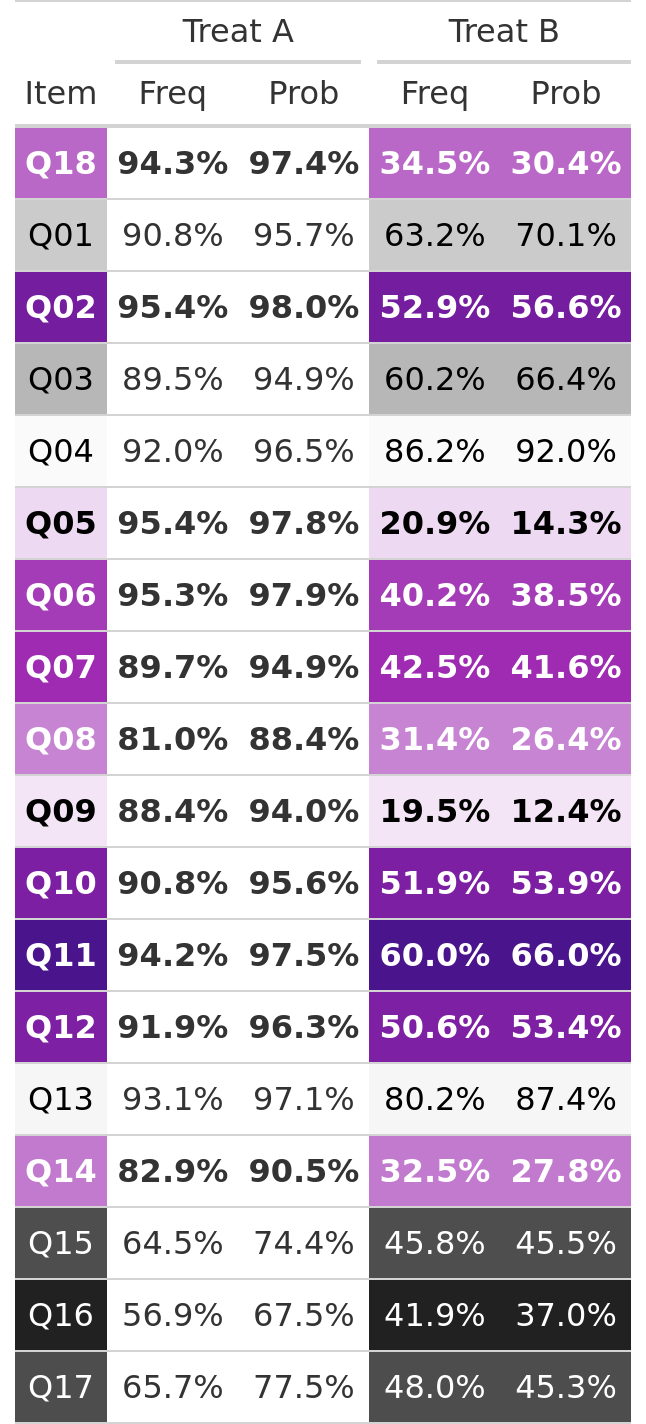
\includegraphics{images/positive.png}

}

}

\subcaption{\label{fig-or-positive}Modelo Positive (respuesta es 4 ó 5)}
\end{minipage}%

\caption{\label{fig-logistic-compare}Predicciones de los modelos de
Regresión Logística}

\end{figure}

En la Figura \ref{fig-prob-compare} se muestra la probabilidad de nivel
de respuesta por ítem y nivel de subtitulado correspondiente al modelo
de Regresión Ordinal y se compara con la frecuencia de la tabla de
contingencia. Los ítems con errores se muestran en negrita y
recuadrados. Se observa que en el subtitulado \(A\) todas las respuestas
a los ítems se concentran en valores positivos (4 ó 5). En este
subtitulado \(A\) los ítems \(Q15\), \(Q16\) y \(Q17\) reciben bastantes
respuestas negativas \footnote{El modelo ordinal no es capaz de predecir
  esto debido a que, como estos ítems recibieron muchas contestaciones
  \enquote{No sé / No contesto} y éstas se han eliminado del análisis,
  el efecto \enquote{regresión a la media} que produce el modelado en
  estos ítems es grande.}.

En el subtitulado \(B\) se espera que los ítems en los que se han
introducido errores tengan peores valoraciones. Esto sucede claramente
en \(Q05\) y en \(Q09\) y también aunque en menor medida en \(Q06\),
\(Q07\), \(Q08\) y \(Q14\). En \(Q18\) (los subtítulos del vídeo cumplen
en general con los requisitos de accesibilidad) también se observan
diferencias, lo que es una clara indicación de que los estudiantes han
considerado que \(B\) es el subtitulado con errores. Sin embargo, hay
una gran incertidumbre en las respuestas a los ítems \(Q02\), \(Q10\),
\(Q11\) y \(Q12\). En todos ellos hay más respuestas negativas que en el
subtitulado \(A\) pero se mantiene un elevado porcentaje de respuestas
positivas. En los ítems en los que no se han introducido errores se
deberían observar respuestas similares a las del subtitulado \(A\). Esto
sucede en \(Q04\), \(Q13\), \(Q15\), \(Q16\) y \(Q17\). Pero no ocurre
lo mismo en los ítems \(Q01\) y \(Q03\) ya que reciben peores
valoraciones en \(B\) que en \(A\) de forma inesperada.

Una cuestión interesante a destacar es que en general el análisis de las
predicciones del modelo ordinal es más parsimonioso y estable que el
análisis de las frecuencias relativas. Esto se va claramente en los
ítems \(Q01\), \(Q07\) y \(Q08\). El análisis en bruto de las
frecuencias muestra que las valoraciones de los estudiantes están
polarizadas y evitan la contestación neutral. El modelo ha corregido
esto y hecho unas predicciones más equilibradas.

\begin{figure}[h]
\begin{adjustwidth}{-3.4cm}{}

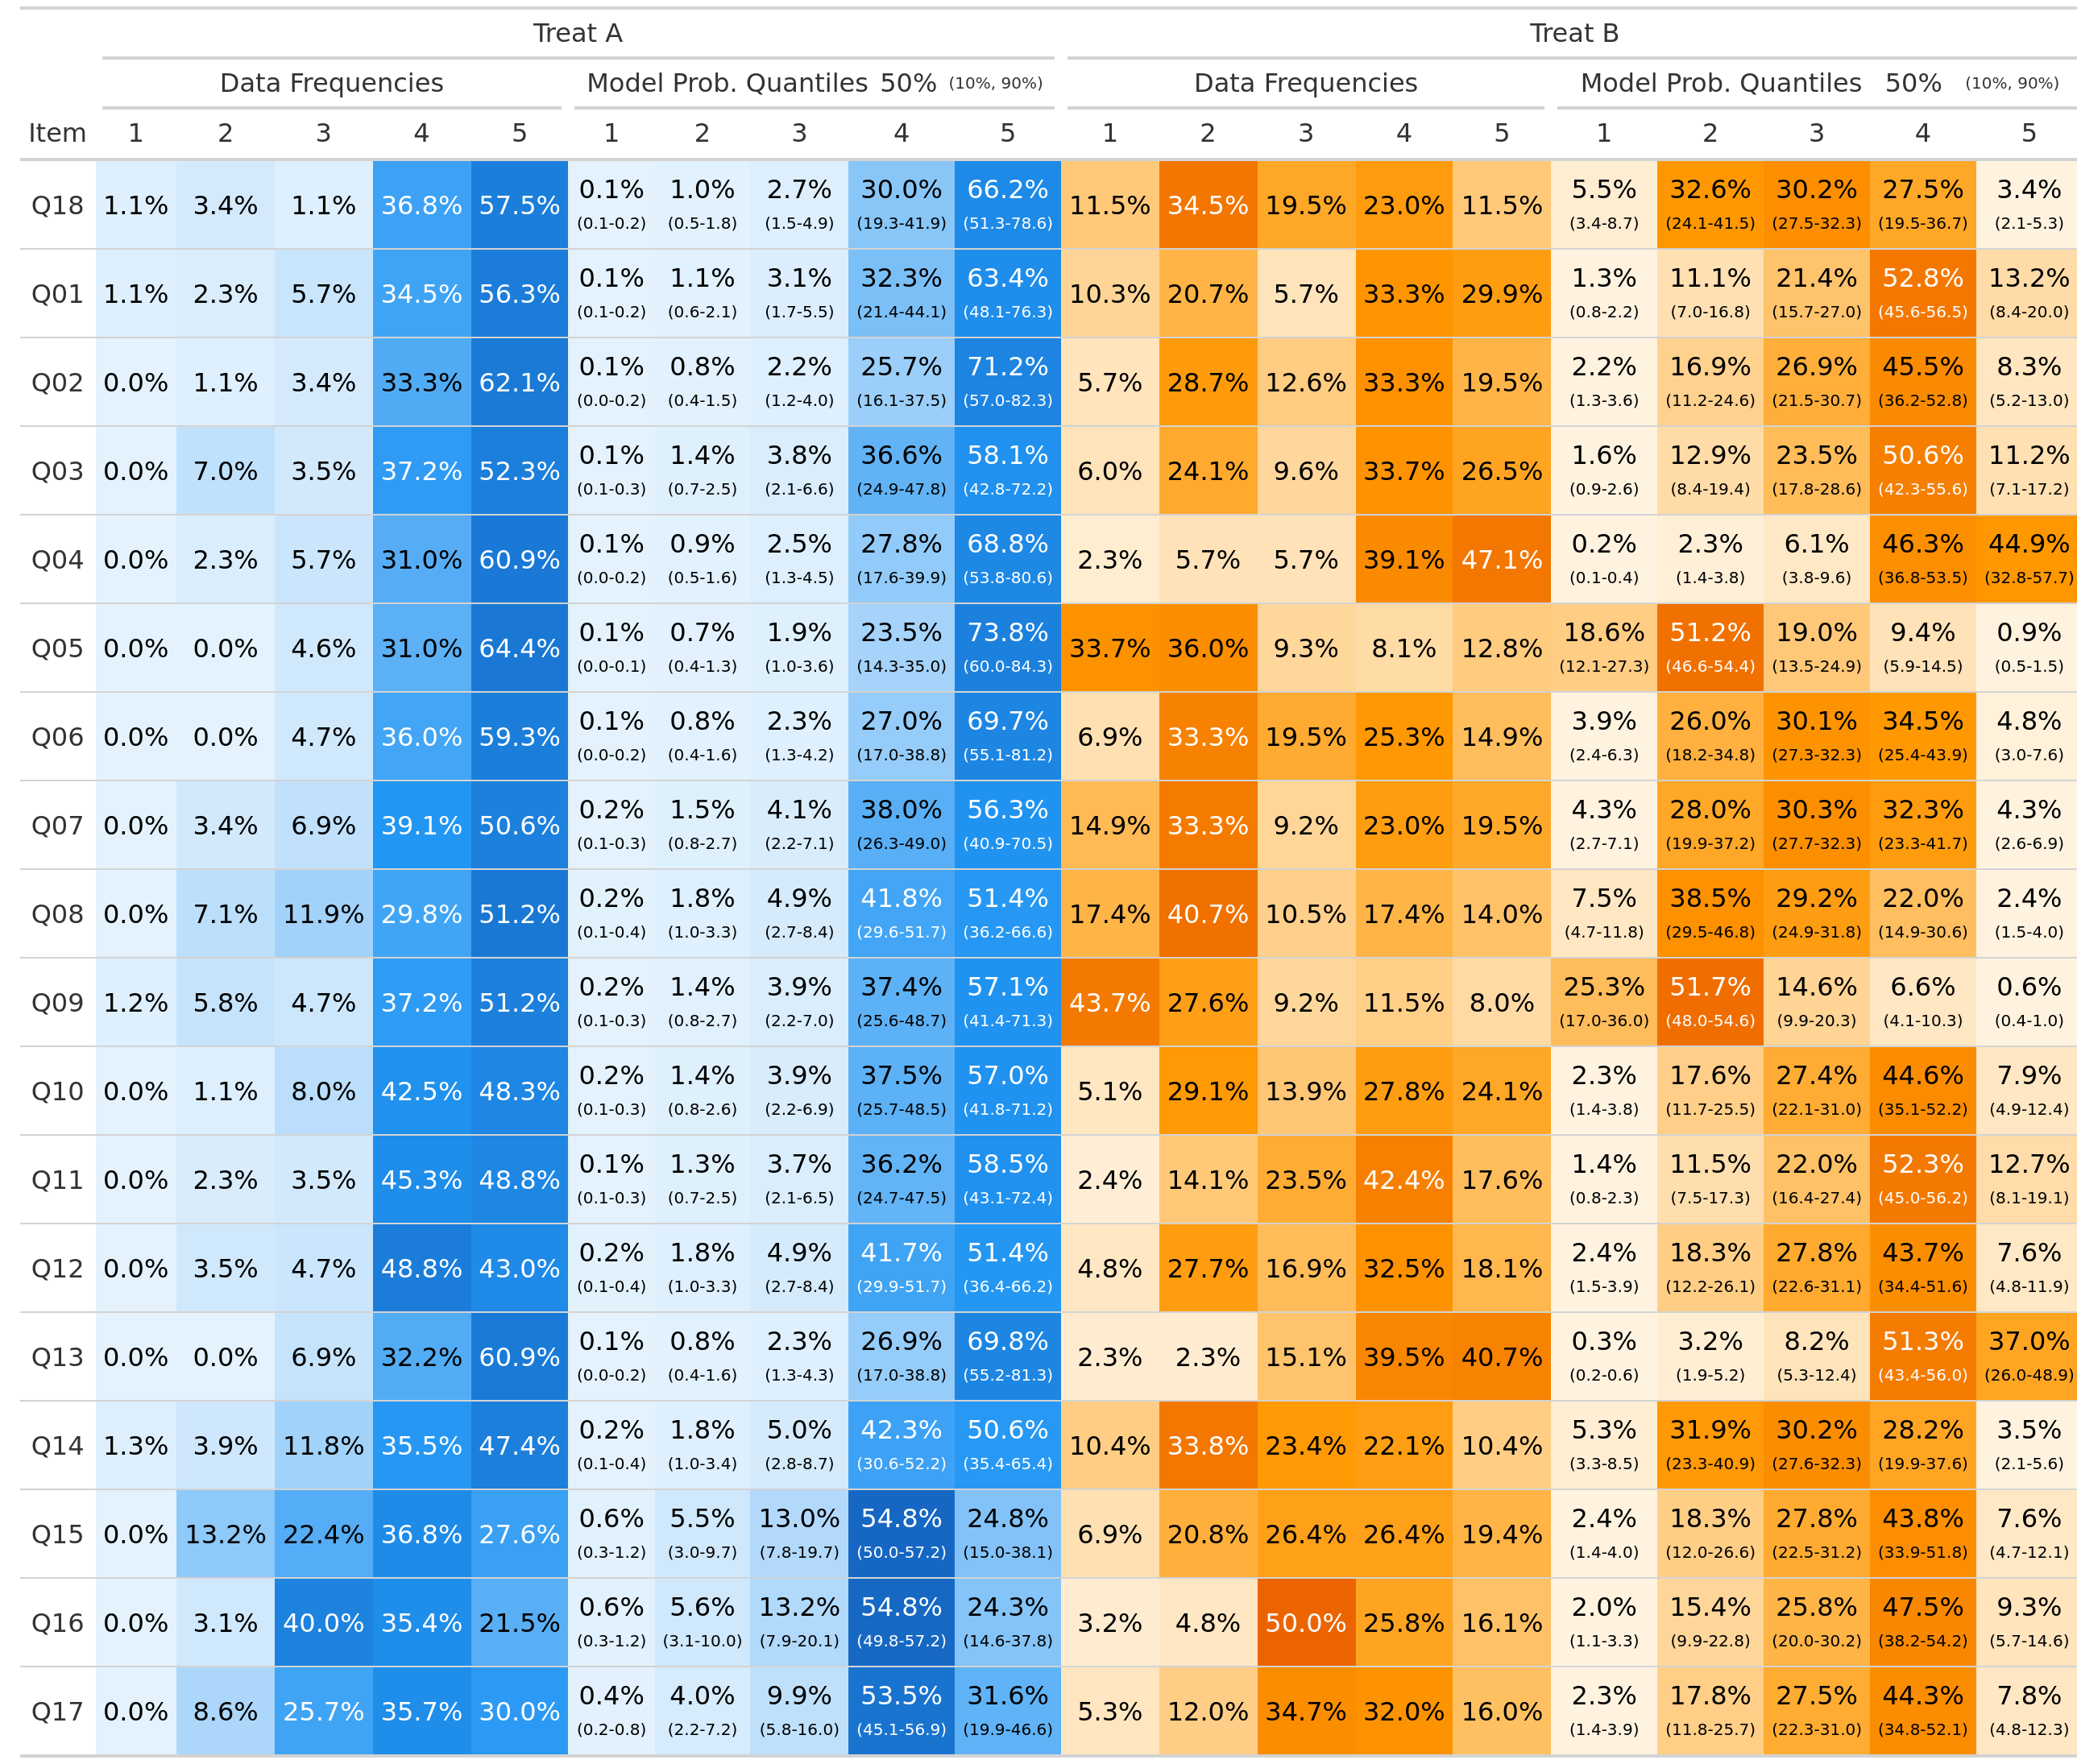
\includegraphics[width=1.2\linewidth]{images/bayes-probs.png} \hfill{}

\caption{\label{fig-prob-compare}Predicciones del modelo de Regresión Logística.}

\end{adjustwidth}
\end{figure}

Para entender las motivaciones de las valoraciones de los alumnos en
aquellos ítems que tienen una respuesta no deseada se han analizado los
comentarios que dejaron \footnote{Estos comentarios se separaron en la
  fase de preprocesado y no se han utilizado ni consultado hasta la
  realización de este capítulo.}. La siguiente es una selección de
comentarios por ítems:

\begin{itemize}
\tightlist
\item
  \(Q01\), \textbf{la posición de los subtítulos}: Se trata de un error
  no existente en ninguno de los vídeos. Sin embargo, una selección de
  comentarios (hay otros ejemplos similares) evidencia que algunos
  alumnos (pocos) han manifestado que no estaban bien posicionados los
  subtítulos en \(A\) y que otros (bastantes) han comentado que en el
  vídeo \(B\) los subtítulos no estaban bien posicionados.
\end{itemize}

\scriptsize
\color{blue}

\begin{quote}
Subtitulado \(A\) \(Q01\): \enquote*{No estaban en la parte inferior de
la pantalla}, \enquote*{en ocasiones no estan en la posicion que se
espera}. \color{black} \normalsize
\end{quote}

\scriptsize
\color{red}

\begin{quote}
Subtitulado \(B\) \(Q01\): \enquote*{Se presentaba en diferentes
posiciones}, \enquote*{cambian de sitio}, \enquote*{creo que podrian
estar un poquito mas abajo}, \enquote*{Fallos corregidos},
\enquote*{centrados}.
\end{quote}

\color{black}

\normalsize

\begin{itemize}
\tightlist
\item
  \(Q03\), \textbf{la disposición del texto respecto a la caja donde se
  muestran los subtítulos}: Se trata de un error no existente en ninguno
  de los vídeos. En los comentarios hay bastante más negativos en el
  vídeo \(A\) que en el \(B\).
\end{itemize}

\scriptsize
\color{blue}

\begin{quote}
Subtitulado \(A\) \(Q03\): \enquote*{Mejor alineado a la izquierda},
\enquote*{Palabras cortadas en los parrafos}, \enquote*{en algunos casos
no esta centrado}, \enquote*{a veces se cortan palabras y otros
detalles\ldots{}}, \enquote*{Mejor a la izquierda}, \enquote*{Centrado.
Bien}, \enquote*{Adecuado}.
\end{quote}

\color{black}
\normalsize

\begin{itemize}
\tightlist
\item
  \(Q02\), \textbf{el número de líneas por subtítulo}: Se trata de un
  error introducido en el subtitulado \(B\). En los comentarios al
  subtitulado \(A\) hay bastantes que se quejan del número excesivo de
  líneas.
\end{itemize}

\scriptsize
\color{blue}

\begin{quote}
Subtitulado \(A\) \(Q02\): \enquote*{Se pueden hasta 3 pero no es
recomendable}, \enquote*{en ocasiones son 3 innecesariamente},
\enquote*{frases muy cortas}, \enquote*{No superaba las dos (creo
recordar)}, \enquote*{Se cumple}.
\end{quote}

\color{black}
\normalsize

\begin{itemize}
\tightlist
\item
  \(Q10\), \textbf{la sincronización de las entradas y salidas de los
  subtítulos}: Se trata de un error introducido en el subtitulado \(B\).
  En los comentarios al subtitulado \(A\) hay algunos que dicen que hay
  falta de sincronización y, por el contrario, en el \(B\) que estaban
  bien sincronizados. Hay por tanto una falta de atención de algunos
  estudiantes para evaluar este aspecto del subtitulado.
\end{itemize}

\scriptsize
\color{blue}

\begin{quote}
Subtitulado \(A\) \(Q10\): \enquote*{Van a destiempo}, \enquote*{a veces
hay retardo del texto sobre el audio}, \enquote*{No me dado cuenta.},
\enquote*{Estaban desincronizadas}.
\end{quote}

\color{black}
\normalsize

\scriptsize
\color{red}

\begin{quote}
Subtitulado \(B\) \(Q10\): \enquote*{Regular.}, \enquote*{Sincronizado},
\enquote*{bastante sincronizados}, \enquote*{va a la paz texto y
lenguaje}, \enquote*{Estaba bien sincronizado}, \enquote*{Fallos
corregidos}, \enquote*{sincronizadas con el audio y la imagen}.
\end{quote}

\color{black}
\normalsize

\begin{itemize}
\tightlist
\item
  \(Q11\), \textbf{la velocidad de exposición de los subtítulos}: Se
  trata de un error introducido en el subtitulado \(B\). Los comentarios
  al subtitulado \(B\) denotan que muchos estudiantes no han tenido en
  cuenta el subtítulo debe permanecer al menos tres segundos en la
  pantalla.
\end{itemize}

\scriptsize
\color{red}

\begin{quote}
Subtitulado \(B\) \(Q11\): \enquote*{Sincronizado.}, \enquote*{me ha
parecido un tiempo suficiente}, \enquote*{los pude leer bien},
\enquote*{Buen tiempo para la lectura}, \enquote*{Se corresponde con los
12 caracteres por segundo}, \enquote*{velocidad apropiada},
\enquote*{Velocidad adequada para una buena lectura}.
\end{quote}

\color{black}
\normalsize

\begin{itemize}
\tightlist
\item
  \(Q12\), \textbf{el máximo número de caracteres por línea}: Se trata
  de un error introducido en el subtitulado \(B\). Los comentarios
  denotan que en general los alumnos conocen el número máximo de
  caracteres por línea, pero que no se han detenido a medir cuántos hay
  realmente.
\end{itemize}

\scriptsize
\color{blue}

\begin{quote}
Subtitulado \(A\) \(Q12\): \enquote*{No sobrepasa los 40 caracteres}.
\end{quote}

\color{black}
\normalsize

\scriptsize
\color{red}

\begin{quote}
Subtitulado \(B\) \(Q12\): \enquote*{No pasa de 37}, \enquote*{Se
encuentran entre 12 y 37}.
\end{quote}

\color{black}
\normalsize

\begin{itemize}
\tightlist
\item
  \(Q15\), \textbf{la utilización de puntos suspensivos}: En este ítem
  no se han introducido diferencias entre subtitulados. Aquí parece que
  los comentarios reflejan que el estudiante conoce las normas del uso
  de puntos suspensivos pero no ha prestado atención a su utilización.
  También se observan diferencias en las respuestas a la hora de valorar
  un ítem del que no tienen recuerdo, dándose todo tipo de situaciones:
  Contestar \enquote{No sé / No contesto}, contestar \enquote{Neutral} e
  incluso valorar positiva y negativamente.
\end{itemize}

\scriptsize
\color{blue}

\begin{quote}
Subtitulado \(A\) \(Q15\): \enquote*{Uso inadecuado de los puntos
suspensivos}, \enquote*{No lo recuerdo}, \enquote*{No me he fijado si
los tiene}, \enquote*{No recuerdo}, \enquote*{igual}.
\end{quote}

\color{black}
\normalsize

\scriptsize
\color{red}

\begin{quote}
Subtitulado \(B\) \(Q15\): \enquote*{solo he visto en una frase},
\enquote*{Creo que cumple con las reglas gramaticales.}, \enquote*{No
parece abusar de los puntos suspensivos}, \enquote*{Si se precisan, se
deben poner}, \enquote*{No parece usar mucho los puntos suspensivos},
\enquote*{Buen uso de los puntos supensivos}.
\end{quote}

\color{black}
\normalsize

\begin{itemize}
\tightlist
\item
  \(Q16\), \textbf{la escritura de los números}: En este ítem no se han
  introducido diferencias entre subtitulados. Tiene comparativamente
  menos comentarios que otros ítems y la mayoría reflejan que no había
  números en los subtítulos. La dispersión en las respuestas se debe,
  como en el caso de \(Q15\), a que los estudiantes no saben qué valor
  de respuesta otorgar.
\end{itemize}

\scriptsize
\color{blue}

\begin{quote}
Subtitulado \(A\) \(Q16\): \enquote*{No lo recuerdo}, \enquote*{NO
recuerdo}, \enquote*{no hay}, \enquote*{no hay}.
\end{quote}

\color{black}
\normalsize

\scriptsize
\color{red}

\begin{quote}
Subtitulado \(B\) \(Q16\): \enquote*{creo que no hay}, \enquote*{No los
he visto}, \enquote*{No lo he apreciado}.
\end{quote}

\color{black}
\normalsize

\begin{itemize}
\tightlist
\item
  \(Q17\), \textbf{las incorrecciones en el habla}: En este ítem no se
  han introducido diferencias entre subtitulados. Nuevamente los
  estudiantes detectan que no hay incorrecciones en el subtitulado pero
  no dan el mismo nivel de respuesta a esta circunstancia.
\end{itemize}

\scriptsize
\color{blue}

\begin{quote}
Subtitulado \(A\) \(Q17\): \enquote*{No he visto}, \enquote*{No he visto
ninguna}, \enquote*{No me ha parecido encontrarlas}, \enquote*{no las he
visto}, \enquote*{No las he visto}, \enquote*{Si lo lleva en el
original}.
\end{quote}

\color{black}
\normalsize

\scriptsize
\color{red}

\begin{quote}
Subtitulado \(B\) \(Q17\): \enquote*{No observp}, \enquote*{No lo he
apreciado}, \enquote*{no recuerdo incorrecciones}, \enquote*{No aparecen
incorrecciones, o al menos no las he detectado.}, \enquote*{No hay
incorrecciones en el video}.
\end{quote}

\color{black}
\normalsize

\bookmarksetup{startatroot}

\hypertarget{sec-conclusion}{%
\chapter{Conclusión y trabajo futuro}\label{sec-conclusion}}

Este trabajo ha prentendido responder a la pregunta de investigación de
si los estudiantes de un curso de \gls{accesibilidad} son capaces de
identificar los errores en el subtitulado de un vídeo, y como objetivos
específicos averiguar qué aspectos del subtitulado han sido más
fácilmente reconocidos por los estudiantes y en cuáles han tenido más
dificultad. Para ello se ha partido de una Exploración Inicial (ver
Sección~\ref{sec-eda}) y se han propuesto varios modelos estadísticos
que tengan en cuenta la naturaleza ordinal y dependiente de la variable
respuesta (ver Sección~\ref{sec-modelos-utilizados}). Como variables
explicativas se ha considerado el nivel de subtitulado, el periodo en el
que se ha realizado cada test, la secuencia u orden de realización de
los test, el estudiante que ha realizado el test y el ítem al que se
responde.

La conclusión más importante es que todos los análisis estadísticos
realizados muestran que el nivel de subtitulado es la variable que mejor
explica la respuesta a cada ítem. Los efectos secuencia y periodo son
comparativamente de poca importancia y se traducen en que en general los
estudiantes valoran peor el vídeo visto en el segundo periodo para un
mismo nivel de subtitulado. Las variables estudiante e ítem se han
tratado como efectos aleatorios por haber considerado que sus
observaciones no son independientes. La varianza explicada por la
variable estudiante ha sido más grande que la explicada por la variable
ítem.

Los estudiantes han sabido reconocer los errores de subtitulado de los
ítems \(Q05\) (la corrección ortográfica y gramatical), \(Q06\) (la
literalidad), \(Q07\) (la identificación de los personajes), \(Q08\) (la
asignación de líneas a los personajes en los diálogos), \(Q09\) (la
descripción de efectos sonoros) y \(Q14\) (la separación en líneas
diferentes de sintagmas nominales, verbales y preposicionales).

Sin embargo, han tenido más dificultades en indentificar los errores
introducidos en los ítems \(Q02\) (el número de líneas por subtítulo),
\(Q10\) (la sincronización de las entradas y salidas de los subtítulos),
\(Q11\) (la velocidad de exposición de los subtítulos) y \(Q12\) (el
máximo número de caracteres por línea). El análisis realizado sobre los
comentarios a estos ítems, evidencia que los estudiantes han aprendido
las normas que debe regir el subtitulado en estos aspectos pero que no
han evaluado minuciosamente si se cumplen realmente. Hay que tener en
consideración que esta fue una actividad voluntaria sin incidencia en la
calificación del curso, y que en una situación real esto no habría
sucedido y habrían realizado una corroboración minuciosa.

En definitiva, los estudiantes conocen las normas de subtitulado y son
capaces identificar los errores que no requieren una comprobación
exhaustiva. En los que sí lo requieren, algunos estudiantes han
contestado sin realizar las comprobaciones necesarias.

En cuanto a los ítems que tratan aspectos en los que no hay errores en
ninguno de los vídeos, los estudiantes han valorado positivamente ambos
subtitulados en los ítems \(Q04\) (el contraste entre los caracteres y
el fondo) y \(Q13\) (la legibilidad de la tipografía). Esto no implica
necesariamente que, de haber habido deficiencias en estos aspectos, las
hubieran reconocido. De hecho, hay evidencias de que los estudiantes
noveles tienen dificultades en la identificación de deficiencias en el
contraste \autocite[ver][]{jperez2}.

En los ítems \(Q01\) (la posición de los subtítulos) y \(Q03\) (la
disposición del texto respecto a la caja donde se muestran los
subtítulos) los alumnos han manifestado en los comentarios la existencia
de problemas en el ítem \(Q01\) en el subtitulado \(B\) y en el ítem
\(Q03\) y subtitulado \(A\). Sería conveniente que fuera evaluado por un
experto en subtitulado si realmente los subtítulos son correctos en
estos aspectos o si es que no han sido evaluados adecuadamente por los
estudiantes.

Los ítems \(Q15\) (la utilización de puntos suspensivos), \(Q16\) (la
escritura de los números) y \(Q17\) (las incorrecciones en el habla)
preguntan cuestiones que no se producen en los vídeos y que son
relativamente fáciles de verificar. En las respuestas de los estudiantes
han confluido varios problemas verificables a través de los comentarios
a los ítems. Por un lado, algunos estudiantes manifiestan que no
recuerdan con seguridad la existencia de lo preguntado (puntos
suspensivos, números, \ldots). Este problema no es importante ya que es
de suponer que en una situación de evaluación de subtitulado real
realizarían un segundo visionado de los vídeos para asegurarse. Más
preocupante resulta el segundo de los problemas detectados ya que podría
estar también presente en otros ítems y haber pasado invadvertido en
este trabajo. El problema en cuestión es que en estos ítems la respuesta
esperable es \enquote{No sé / No contesto}. En la
Tabla~\ref{tbl-no-response} se constató que estos son los ítems que más
respuestas de este nivel reciben pero que esta respuesta no es masiva.
Muchos estudiantes se decantan por valoraciones negativas, positivas o
neutrales a pesar de haber indicado en los comentrios que la pregunta
realizada no tiene aplicación en la actividad. Este problema es una
preocupación general en análisis de escalas de Likert. Por ejemplo, ver
\textcite{tutz2020} para una propuesta de modelado estadístico de la
categoría neutral en una escala de Likert. Un tercer problema detectado
en estos ítems que es probable que también haya tenido incidencia en
otros ítems es que, a pesar de que los comentarios revelan que los
estudiantes piensan que estos ítems no tienen aplicación en ninguno de
los vídeos, obtienen peor valoración en el subtitulado \(B\) que en el
\(A\). Esto estaría indicando que las contestaciones de los estudiantes
sufren cierto \enquote{efecto de ventana rota}. La hipótesis que aquí se
plantea para explicar por qué el subtitulado \(B\) ha obtenido peores
respuestas que el \(A\) incluso en ítems en los que el estudiante sabe
que los subtitulados son idénticos es la siguiente: Hay ítems como
\(Q05\) (la corrección ortográfica y gramatical) que son fáciles de
identificar y responder por los estudiantes. Si el estudiante encuentra
una falta de ortografía en un subtitulado, estaría psicológicamente
condicionado a ser más crítico con cualquier otro aspecto del
subtitulado. Ante una pregunta que el estudiante no recuerda haber
encontrado (por ejemplo, la presencia de puntos suspensivos) tiene a una
valoración inferior en el subtitulado con faltas de ortografía porque
considera que existe la posibilidad de haber pasado por alto la
presencia de puntos suspensivos. Esto no sucede en todos los casos. Por
ejemplo, en la pregunta sobre el contraste (ítem \(Q04\)), la diferencia
entre subtitulados aunque existe es menor. La hipótesis expuesta es
coherente con este hecho ya que, mientras que los puntos suspensivos son
algo puntual cuya existencia el estudiante sabe que puede pasar
inadvertida, el contraste es algo que afecta o puede afectar a todo el
subtitulado del vídeo.

Estas conclusiones abren varias vías de investigación que se enumeran
aquí a modo de propuesta y sin ánimo de exhaustividad:

\begin{itemize}
\tightlist
\item
  Incorporar al modelo variables como el sexo, la edad, el lugar de
  nacimiento, el nivel de estudios o el grado de conocimientos de
  accesibilidad previo. En el momento de realizar este trabajo se
  disponía de esta información aunque de forma muy incompleta ya que la
  mayoría de los estudiantes participantes no suministraron la
  información personal.
\item
  Volver a realizar el análisis completo con los mismos datos pero
  incorporando desde el principio el conocimiento del subtitulado
  correcto y siendo más crítico con la calidad de los datos, lo que
  llevaría a eliminar alguno de los cuestiorarios.
\item
  Analizar los datos de la edición del curso de 2023 para ver en qué
  medida los modelos y las conclusiones se mantienen o cambian.
\item
  Plantear mejoras en la recogida de datos como, por ejemplo,
  indicaciones detalladas de como responder en caso de duda,
  desconocimiento, inaplicabilidad, \ldots.
\item
  Sería interesante ver cómo cambian las respuestas de los estudiantes
  si en ambos vídeos se introducen errores en el subtitulado en
  diferentes aspectos.
\item
  Añadir errores de subtitulado para todos o casi todos los ítems.
\item
  Además de las respuestas de los estudiantes, se podría plantear la
  actividad a profesionales del subtitulado para evaluar las semejanzas
  y diferencias entre grupos.
\end{itemize}

\cleardoublepage
\phantomsection
\addcontentsline{toc}{part}{Apéndices}
\appendix

\hypertarget{sec-contrasts}{%
\chapter{Efecto secuencia e interacción tratamiento
vs.~periodo}\label{sec-contrasts}}

Se va a demostrar que el \gls{efecto secuencia} es equivalente a la
interacción de los factores tratamiento y periodo.

\hypertarget{preparaciuxf3n}{%
\section{Preparación}\label{preparaciuxf3n}}

Partiendo del siguiente conjunto de datos generado aleatoriamente
\footnote{Obsérvese que la variable \texttt{Response} en esta simulación
  es cuantitativa y no ordinal. Se ha realizado de esta forma para poder
  usar un ajuste de mínimos cuadrados en lugar de una regresión ordinal
  para facilitar el cálculo y su interpretación.}: \scriptsize

\begin{Shaded}
\begin{Highlighting}[]
\FunctionTok{set.seed}\NormalTok{(}\DecValTok{100}\NormalTok{)}
\NormalTok{n }\OtherTok{\textless{}{-}} \DecValTok{1000}
\NormalTok{df }\OtherTok{\textless{}{-}} \FunctionTok{data.frame}\NormalTok{(}
    \AttributeTok{Response =} \FunctionTok{rnorm}\NormalTok{(n),}
    \AttributeTok{Treat =} \FunctionTok{as.factor}\NormalTok{(}\FunctionTok{sample}\NormalTok{(}\FunctionTok{c}\NormalTok{(}\StringTok{"A"}\NormalTok{, }\StringTok{"B"}\NormalTok{), n, }\AttributeTok{replace =} \ConstantTok{TRUE}\NormalTok{)),}
    \AttributeTok{Period =} \FunctionTok{as.factor}\NormalTok{(}\FunctionTok{sample}\NormalTok{(}\FunctionTok{c}\NormalTok{(}\DecValTok{1}\NormalTok{, }\DecValTok{2}\NormalTok{), n, }\AttributeTok{replace =} \ConstantTok{TRUE}\NormalTok{))}
\NormalTok{)}

\NormalTok{df}\SpecialCharTok{$}\NormalTok{Seq }\OtherTok{\textless{}{-}} \FunctionTok{as.factor}\NormalTok{(}
    \FunctionTok{ifelse}\NormalTok{(}
\NormalTok{        df}\SpecialCharTok{$}\NormalTok{Period }\SpecialCharTok{==} \DecValTok{1} \SpecialCharTok{\&}\NormalTok{ df}\SpecialCharTok{$}\NormalTok{Treat }\SpecialCharTok{==} \StringTok{"A"} \SpecialCharTok{|}\NormalTok{ df}\SpecialCharTok{$}\NormalTok{Period }\SpecialCharTok{==} \DecValTok{2} \SpecialCharTok{\&}\NormalTok{ df}\SpecialCharTok{$}\NormalTok{Treat }\SpecialCharTok{==} \StringTok{"B"}\NormalTok{,}
        \StringTok{"AB"}\NormalTok{,}
        \StringTok{"BA"}
\NormalTok{    )}
\NormalTok{)}

\FunctionTok{head}\NormalTok{(df, }\DecValTok{10}\NormalTok{)}
\end{Highlighting}
\end{Shaded}

\begin{verbatim}
      Response Treat Period Seq
1  -0.50219235     B      2  AB
2   0.13153117     A      1  AB
3  -0.07891709     A      2  BA
4   0.88678481     A      2  BA
5   0.11697127     A      1  AB
6   0.31863009     A      2  BA
7  -0.58179068     A      2  BA
8   0.71453271     A      1  AB
9  -0.82525943     B      2  AB
10 -0.35986213     B      1  BA
\end{verbatim}

\normalsize

Se calculan las medias por cada nivel de factor y combinaciones de
niveles que luego serán utilizadas en la interpretación de los
coeficientes de los modelos:

\scriptsize

\begin{Shaded}
\begin{Highlighting}[]
\NormalTok{M }\OtherTok{\textless{}{-}} \FunctionTok{mean}\NormalTok{(df}\SpecialCharTok{$}\NormalTok{Response) }\CommentTok{\# 1 media de respuesta global}

\CommentTok{\# 2 medias de respuesta para tratamientos A y B}
\NormalTok{mTreat }\OtherTok{\textless{}{-}} \FunctionTok{with}\NormalTok{(df, }\FunctionTok{tapply}\NormalTok{(Response, Treat, mean))}

\CommentTok{\# 2 medias de respuesta para periodos 1 y 2}
\NormalTok{mPeriod }\OtherTok{\textless{}{-}} \FunctionTok{with}\NormalTok{(df, }\FunctionTok{tapply}\NormalTok{(Response, Period, mean))}

\CommentTok{\# 2 medias de respuesta para secuencias AB y BA}
\NormalTok{mSeq }\OtherTok{\textless{}{-}} \FunctionTok{with}\NormalTok{(df, }\FunctionTok{tapply}\NormalTok{(Response, Seq, mean))}

\CommentTok{\# 4 medias de respuesta para las cuatro combinaciones de tratamiento y periodo}
\NormalTok{m2 }\OtherTok{\textless{}{-}} \FunctionTok{with}\NormalTok{(df, }\FunctionTok{tapply}\NormalTok{(Response, }\FunctionTok{list}\NormalTok{(Treat, Period), mean))}

\NormalTok{dTreat }\OtherTok{\textless{}{-}} \FunctionTok{diff}\NormalTok{(mTreat) }\CommentTok{\# diferencia de medias entre tratamientos A y B}

\NormalTok{dPeriod }\OtherTok{\textless{}{-}} \FunctionTok{diff}\NormalTok{(mPeriod) }\CommentTok{\# diferencia de medias entre periodos 1 y 2}

\NormalTok{d2 }\OtherTok{\textless{}{-}} \FunctionTok{diff}\NormalTok{(m2) }\CommentTok{\# diferencias entre niveles de tratamiento en cada nivel de periodo}
\end{Highlighting}
\end{Shaded}

\normalsize

\hypertarget{anuxe1lisis-con-un-solo-factor-tratamiento}{%
\section{Análisis con un solo factor
(tratamiento)}\label{anuxe1lisis-con-un-solo-factor-tratamiento}}

\scriptsize

\begin{Shaded}
\begin{Highlighting}[]
\NormalTok{l1 }\OtherTok{\textless{}{-}} \FunctionTok{lm}\NormalTok{(Response }\SpecialCharTok{\textasciitilde{}}\NormalTok{ Treat, df)}
\FunctionTok{data.frame}\NormalTok{(}\FunctionTok{t}\NormalTok{(}\FunctionTok{coef}\NormalTok{(l1))) }\SpecialCharTok{\%\textgreater{}\%} \FunctionTok{gt}\NormalTok{()}
\end{Highlighting}
\end{Shaded}

\hypertarget{tbl-l1}{}
\begin{longtable}{rr}
\caption{\label{tbl-l1}Ajuste del modelo Response \textasciitilde{} Treat con contrasts
treatment. }\tabularnewline

\toprule
X.Intercept. & TreatB \\ 
\midrule
0.03624217 & -0.03966751 \\ 
\bottomrule
\end{longtable}

\normalsize

Se comprueba que el intercepto es la media de la respuesta en el nivel
de tratamiento \(A\):

\scriptsize

\begin{Shaded}
\begin{Highlighting}[]
\NormalTok{mTreat[}\DecValTok{1}\NormalTok{]}
\end{Highlighting}
\end{Shaded}

\begin{verbatim}
         A 
0.03624217 
\end{verbatim}

\normalsize

Que la pendiente (parámetro \(TreatB\)) es la diferencia entre las
medias tratamientos:

\scriptsize

\begin{Shaded}
\begin{Highlighting}[]
\NormalTok{dTreat}
\end{Highlighting}
\end{Shaded}

\begin{verbatim}
          B 
-0.03966751 
\end{verbatim}

\normalsize

Por ello, para conocer el efecto del tratamiento en el nivel \(B\) hay
que sumar intercepto y pendiente:

\scriptsize

\begin{Shaded}
\begin{Highlighting}[]
\FunctionTok{coef}\NormalTok{(l1)[[}\DecValTok{1}\NormalTok{]] }\SpecialCharTok{+} \FunctionTok{coef}\NormalTok{(l1)[[}\DecValTok{2}\NormalTok{]] }\SpecialCharTok{{-}}\NormalTok{ mTreat[[}\DecValTok{2}\NormalTok{]]}
\end{Highlighting}
\end{Shaded}

\begin{verbatim}
[1] 1.214306e-16
\end{verbatim}

\normalsize

Esto es así ya que por defecto R utiliza el contraste conocido como
\texttt{codificación\ de\ tratamiento}:

\scriptsize

\begin{Shaded}
\begin{Highlighting}[]
\FunctionTok{contr.treatment}\NormalTok{(}\DecValTok{2}\NormalTok{)}
\end{Highlighting}
\end{Shaded}

\begin{verbatim}
  2
1 0
2 1
\end{verbatim}

\normalsize

La matriz ampliada añadiendo el intercepto siempre tendrá una columna de
1's:

\scriptsize

\begin{Shaded}
\begin{Highlighting}[]
\FunctionTok{model.matrix}\NormalTok{(}\SpecialCharTok{\textasciitilde{}}\NormalTok{Treat, }\FunctionTok{expand.grid}\NormalTok{(}\AttributeTok{Treat =} \FunctionTok{c}\NormalTok{(}\StringTok{"A"}\NormalTok{, }\StringTok{"B"}\NormalTok{)))}
\end{Highlighting}
\end{Shaded}

\begin{verbatim}
  (Intercept) TreatB
1           1      0
2           1      1
attr(,"assign")
[1] 0 1
attr(,"contrasts")
attr(,"contrasts")$Treat
[1] "contr.treatment"
\end{verbatim}

\normalsize

Cada fila representa el nivel del tratamiento (fila 1 nivel \(A\) y fila
2 nivel \(B\)) y las columnas representan los parámetros del modelo. Los
valores son los niveles de tratamiento (0 ó 1). Para obtener el
significado de cada parámetro, se multiplica el valor del contraste por
el parámetro. Así:

\begin{itemize}
\tightlist
\item
  En la primera fila se comprueba que el efecto del tratamiento \(A\) es
  el intercepto: \(A = 1 \cdot Intercept + 0 \cdot TreatB\).
\item
  En la segunda fila permite comprobar que el valor del parámetro
  \(TreatB\) es la diferencia de los niveles de tratamiento.
  \(B = 1 \cdot Intercept + 1 \cdot TreatB \Rightarrow TreatB = B - Intercept\).
\end{itemize}

Esto quiere decir que existe una variable para codificar el efecto
tratamiento, y esta variable tiene el valor 0 para el nivel \(A\) por
ser el de referencia y 1 para el nivel \(B\). La pendiente se codifica
como la diferencia del efecto de los dos niveles (\(B - A\)).

\hypertarget{anuxe1lisis-con-un-dos-factores-tratamiento-y-periodo}{%
\section{Análisis con un dos factores (tratamiento y
periodo)}\label{anuxe1lisis-con-un-dos-factores-tratamiento-y-periodo}}

\scriptsize

\begin{Shaded}
\begin{Highlighting}[]
\NormalTok{l2 }\OtherTok{\textless{}{-}} \FunctionTok{lm}\NormalTok{(Response }\SpecialCharTok{\textasciitilde{}}\NormalTok{ Treat }\SpecialCharTok{*}\NormalTok{ Period, df)}
\FunctionTok{data.frame}\NormalTok{(}\FunctionTok{t}\NormalTok{(}\FunctionTok{coef}\NormalTok{(l2))) }\SpecialCharTok{\%\textgreater{}\%} \FunctionTok{gt}\NormalTok{()}
\end{Highlighting}
\end{Shaded}

\hypertarget{tbl-l2}{}
\begin{longtable}{rrrr}
\caption{\label{tbl-l2}Ajuste del modelo Response \textasciitilde{} Treat * Period con
contrasts treatment. }\tabularnewline

\toprule
X.Intercept. & TreatB & Period2 & TreatB.Period2 \\ 
\midrule
0.04138614 & -0.1076137 & -0.01125933 & 0.1343517 \\ 
\bottomrule
\end{longtable}

\normalsize

Se comprueba que el intercepto es la media del tratamiento \(A\) en el
periodo \(1\) por ser estos los valores que R usa como referencia
\footnote{R utiliza como valor de referencia el nivel más bajo de
  factor.}:

\scriptsize

\begin{Shaded}
\begin{Highlighting}[]
\NormalTok{m2[}\StringTok{"A"}\NormalTok{, }\StringTok{"1"}\NormalTok{]}
\end{Highlighting}
\end{Shaded}

\begin{verbatim}
[1] 0.04138614
\end{verbatim}

\normalsize

El parámetro \(TreatB\) es la diferencia de medias entre los
tratamientos en el periodo \(1\):

\scriptsize

\begin{Shaded}
\begin{Highlighting}[]
\NormalTok{m2[}\StringTok{"B"}\NormalTok{, }\StringTok{"1"}\NormalTok{] }\SpecialCharTok{{-}}\NormalTok{ m2[}\StringTok{"A"}\NormalTok{, }\StringTok{"1"}\NormalTok{]}
\end{Highlighting}
\end{Shaded}

\begin{verbatim}
[1] -0.1076137
\end{verbatim}

\normalsize

El parámetro \(Period2\) es la diferencia de medias entre los periodos
en el nivel de tratamiento \(A\):

\scriptsize

\begin{Shaded}
\begin{Highlighting}[]
\NormalTok{m2[}\StringTok{"A"}\NormalTok{, }\StringTok{"2"}\NormalTok{] }\SpecialCharTok{{-}}\NormalTok{ m2[}\StringTok{"A"}\NormalTok{, }\StringTok{"1"}\NormalTok{]}
\end{Highlighting}
\end{Shaded}

\begin{verbatim}
[1] -0.01125933
\end{verbatim}

\normalsize

Finalmente, \(TreatB:Period2\) es la diferencia entre el segundo periodo
y el primero del nivel de tratamiento \(B\) menos la diferencia entre
periodos del nivel de tratamiento \(A\):

\scriptsize

\begin{Shaded}
\begin{Highlighting}[]
\NormalTok{m2[}\StringTok{"B"}\NormalTok{, }\StringTok{"2"}\NormalTok{] }\SpecialCharTok{{-}}\NormalTok{ m2[}\StringTok{"B"}\NormalTok{, }\StringTok{"1"}\NormalTok{] }\SpecialCharTok{{-}}\NormalTok{ (m2[}\StringTok{"A"}\NormalTok{, }\StringTok{"2"}\NormalTok{] }\SpecialCharTok{{-}}\NormalTok{ m2[}\StringTok{"A"}\NormalTok{, }\StringTok{"1"}\NormalTok{])}
\end{Highlighting}
\end{Shaded}

\begin{verbatim}
[1] 0.1343517
\end{verbatim}

\normalsize

La matriz de contraste nos permite razonar por qué esto es así:

\scriptsize

\begin{Shaded}
\begin{Highlighting}[]
\FunctionTok{model.matrix}\NormalTok{(}\SpecialCharTok{\textasciitilde{}}\NormalTok{ Treat }\SpecialCharTok{*}\NormalTok{ Period, }\FunctionTok{expand.grid}\NormalTok{(}\AttributeTok{Treat =} \FunctionTok{c}\NormalTok{(}\StringTok{"A"}\NormalTok{, }\StringTok{"B"}\NormalTok{), }\AttributeTok{Period =} \FunctionTok{c}\NormalTok{(}\StringTok{"1"}\NormalTok{, }\StringTok{"2"}\NormalTok{)))}
\end{Highlighting}
\end{Shaded}

\begin{verbatim}
  (Intercept) TreatB Period2 TreatB:Period2
1           1      0       0              0
2           1      1       0              0
3           1      0       1              0
4           1      1       1              1
attr(,"assign")
[1] 0 1 2 3
attr(,"contrasts")
attr(,"contrasts")$Treat
[1] "contr.treatment"

attr(,"contrasts")$Period
[1] "contr.treatment"
\end{verbatim}

\normalsize

\begin{itemize}
\tightlist
\item
  La primera fila es el intercepto y corresponde con el tratamiento
  \(A\) y el periodo 1.
\item
  La segunda fila es el efecto del tratamiento \(B\) en el periodo 1 y
  se calcula con la suma del intercepto y el parámetro \(TreatB\). Luego
  \(TreatB\) es la diferencia del efecto de los tratamientos en el
  periodo 1.
\item
  Análogamente con la tercera fila cse concluye que \(Period2\) es la
  deferencia entre periodos para el tratamiento \(A\).
\item
  Finalmente, la cuarta fila, es el tratamiento \(B\) en el periodo 2 y,
  por lo tanto, \(Treat2:Period2\) es la diferencia el nivel \(B\) de
  tratamiento y el periodo 2 y el nivel de tratamiento \(A\) en el
  periodo 1, menos la diferencia de niveles de tratamiento para el
  periodo 1 y menos la diferencia de periodos para el tratamiento \(A\).
\end{itemize}

Obsérvese que antes se ha calculado de forma diferente
\(TreatB:Period2\). Aplicando la fórmula anterior y se comprueba que
produce el mismo resultado:

\scriptsize

\begin{Shaded}
\begin{Highlighting}[]
\NormalTok{m2[}\StringTok{"B"}\NormalTok{, }\StringTok{"2"}\NormalTok{] }\SpecialCharTok{{-}}\NormalTok{ m2[}\StringTok{"A"}\NormalTok{, }\StringTok{"1"}\NormalTok{] }\SpecialCharTok{{-}}\NormalTok{ (m2[}\StringTok{"B"}\NormalTok{, }\StringTok{"1"}\NormalTok{] }\SpecialCharTok{{-}}\NormalTok{ m2[}\StringTok{"A"}\NormalTok{, }\StringTok{"1"}\NormalTok{]) }\SpecialCharTok{{-}}\NormalTok{ (m2[}\StringTok{"A"}\NormalTok{, }\StringTok{"2"}\NormalTok{] }\SpecialCharTok{{-}}\NormalTok{ m2[}\StringTok{"A"}\NormalTok{, }\StringTok{"1"}\NormalTok{])}
\end{Highlighting}
\end{Shaded}

\begin{verbatim}
[1] 0.1343517
\end{verbatim}

\normalsize

\hypertarget{factor-secuencia}{%
\section{Factor secuencia}\label{factor-secuencia}}

Se incorpora la secuencia como factor para ver si es equivalente a la
interacción entre periodo y tratamiento. En caso de serlo los
coeficientes del modelo ajustado deberían coincidir. Sin embargo se
constata que los modelos l2 (Tabla~\ref{tbl-l2}) y l3
(Tabla~\ref{tbl-l3}) tienen distintos coeficientes.

\scriptsize

\begin{Shaded}
\begin{Highlighting}[]
\NormalTok{l3 }\OtherTok{\textless{}{-}} \FunctionTok{lm}\NormalTok{(Response }\SpecialCharTok{\textasciitilde{}}\NormalTok{ Treat }\SpecialCharTok{+}\NormalTok{ Period }\SpecialCharTok{+}\NormalTok{ Seq, df)}
\FunctionTok{data.frame}\NormalTok{(}\FunctionTok{t}\NormalTok{(}\FunctionTok{coef}\NormalTok{(l3))) }\SpecialCharTok{\%\textgreater{}\%} \FunctionTok{gt}\NormalTok{()}
\end{Highlighting}
\end{Shaded}

\hypertarget{tbl-l3}{}
\begin{longtable}{rrrr}
\caption{\label{tbl-l3}Ajuste del modelo Response \textasciitilde{} Treat + Period + Seq con
contrasts treatment. }\tabularnewline

\toprule
X.Intercept. & TreatB & Period2 & SeqBA \\ 
\midrule
0.04138614 & -0.04043786 & 0.05591654 & -0.06717587 \\ 
\bottomrule
\end{longtable}

\normalsize

Los coeficientes no coinciden debido a que se está usando el contraste
con \texttt{codificación\ de\ tratamientos}. Pero si se cambia a
\texttt{codificación\ de\ sumas}:

\scriptsize

\begin{Shaded}
\begin{Highlighting}[]
\FunctionTok{options}\NormalTok{(}\AttributeTok{contrasts =} \FunctionTok{rep}\NormalTok{(}\StringTok{"contr.sum"}\NormalTok{, }\DecValTok{2}\NormalTok{))}
\end{Highlighting}
\end{Shaded}

\normalsize

Y se vuelven a ajustar los modelos que ya usarán el
\texttt{contraste\ suma}, se comprueba que ahora tienen los mismos
coeficientes y el coeficiente \(Seq1\) del modelo que incorpora el
efecto secuencia (Tabla~\ref{tbl-l4}) es igual que el coeficiente
\(Treat1:Period1\) del modelo que incorpora la interacción entre
tratamiento y periodo (Tabla~\ref{tbl-l5}). Obsérvese que los nombres de
los coeficientes han cambiado respecto al
\texttt{contraste\ de\ tratamiento}. Esto sucede porque la
interpretación de los coeficientes varía como se explica a continuación.

\scriptsize

\begin{Shaded}
\begin{Highlighting}[]
\NormalTok{l4 }\OtherTok{\textless{}{-}} \FunctionTok{lm}\NormalTok{(Response }\SpecialCharTok{\textasciitilde{}}\NormalTok{ Treat }\SpecialCharTok{+}\NormalTok{ Period }\SpecialCharTok{+}\NormalTok{ Seq, df)}
\FunctionTok{data.frame}\NormalTok{(}\FunctionTok{t}\NormalTok{(}\FunctionTok{coef}\NormalTok{(l4))) }\SpecialCharTok{\%\textgreater{}\%} \FunctionTok{gt}\NormalTok{()}
\end{Highlighting}
\end{Shaded}

\hypertarget{tbl-l4}{}
\begin{longtable}{rrrr}
\caption{\label{tbl-l4}Ajuste del modelo Response \textasciitilde{} Treat + Period + Seq con
contrasts sum. }\tabularnewline

\toprule
X.Intercept. & Treat1 & Period1 & Seq1 \\ 
\midrule
0.01553755 & 0.02021893 & -0.02795827 & 0.03358794 \\ 
\bottomrule
\end{longtable}

\normalsize

\scriptsize

\begin{Shaded}
\begin{Highlighting}[]
\NormalTok{l5 }\OtherTok{\textless{}{-}} \FunctionTok{lm}\NormalTok{(Response }\SpecialCharTok{\textasciitilde{}}\NormalTok{ Treat }\SpecialCharTok{*}\NormalTok{ Period, df)}
\FunctionTok{data.frame}\NormalTok{(}\FunctionTok{t}\NormalTok{(}\FunctionTok{coef}\NormalTok{(l5))) }\SpecialCharTok{\%\textgreater{}\%} \FunctionTok{gt}\NormalTok{()}
\end{Highlighting}
\end{Shaded}

\hypertarget{tbl-l5}{}
\begin{longtable}{rrrr}
\caption{\label{tbl-l5}Ajuste del modelo Response \textasciitilde{} Treat * Period con
contrasts sum. }\tabularnewline

\toprule
X.Intercept. & Treat1 & Period1 & Treat1.Period1 \\ 
\midrule
0.01553755 & 0.02021893 & -0.02795827 & 0.03358794 \\ 
\bottomrule
\end{longtable}

\normalsize

La interpretación de los coeficientes es diferente. Para explicarlo, se
muestra la matriz de contraste:

\scriptsize

\begin{Shaded}
\begin{Highlighting}[]
\FunctionTok{model.matrix}\NormalTok{(}\SpecialCharTok{\textasciitilde{}}\NormalTok{ Treat }\SpecialCharTok{*}\NormalTok{ Period, }\FunctionTok{expand.grid}\NormalTok{(}\AttributeTok{Treat =} \FunctionTok{c}\NormalTok{(}\StringTok{"A"}\NormalTok{, }\StringTok{"B"}\NormalTok{), }\AttributeTok{Period =} \FunctionTok{c}\NormalTok{(}\StringTok{"1"}\NormalTok{, }\StringTok{"2"}\NormalTok{)))}
\end{Highlighting}
\end{Shaded}

\begin{verbatim}
  (Intercept) Treat1 Period1 Treat1:Period1
1           1      1       1              1
2           1     -1       1             -1
3           1      1      -1             -1
4           1     -1      -1              1
attr(,"assign")
[1] 0 1 2 3
attr(,"contrasts")
attr(,"contrasts")$Treat
[1] "contr.sum"

attr(,"contrasts")$Period
[1] "contr.sum"
\end{verbatim}

\normalsize

Ahora los niveles son 1 y -1 \footnote{El nivel de referencia del factor
  tendrá valor 1 y el otro -1. Por ejemplo, en la variable
  \texttt{Treat}, \(A\) tendrá +1 y \(B\) tendrá valor -1.} en vez de 0
y 1 que se utilizan en el contraste de tratamiento. La interpretación es
la siguiente:

\begin{itemize}
\tightlist
\item
  El interceptor es la media de la media de cada uno de los niveles de
  factor. ¿Por qué?. El interceptor es el valor de la variable de
  respuesta cuando cuando todas las variables explicativas valen 0. Esto
  sucede en la media de la variable de respuesta ya que cero es el valor
  que está en la mitad de +1 y -1. Se comprueba que la media global
  coincide con el interceptor del modelo l4 (Tabla~\ref{tbl-l4}):
\end{itemize}

\scriptsize

\begin{Shaded}
\begin{Highlighting}[]
\FunctionTok{mean}\NormalTok{(m2)}
\end{Highlighting}
\end{Shaded}

\begin{verbatim}
[1] 0.01553755
\end{verbatim}

\normalsize

\begin{itemize}
\tightlist
\item
  El coeficiente \(Treat1\) es la mitad la diferencia de la media entre
  niveles de tratamiento (\(TreatA-TreatB\)). La media de cada
  tratamiento se calcula como la media del tratamiento en cada periodo.
\end{itemize}

\scriptsize

\begin{Shaded}
\begin{Highlighting}[]
\SpecialCharTok{{-}}\FunctionTok{diff}\NormalTok{(}\FunctionTok{apply}\NormalTok{(m2, }\DecValTok{1}\NormalTok{, mean)) }\SpecialCharTok{/} \DecValTok{2}
\end{Highlighting}
\end{Shaded}

\begin{verbatim}
         B 
0.02021893 
\end{verbatim}

\normalsize

Otra forma de entender el coeficiente \(Treat1\) es como la cuarta parte
de la diferencia de los efectos de los tratamientos en cada periodo.

\scriptsize

\begin{Shaded}
\begin{Highlighting}[]
\NormalTok{(m2[}\StringTok{"A"}\NormalTok{, }\StringTok{"1"}\NormalTok{] }\SpecialCharTok{+}\NormalTok{ m2[}\StringTok{"A"}\NormalTok{, }\StringTok{"2"}\NormalTok{] }\SpecialCharTok{{-}}\NormalTok{ (m2[}\StringTok{"B"}\NormalTok{, }\StringTok{"1"}\NormalTok{] }\SpecialCharTok{+}\NormalTok{ m2[}\StringTok{"B"}\NormalTok{, }\StringTok{"2"}\NormalTok{])) }\SpecialCharTok{/} \DecValTok{4}
\end{Highlighting}
\end{Shaded}

\begin{verbatim}
[1] 0.02021893
\end{verbatim}

\normalsize

\begin{itemize}
\tightlist
\item
  El coeficiente \(Period1\) es la mitad la diferencia de la media entre
  periodos(\(Period1 - Period2\)). La media entre periodos se calcula
  como la media del periodo para cada tratamiento.
\end{itemize}

\scriptsize

\begin{Shaded}
\begin{Highlighting}[]
\SpecialCharTok{{-}}\FunctionTok{diff}\NormalTok{(}\FunctionTok{apply}\NormalTok{(m2, }\DecValTok{2}\NormalTok{, mean)) }\SpecialCharTok{/} \DecValTok{2}
\end{Highlighting}
\end{Shaded}

\begin{verbatim}
          2 
-0.02795827 
\end{verbatim}

\normalsize

Otra forma de entender el coeficiente \(Period1\) es como la cuarta
parte de la diferencia de los efectos del periodo en cada tratamiento.

\scriptsize

\begin{Shaded}
\begin{Highlighting}[]
\NormalTok{(m2[}\StringTok{"A"}\NormalTok{, }\StringTok{"1"}\NormalTok{] }\SpecialCharTok{+}\NormalTok{ m2[}\StringTok{"B"}\NormalTok{, }\StringTok{"1"}\NormalTok{] }\SpecialCharTok{{-}}\NormalTok{ (m2[}\StringTok{"A"}\NormalTok{, }\StringTok{"2"}\NormalTok{] }\SpecialCharTok{+}\NormalTok{ m2[}\StringTok{"B"}\NormalTok{, }\StringTok{"2"}\NormalTok{])) }\SpecialCharTok{/} \DecValTok{4}
\end{Highlighting}
\end{Shaded}

\begin{verbatim}
[1] -0.02795827
\end{verbatim}

\normalsize

\begin{itemize}
\tightlist
\item
  El coeficiente \(Treat1:Period1\) es el coeficiente \(Treat1\) menos
  la mitad de la diferencia de la media entre tratamientos para el
  periodo 2 (\(TreatA-TreatB\)):
\end{itemize}

\scriptsize

\begin{Shaded}
\begin{Highlighting}[]
\SpecialCharTok{{-}}\FunctionTok{diff}\NormalTok{(}\FunctionTok{apply}\NormalTok{(m2, }\DecValTok{1}\NormalTok{, mean)) }\SpecialCharTok{/} \DecValTok{2} \SpecialCharTok{+} \FunctionTok{diff}\NormalTok{(m2[, }\StringTok{"2"}\NormalTok{]) }\SpecialCharTok{/} \DecValTok{2}
\end{Highlighting}
\end{Shaded}

\begin{verbatim}
         B 
0.03358794 
\end{verbatim}

\begin{Shaded}
\begin{Highlighting}[]
\FunctionTok{coef}\NormalTok{(l5)[}\DecValTok{2}\NormalTok{] }\SpecialCharTok{+} \FunctionTok{diff}\NormalTok{(m2[, }\StringTok{"2"}\NormalTok{]) }\SpecialCharTok{/} \DecValTok{2}
\end{Highlighting}
\end{Shaded}

\begin{verbatim}
    Treat1 
0.03358794 
\end{verbatim}

\normalsize

El coeficiente \(Treat1:Period1\) también se puede calcular como
\(Period1\) menos la mitad de la diferencia de la media entre periodos
para el para el tratamiento \(B\) (\(Period1-Period2\)):

\scriptsize

\begin{Shaded}
\begin{Highlighting}[]
\SpecialCharTok{{-}}\FunctionTok{diff}\NormalTok{(}\FunctionTok{apply}\NormalTok{(m2, }\DecValTok{2}\NormalTok{, mean)) }\SpecialCharTok{/} \DecValTok{2} \SpecialCharTok{+} \FunctionTok{diff}\NormalTok{(m2[}\StringTok{"B"}\NormalTok{, ]) }\SpecialCharTok{/} \DecValTok{2}
\end{Highlighting}
\end{Shaded}

\begin{verbatim}
         2 
0.03358794 
\end{verbatim}

\begin{Shaded}
\begin{Highlighting}[]
\FunctionTok{coef}\NormalTok{(l5)[}\DecValTok{3}\NormalTok{] }\SpecialCharTok{+} \FunctionTok{diff}\NormalTok{(m2[}\StringTok{"B"}\NormalTok{, ]) }\SpecialCharTok{/} \DecValTok{2}
\end{Highlighting}
\end{Shaded}

\begin{verbatim}
   Period1 
0.03358794 
\end{verbatim}

\normalsize

Un tercera forma de interpretar el coeficiente \(Treat1:Period1\) es
como la cuarta parte de la suma de la diferencia cruzada del efecto de
cada tratamiento en cada periodo:

\scriptsize

\begin{Shaded}
\begin{Highlighting}[]
\NormalTok{(m2[}\StringTok{"A"}\NormalTok{, }\StringTok{"1"}\NormalTok{] }\SpecialCharTok{{-}}\NormalTok{ m2[}\StringTok{"A"}\NormalTok{, }\StringTok{"2"}\NormalTok{] }\SpecialCharTok{+}\NormalTok{ m2[}\StringTok{"B"}\NormalTok{, }\StringTok{"2"}\NormalTok{] }\SpecialCharTok{{-}}\NormalTok{ m2[}\StringTok{"B"}\NormalTok{, }\StringTok{"1"}\NormalTok{]) }\SpecialCharTok{/} \DecValTok{4}
\end{Highlighting}
\end{Shaded}

\begin{verbatim}
[1] 0.03358794
\end{verbatim}

\normalsize

O reorganizando los términos de otra forma, sería la cuarta parte de la
suma de la diferencia cruzada del efecto de cada periodo en cada
tratamiento:

\scriptsize

\begin{Shaded}
\begin{Highlighting}[]
\NormalTok{(m2[}\StringTok{"B"}\NormalTok{, }\StringTok{"2"}\NormalTok{] }\SpecialCharTok{{-}}\NormalTok{ m2[}\StringTok{"A"}\NormalTok{, }\StringTok{"2"}\NormalTok{] }\SpecialCharTok{+}\NormalTok{ m2[}\StringTok{"A"}\NormalTok{, }\StringTok{"1"}\NormalTok{] }\SpecialCharTok{{-}}\NormalTok{ m2[}\StringTok{"B"}\NormalTok{, }\StringTok{"1"}\NormalTok{]) }\SpecialCharTok{/} \DecValTok{4}
\end{Highlighting}
\end{Shaded}

\begin{verbatim}
[1] 0.03358794
\end{verbatim}

\normalsize

\begin{itemize}
\tightlist
\item
  Se puede obtener el coeficiente \(TreatB\) del modelo \(l2\)
  (Tabla~\ref{tbl-l2}) como \(-2 \cdot (Treat1 + Treat1:Period1)\):
\end{itemize}

\scriptsize

\begin{Shaded}
\begin{Highlighting}[]
\SpecialCharTok{{-}}\DecValTok{2} \SpecialCharTok{*}\NormalTok{ (}\FunctionTok{coef}\NormalTok{(l5)[}\StringTok{"Treat1"}\NormalTok{] }\SpecialCharTok{+} \FunctionTok{coef}\NormalTok{(l5)[}\StringTok{"Treat1:Period1"}\NormalTok{])}
\end{Highlighting}
\end{Shaded}

\begin{verbatim}
    Treat1 
-0.1076137 
\end{verbatim}

\normalsize

\begin{itemize}
\tightlist
\item
  Análogamente el coeficiente \(Period2\) del modelo \(l2\)
  (Tabla~\ref{tbl-l2}) se obtiene
  \(-2 \cdot (Period1 + Treat1:Period1)\):
\end{itemize}

\scriptsize

\begin{Shaded}
\begin{Highlighting}[]
\SpecialCharTok{{-}}\DecValTok{2} \SpecialCharTok{*}\NormalTok{ (}\FunctionTok{coef}\NormalTok{(l5)[}\StringTok{"Period1"}\NormalTok{] }\SpecialCharTok{+} \FunctionTok{coef}\NormalTok{(l5)[}\StringTok{"Treat1:Period1"}\NormalTok{])}
\end{Highlighting}
\end{Shaded}

\begin{verbatim}
    Period1 
-0.01125933 
\end{verbatim}

\normalsize

\begin{itemize}
\tightlist
\item
  El coeficiente \(TreatB:Period2\) se obtiene como
  \(4 \cdot Treat1:Period1\):
\end{itemize}

\scriptsize

\begin{Shaded}
\begin{Highlighting}[]
\DecValTok{4} \SpecialCharTok{*}\NormalTok{ (}\FunctionTok{coef}\NormalTok{(l5)[}\StringTok{"Treat1:Period1"}\NormalTok{])}
\end{Highlighting}
\end{Shaded}

\begin{verbatim}
Treat1:Period1 
     0.1343517 
\end{verbatim}

\normalsize

\hypertarget{resumen-de-modelos-y-equivalencias-de-paruxe1metros}{%
\section{Resumen de modelos y equivalencias de
parámetros}\label{resumen-de-modelos-y-equivalencias-de-paruxe1metros}}

En la Tabla \ref{tbl-contrasts-compare} se muestran las equivalencias de
los coeficientes de cada modelo. Todas las filas de la misma columna
corresponden a un determinado nivel para cada factor y la fórmula
mostrada es el modelo resultante teniendo en cuenta que:

\begin{itemize}
\item
  En el contraste \texttt{treatment} se utiliza como referencia el
  primer nivel de cada factor, que corresponderá con el intercepto; los
  coeficientes se denominan \((Intercept)\), \(TreatB\), \(Period2\) y
  \(SeqBA\) y son la diferencia del nivel que representa cada
  coeficiente con el intercepto; y los valores de cada nivel de factor
  son: \(TreatA = 0\), \(TreatB = 1\), \(Period1 = 0\), \(Period2 = 1\),
  \(SeqAB = 0\), \(SeqBA = 1\).
\item
  En el contraste \texttt{sum}, el intercepto es el valor medio y se
  excluye elcoeficiente del último nivel que se calcula como la suma del
  resto de niveles con signo opuesto \footnote{Como en este caso solo
    hay dos niveles en cada factor, el valor del segundo nivel será
    simplemente el opuesto del primer nivel.}; los coeficientes se
  denominan \((Intercept)\), \(Treat1\), \(Period1\) y \(Seq1\); y los
  valores de cada nivel de factor son:\(TreatA = 1\), \(TreatB = -1\),
  \(Period1 = 1\), \(Period2 = -1\), \(SeqAB = 1\), \(SeqBA = -1\).
\end{itemize}

\begin{table}[H]
\caption{\label{tbl-contrasts-compare}Equivalencia entre coeficientes y modelos.}\tabularnewline
\tiny
\begin{adjustwidth}{-3.5cm}{}
% Please add the following required packages to your document preamble:
\begin{tabular}{@{}|c|l|llll|@{}}
\toprule
\multicolumn{1}{|l|}{} &
  \multicolumn{1}{c|}{} &
  \multicolumn{4}{c|}{\textbf{Factor Levels}} \\ \cmidrule(l){3-6} 
\multicolumn{1}{|l|}{\multirow{-2}{*}{\textbf{Contrast}}} &
  \multicolumn{1}{c|}{\multirow{-2}{*}{\textbf{Model}}} &
  \multicolumn{1}{c|}{{\color[HTML]{9A0000} \textbf{\begin{tabular}[c]{@{}c@{}}TreatA\\ Period1\\ SeqAB\end{tabular}}}} &
  \multicolumn{1}{c|}{{\color[HTML]{3531FF} \textbf{\begin{tabular}[c]{@{}c@{}}TreatA\\ Period2\\ SeqBA\end{tabular}}}} &
  \multicolumn{1}{c|}{{\color[HTML]{646809} \textbf{\begin{tabular}[c]{@{}c@{}}TreatB\\ Period1\\ SeqBA\end{tabular}}}} &
  \multicolumn{1}{c|}{{\color[HTML]{986536} \textbf{\begin{tabular}[c]{@{}c@{}}TreatB\\ Period2\\ SeqAB\end{tabular}}}} \\ \midrule
 &
  $R \! = \! \beta_0 \! +\!  \beta_1Treat \! +\!  \beta_2Period \! +\!  \beta_3Treat\!:\!Period$ &
  \multicolumn{1}{l|}{{\color[HTML]{9A0000} $R \! = \! \beta_0$}} &
  \multicolumn{1}{l|}{{\color[HTML]{3531FF} $R \! = \! \beta_0 \! +\!  \beta_2$}} &
  \multicolumn{1}{l|}{{\color[HTML]{646809} $R \! = \! \beta_0 \! +\!  \beta_1$}} &
  {\color[HTML]{986536} $R \! = \! \beta_0 \! +\!  \beta_1 \! +\!  \beta_2 \! +\!  \beta_3$} \\ \cmidrule(l){2-6} 
\multirow{-2}{*}{\textbf{Treatment}} &
  $R \! = \! \beta_0 \! +\!  \beta_1Treat \! +\!  \beta_2Period \! +\!  \beta_3Seq$ &
  \multicolumn{1}{l|}{{\color[HTML]{9A0000} $R \! = \! \beta_0$}} &
  \multicolumn{1}{l|}{{\color[HTML]{3531FF} $R \! = \! \beta_0 \! +\!  \beta_2 \! +\!  \beta_3$}} &
  \multicolumn{1}{l|}{{\color[HTML]{646809} $R \! = \! \beta_0 \! +\!  \beta_1 \! +\!  \beta_3$}} &
  {\color[HTML]{986536} $R \! = \! \beta_0 \! +\!  \beta_1 \! +\!  \beta_2$} \\ \midrule
 &
  $R \! = \! \beta_0 \! +\!  \beta_1Treat \! +\!  \beta_2Period \! +\!  \beta_3Treat\!:\!Period$ &
  \multicolumn{1}{l|}{{\color[HTML]{9A0000} $R \! = \! \beta_0 \! +\!  \beta_1 \! +\!  \beta_2 \! +\!  \beta_3$}} &
  \multicolumn{1}{l|}{{\color[HTML]{3531FF} $R \! = \! \beta_0 \! +\!  \beta_1 \! -\! \beta_2 \! -\! \beta_3$}} &
  \multicolumn{1}{l|}{{\color[HTML]{646809} $R \! = \! \beta_0 \! -\! \beta_1 \! +\!  \beta_2 \! -\! \beta_3$}} &
  {\color[HTML]{986536} $R \! = \! \beta_0 \! -\! \beta_1 \! -\! \beta_2 \! +\!  \beta_3$} \\ \cmidrule(l){2-6} 
\multirow{-2}{*}{\textbf{Sum}} &
  $R \! = \! \beta_0 \! +\!  \beta_1Treat \! +\!  \beta_2Period \! +\!  \beta_3Seq$ &
  \multicolumn{1}{l|}{{\color[HTML]{9A0000} $R \! = \! \beta_0 \! +\!  \beta_1 \! +\!  \beta_2 \! +\!  \beta_3$}} &
  \multicolumn{1}{l|}{{\color[HTML]{3531FF} $R \! = \! \beta_0 \! +\!  \beta_1 \! -\! \beta_2 \! -\! \beta_3$}} &
  \multicolumn{1}{l|}{{\color[HTML]{646809} $R \! = \! \beta_0 \! -\! \beta_1 \! +\!  \beta_2 \! -\! \beta_3$}} &
  {\color[HTML]{986536} $R \! = \! \beta_0 \! -\!\beta_1 \! -\! \beta_2 \! +\!  \beta_3$} \\ \bottomrule
\end{tabular}
\end{adjustwidth}
\normalsize
\end{table}


\backmatter
% Bibliography
%%%%%%%%%%%%%%%%%%%%%%%%%%%%%%%%%%%%%%%%%%%%%%%%%%%%%%%%%%

\SmallMargins

\printbibliography
\onecolumn


% Back cover
%%%%%%%%%%%%%%%%%%%%%%%%%%%%%%%%%%%%%%%%%%%%%%%%%%%%%%%%%%%

% Even page, small margins, no running head, no page number.
\evenpage
\SmallMargins
\thispagestyle{empty}




\end{document}
